\documentclass[twoside]{book}

% Packages required by doxygen
\usepackage{fixltx2e}
\usepackage{calc}
\usepackage{doxygen}
\usepackage[export]{adjustbox} % also loads graphicx
\usepackage{graphicx}
\usepackage[utf8]{inputenc}
\usepackage{makeidx}
\usepackage{multicol}
\usepackage{multirow}
\PassOptionsToPackage{warn}{textcomp}
\usepackage{textcomp}
\usepackage[nointegrals]{wasysym}
\usepackage[table]{xcolor}

% Font selection
\usepackage[T1]{fontenc}
\usepackage[scaled=.90]{helvet}
\usepackage{courier}
\usepackage{amssymb}
\usepackage{sectsty}
\renewcommand{\familydefault}{\sfdefault}
\allsectionsfont{%
  \fontseries{bc}\selectfont%
  \color{darkgray}%
}
\renewcommand{\DoxyLabelFont}{%
  \fontseries{bc}\selectfont%
  \color{darkgray}%
}
\newcommand{\+}{\discretionary{\mbox{\scriptsize$\hookleftarrow$}}{}{}}

% Page & text layout
\usepackage{geometry}
\geometry{%
  a4paper,%
  top=2.5cm,%
  bottom=2.5cm,%
  left=2.5cm,%
  right=2.5cm%
}
\tolerance=750
\hfuzz=15pt
\hbadness=750
\setlength{\emergencystretch}{15pt}
\setlength{\parindent}{0cm}
\setlength{\parskip}{3ex plus 2ex minus 2ex}
\makeatletter
\renewcommand{\paragraph}{%
  \@startsection{paragraph}{4}{0ex}{-1.0ex}{1.0ex}{%
    \normalfont\normalsize\bfseries\SS@parafont%
  }%
}
\renewcommand{\subparagraph}{%
  \@startsection{subparagraph}{5}{0ex}{-1.0ex}{1.0ex}{%
    \normalfont\normalsize\bfseries\SS@subparafont%
  }%
}
\makeatother

% Headers & footers
\usepackage{fancyhdr}
\pagestyle{fancyplain}
\fancyhead[LE]{\fancyplain{}{\bfseries\thepage}}
\fancyhead[CE]{\fancyplain{}{}}
\fancyhead[RE]{\fancyplain{}{\bfseries\leftmark}}
\fancyhead[LO]{\fancyplain{}{\bfseries\rightmark}}
\fancyhead[CO]{\fancyplain{}{}}
\fancyhead[RO]{\fancyplain{}{\bfseries\thepage}}
\fancyfoot[LE]{\fancyplain{}{}}
\fancyfoot[CE]{\fancyplain{}{}}
\fancyfoot[RE]{\fancyplain{}{\bfseries\scriptsize Generated by Doxygen }}
\fancyfoot[LO]{\fancyplain{}{\bfseries\scriptsize Generated by Doxygen }}
\fancyfoot[CO]{\fancyplain{}{}}
\fancyfoot[RO]{\fancyplain{}{}}
\renewcommand{\footrulewidth}{0.4pt}
\renewcommand{\chaptermark}[1]{%
  \markboth{#1}{}%
}
\renewcommand{\sectionmark}[1]{%
  \markright{\thesection\ #1}%
}

% Indices & bibliography
\usepackage{natbib}
\usepackage[titles]{tocloft}
\setcounter{tocdepth}{3}
\setcounter{secnumdepth}{5}
\makeindex

% Hyperlinks (required, but should be loaded last)
\usepackage{ifpdf}
\ifpdf
  \usepackage[pdftex,pagebackref=true]{hyperref}
\else
  \usepackage[ps2pdf,pagebackref=true]{hyperref}
\fi
\hypersetup{%
  colorlinks=true,%
  linkcolor=blue,%
  citecolor=blue,%
  unicode%
}

% Custom commands
\newcommand{\clearemptydoublepage}{%
  \newpage{\pagestyle{empty}\cleardoublepage}%
}

\usepackage{caption}
\captionsetup{labelsep=space,justification=centering,font={bf},singlelinecheck=off,skip=4pt,position=top}

%===== C O N T E N T S =====

\begin{document}

% Titlepage & ToC
\hypersetup{pageanchor=false,
             bookmarksnumbered=true,
             pdfencoding=unicode
            }
\pagenumbering{alph}
\begin{titlepage}
\vspace*{7cm}
\begin{center}%
{\Large Tau\+Engine }\\
\vspace*{1cm}
{\large Generated by Doxygen 1.8.14}\\
\end{center}
\end{titlepage}
\clearemptydoublepage
\pagenumbering{roman}
\tableofcontents
\clearemptydoublepage
\pagenumbering{arabic}
\hypersetup{pageanchor=true}

%--- Begin generated contents ---
\chapter{Hierarchical Index}
\section{Class Hierarchy}
This inheritance list is sorted roughly, but not completely, alphabetically\+:\begin{DoxyCompactList}
\item \contentsline{section}{\+\_\+\+Sys\+Window\+Container}{\pageref{struct___sys_window_container}}{}
\item \contentsline{section}{Binary\+Reader}{\pageref{class_binary_reader}}{}
\item \contentsline{section}{Binary\+Writer}{\pageref{class_binary_writer}}{}
\item \contentsline{section}{Clock\+Cycles\+Time\+Frame}{\pageref{struct_clock_cycles_time_frame}}{}
\item \contentsline{section}{Command\+Container}{\pageref{struct_command_container}}{}
\item \contentsline{section}{Console\+Handler}{\pageref{class_console_handler}}{}
\item \contentsline{section}{Context\+Settings}{\pageref{struct_context_settings}}{}
\item \contentsline{section}{G\+L\+Program}{\pageref{class_g_l_program}}{}
\item \contentsline{section}{std\+:\+:hash$<$ String $>$}{\pageref{structstd_1_1hash_3_01_string_01_4}}{}
\item \contentsline{section}{I18n}{\pageref{class_i18n}}{}
\item I\+Shader\begin{DoxyCompactList}
\item \contentsline{section}{G\+L\+Shader}{\pageref{class_g_l_shader}}{}
\end{DoxyCompactList}
\item \contentsline{section}{Item}{\pageref{class_item}}{}
\item \contentsline{section}{Not\+Null$<$ \+\_\+T $>$}{\pageref{class_not_null}}{}
\item \contentsline{section}{String}{\pageref{class_string}}{}
\item \contentsline{section}{T\+U\+ID}{\pageref{class_t_u_i_d}}{}
\item \contentsline{section}{Type\+Name$<$ \+\_\+T $>$}{\pageref{struct_type_name}}{}
\item \contentsline{section}{Vector3f}{\pageref{class_vector3f}}{}
\item \contentsline{section}{Vector3i}{\pageref{class_vector3i}}{}
\item \contentsline{section}{Vector4f}{\pageref{class_vector4f}}{}
\item \contentsline{section}{Vertex\+Array}{\pageref{class_vertex_array}}{}
\item \contentsline{section}{Vertex\+Buffer}{\pageref{class_vertex_buffer}}{}
\item \contentsline{section}{Virtual\+File}{\pageref{struct_virtual_file}}{}
\item \contentsline{section}{Window}{\pageref{class_window}}{}
\end{DoxyCompactList}

\chapter{Class Index}
\section{Class List}
Here are the classes, structs, unions and interfaces with brief descriptions\+:\begin{DoxyCompactList}
\item\contentsline{section}{\mbox{\hyperlink{struct___sys_window_container}{\+\_\+\+Sys\+Window\+Container}} }{\pageref{struct___sys_window_container}}{}
\item\contentsline{section}{\mbox{\hyperlink{struct_clock_cycles_time_frame}{Clock\+Cycles\+Time\+Frame}} }{\pageref{struct_clock_cycles_time_frame}}{}
\item\contentsline{section}{\mbox{\hyperlink{class_hash_map}{Hash\+Map$<$ \+\_\+\+Key, \+\_\+\+Value $>$}} }{\pageref{class_hash_map}}{}
\item\contentsline{section}{\mbox{\hyperlink{struct_map_container}{Map\+Container$<$ \+\_\+\+Key, \+\_\+\+Value $>$}} }{\pageref{struct_map_container}}{}
\item\contentsline{section}{\mbox{\hyperlink{class_single_threaded_memory_manager}{Single\+Threaded\+Memory\+Manager}} }{\pageref{class_single_threaded_memory_manager}}{}
\item\contentsline{section}{\mbox{\hyperlink{class_tri_tree}{Tri\+Tree$<$ \+\_\+\+Key, \+\_\+\+Value $>$}} }{\pageref{class_tri_tree}}{}
\item\contentsline{section}{\mbox{\hyperlink{class_tri_tree_container}{Tri\+Tree\+Container$<$ \+\_\+\+Key, \+\_\+\+Value $>$}} }{\pageref{class_tri_tree_container}}{}
\item\contentsline{section}{\mbox{\hyperlink{class_tri_tree_equal_element}{Tri\+Tree\+Equal\+Element$<$ \+\_\+\+Key, \+\_\+\+Value $>$}} }{\pageref{class_tri_tree_equal_element}}{}
\item\contentsline{section}{\mbox{\hyperlink{struct_type_name}{Type\+Name$<$ \+\_\+\+T $>$}} }{\pageref{struct_type_name}}{}
\item\contentsline{section}{\mbox{\hyperlink{class_window}{Window}} }{\pageref{class_window}}{}
\end{DoxyCompactList}

\chapter{File Index}
\section{File List}
Here is a list of all documented files with brief descriptions\+:\begin{DoxyCompactList}
\item\contentsline{section}{Tau\+Engine/include/{\bfseries \+\_\+\+Sys\+Window\+Container.\+hpp} }{\pageref{___sys_window_container_8hpp}}{}
\item\contentsline{section}{Tau\+Engine/include/{\bfseries D\+L\+L.\+hpp} }{\pageref{_d_l_l_8hpp}}{}
\item\contentsline{section}{Tau\+Engine/include/\mbox{\hyperlink{_maths_8hpp}{Maths.\+hpp}} }{\pageref{_maths_8hpp}}{}
\item\contentsline{section}{Tau\+Engine/include/\mbox{\hyperlink{_mouse_8hpp}{Mouse.\+hpp}} }{\pageref{_mouse_8hpp}}{}
\item\contentsline{section}{Tau\+Engine/include/{\bfseries Single\+Threaded\+Memory\+Manager.\+hpp} }{\pageref{_single_threaded_memory_manager_8hpp}}{}
\item\contentsline{section}{Tau\+Engine/include/\mbox{\hyperlink{_tau_engine_8hpp}{Tau\+Engine.\+hpp}} }{\pageref{_tau_engine_8hpp}}{}
\item\contentsline{section}{Tau\+Engine/include/\mbox{\hyperlink{_timings_8hpp}{Timings.\+hpp}} }{\pageref{_timings_8hpp}}{}
\item\contentsline{section}{Tau\+Engine/include/\mbox{\hyperlink{_window_8hpp}{Window.\+hpp}} }{\pageref{_window_8hpp}}{}
\item\contentsline{section}{Tau\+Engine/src/\mbox{\hyperlink{_maths_8cpp}{Maths.\+cpp}} }{\pageref{_maths_8cpp}}{}
\item\contentsline{section}{Tau\+Engine/src/\mbox{\hyperlink{_timings_8cpp}{Timings.\+cpp}} }{\pageref{_timings_8cpp}}{}
\item\contentsline{section}{Tau\+Engine/src/\mbox{\hyperlink{_win32_window_8cpp}{Win32\+Window.\+cpp}} }{\pageref{_win32_window_8cpp}}{}
\item\contentsline{section}{Tau\+Utils/include/{\bfseries Alignment.\+h} }{\pageref{_alignment_8h}}{}
\item\contentsline{section}{Tau\+Utils/include/{\bfseries C\+Version.\+hpp} }{\pageref{_c_version_8hpp}}{}
\item\contentsline{section}{Tau\+Utils/include/\mbox{\hyperlink{_endian_8hpp}{Endian.\+hpp}} }{\pageref{_endian_8hpp}}{}
\item\contentsline{section}{Tau\+Utils/include/{\bfseries Enum\+Bit\+Fields.\+hpp} }{\pageref{_enum_bit_fields_8hpp}}{}
\item\contentsline{section}{Tau\+Utils/include/{\bfseries Hash\+Map.\+hpp} }{\pageref{_hash_map_8hpp}}{}
\item\contentsline{section}{Tau\+Utils/include/\mbox{\hyperlink{_math_defines_8hpp}{Math\+Defines.\+hpp}} }{\pageref{_math_defines_8hpp}}{}
\item\contentsline{section}{Tau\+Utils/include/{\bfseries Num\+Types.\+hpp} }{\pageref{_num_types_8hpp}}{}
\item\contentsline{section}{Tau\+Utils/include/{\bfseries Template.\+hpp} }{\pageref{_template_8hpp}}{}
\item\contentsline{section}{Tau\+Utils/include/{\bfseries Utils.\+hpp} }{\pageref{_utils_8hpp}}{}
\end{DoxyCompactList}

\chapter{Class Documentation}
\hypertarget{struct___sys_window_container}{}\section{\+\_\+\+Sys\+Window\+Container Struct Reference}
\label{struct___sys_window_container}\index{\+\_\+\+Sys\+Window\+Container@{\+\_\+\+Sys\+Window\+Container}}
\subsection*{Public Attributes}
\begin{DoxyCompactItemize}
\item 
\mbox{\Hypertarget{struct___sys_window_container_a629a7862258aca9876bda74abfd303fd}\label{struct___sys_window_container_a629a7862258aca9876bda74abfd303fd}} 
W\+N\+D\+C\+L\+A\+SS {\bfseries window\+Class}
\item 
\mbox{\Hypertarget{struct___sys_window_container_a58036c5e1f570ce332b94d2017e01d4a}\label{struct___sys_window_container_a58036c5e1f570ce332b94d2017e01d4a}} 
H\+W\+ND {\bfseries window\+Handle}
\item 
\mbox{\Hypertarget{struct___sys_window_container_a236b3d0887c4e8ead7ca0d7992431ee8}\label{struct___sys_window_container_a236b3d0887c4e8ead7ca0d7992431ee8}} 
H\+DC {\bfseries hdc}
\item 
\mbox{\Hypertarget{struct___sys_window_container_aff1236bea591d960e7bf0e6063ed8c31}\label{struct___sys_window_container_aff1236bea591d960e7bf0e6063ed8c31}} 
H\+G\+L\+RC {\bfseries rendering\+Context}
\end{DoxyCompactItemize}


The documentation for this struct was generated from the following file\+:\begin{DoxyCompactItemize}
\item 
Tau\+Engine/include/\+\_\+\+Sys\+Window\+Container.\+hpp\end{DoxyCompactItemize}

\hypertarget{class_binary_reader}{}\section{Binary\+Reader Class Reference}
\label{class_binary_reader}\index{Binary\+Reader@{Binary\+Reader}}
\subsection*{Public Member Functions}
\begin{DoxyCompactItemize}
\item 
\mbox{\Hypertarget{class_binary_reader_ad87c06247a79128c25005ef519d5aa52}\label{class_binary_reader_ad87c06247a79128c25005ef519d5aa52}} 
{\bfseries Binary\+Reader} (const char $\ast$name, bool little\+Endian=true) noexcept
\item 
\mbox{\Hypertarget{class_binary_reader_abf864d2e4e734bcd91985e3f9965a3e9}\label{class_binary_reader_abf864d2e4e734bcd91985e3f9965a3e9}} 
{\bfseries operator F\+I\+L\+E $\ast$} () const noexcept
\item 
\mbox{\Hypertarget{class_binary_reader_a1b5085ea806b777567629d602ee73bc9}\label{class_binary_reader_a1b5085ea806b777567629d602ee73bc9}} 
{\bfseries operator const F\+I\+L\+E $\ast$const} () const noexcept
\item 
\mbox{\Hypertarget{class_binary_reader_aa9d56766d40f1e64c5d5099bb8983c34}\label{class_binary_reader_aa9d56766d40f1e64c5d5099bb8983c34}} 
const char $\ast$ {\bfseries file\+Name} () const noexcept
\item 
\mbox{\Hypertarget{class_binary_reader_a44e44c230bdcbca5144d0372c386b2ff}\label{class_binary_reader_a44e44c230bdcbca5144d0372c386b2ff}} 
int {\bfseries close} () const noexcept
\item 
\mbox{\Hypertarget{class_binary_reader_a2629940915276dad48aadb7533585821}\label{class_binary_reader_a2629940915276dad48aadb7533585821}} 
size\+\_\+t {\bfseries read\+Bytes} (char $\ast$buffer, u32 buffer\+Len, size\+\_\+t $\ast$read\+Count) const noexcept
\item 
\mbox{\Hypertarget{class_binary_reader_a331d118b116cada85efe1c0db805a3bb}\label{class_binary_reader_a331d118b116cada85efe1c0db805a3bb}} 
i8 {\bfseries read\+Int8\+BE} (size\+\_\+t $\ast$read\+Count=null) const noexcept
\item 
\mbox{\Hypertarget{class_binary_reader_abfaea2b40f13a841b5be744223ceef73}\label{class_binary_reader_abfaea2b40f13a841b5be744223ceef73}} 
i16 {\bfseries read\+Int16\+BE} (size\+\_\+t $\ast$read\+Count=null) const noexcept
\item 
\mbox{\Hypertarget{class_binary_reader_a216b12473bc04f43812add4b742cd23b}\label{class_binary_reader_a216b12473bc04f43812add4b742cd23b}} 
i32 {\bfseries read\+Int32\+BE} (size\+\_\+t $\ast$read\+Count=null) const noexcept
\item 
\mbox{\Hypertarget{class_binary_reader_a5f31520f769ae65b3a9c826b39c16801}\label{class_binary_reader_a5f31520f769ae65b3a9c826b39c16801}} 
i64 {\bfseries read\+Int64\+BE} (size\+\_\+t $\ast$read\+Count=null) const noexcept
\item 
\mbox{\Hypertarget{class_binary_reader_add248d83d251ef500460dfa3f4ba06cd}\label{class_binary_reader_add248d83d251ef500460dfa3f4ba06cd}} 
u8 {\bfseries read\+U\+Int8\+BE} (size\+\_\+t $\ast$read\+Count=null) const noexcept
\item 
\mbox{\Hypertarget{class_binary_reader_af17400566145980d56efea21fc24d8f0}\label{class_binary_reader_af17400566145980d56efea21fc24d8f0}} 
u16 {\bfseries read\+U\+Int16\+BE} (size\+\_\+t $\ast$read\+Count=null) const noexcept
\item 
\mbox{\Hypertarget{class_binary_reader_ad9b43cc62cb4ea62af5b3f0c69331e6d}\label{class_binary_reader_ad9b43cc62cb4ea62af5b3f0c69331e6d}} 
u32 {\bfseries read\+U\+Int32\+BE} (size\+\_\+t $\ast$read\+Count=null) const noexcept
\item 
\mbox{\Hypertarget{class_binary_reader_a54904a89711fc90b3751b73ab6c7aa44}\label{class_binary_reader_a54904a89711fc90b3751b73ab6c7aa44}} 
u64 {\bfseries read\+U\+Int64\+BE} (size\+\_\+t $\ast$read\+Count=null) const noexcept
\item 
\mbox{\Hypertarget{class_binary_reader_a35a33aa1fd938b6b7ceeabed96ed7b69}\label{class_binary_reader_a35a33aa1fd938b6b7ceeabed96ed7b69}} 
f32 {\bfseries read\+Float\+BE} (size\+\_\+t $\ast$read\+Count=null) const noexcept
\item 
\mbox{\Hypertarget{class_binary_reader_a502d2cfe0f07412bbb0a88823a96450d}\label{class_binary_reader_a502d2cfe0f07412bbb0a88823a96450d}} 
f64 {\bfseries read\+Double\+BE} (size\+\_\+t $\ast$read\+Count=null) const noexcept
\item 
\mbox{\Hypertarget{class_binary_reader_a5c342f3d88f93c220974073b1d08d86b}\label{class_binary_reader_a5c342f3d88f93c220974073b1d08d86b}} 
f32 {\bfseries read\+Single\+BE} (size\+\_\+t $\ast$read\+Count=null) const noexcept
\item 
\mbox{\Hypertarget{class_binary_reader_a1adae9906731a3cea96b81204a364af1}\label{class_binary_reader_a1adae9906731a3cea96b81204a364af1}} 
f32 {\bfseries read\+F32\+BE} (size\+\_\+t $\ast$read\+Count=null) const noexcept
\item 
\mbox{\Hypertarget{class_binary_reader_ae1209fb101ec277549544e1d9f07d784}\label{class_binary_reader_ae1209fb101ec277549544e1d9f07d784}} 
f64 {\bfseries read\+F64\+BE} (size\+\_\+t $\ast$read\+Count=null) const noexcept
\item 
\mbox{\Hypertarget{class_binary_reader_a7b50df971513ae0f3357aaaed1d8b8cc}\label{class_binary_reader_a7b50df971513ae0f3357aaaed1d8b8cc}} 
i8 {\bfseries read\+Int8\+LE} (size\+\_\+t $\ast$read\+Count=null) const noexcept
\item 
\mbox{\Hypertarget{class_binary_reader_abe384cb8fb7ba6fc21739aeabf9310ff}\label{class_binary_reader_abe384cb8fb7ba6fc21739aeabf9310ff}} 
i16 {\bfseries read\+Int16\+LE} (size\+\_\+t $\ast$read\+Count=null) const noexcept
\item 
\mbox{\Hypertarget{class_binary_reader_ad284768145310fb0506a35d5b50312ec}\label{class_binary_reader_ad284768145310fb0506a35d5b50312ec}} 
i32 {\bfseries read\+Int32\+LE} (size\+\_\+t $\ast$read\+Count=null) const noexcept
\item 
\mbox{\Hypertarget{class_binary_reader_a68c8f031d4bae4ba3f6153b639b9d6c6}\label{class_binary_reader_a68c8f031d4bae4ba3f6153b639b9d6c6}} 
i64 {\bfseries read\+Int64\+LE} (size\+\_\+t $\ast$read\+Count=null) const noexcept
\item 
\mbox{\Hypertarget{class_binary_reader_ad53ff561833d58a8d43740bc937035b6}\label{class_binary_reader_ad53ff561833d58a8d43740bc937035b6}} 
u8 {\bfseries read\+U\+Int8\+LE} (size\+\_\+t $\ast$read\+Count=null) const noexcept
\item 
\mbox{\Hypertarget{class_binary_reader_acd2c0ee5a7b3b17e86124f34a7bcdf11}\label{class_binary_reader_acd2c0ee5a7b3b17e86124f34a7bcdf11}} 
u16 {\bfseries read\+U\+Int16\+LE} (size\+\_\+t $\ast$read\+Count=null) const noexcept
\item 
\mbox{\Hypertarget{class_binary_reader_ac55fefb57e52ac273d3c12bd4d2b266b}\label{class_binary_reader_ac55fefb57e52ac273d3c12bd4d2b266b}} 
u32 {\bfseries read\+U\+Int32\+LE} (size\+\_\+t $\ast$read\+Count=null) const noexcept
\item 
\mbox{\Hypertarget{class_binary_reader_a48bb5679441d9bdbb04b69fddffcc5e6}\label{class_binary_reader_a48bb5679441d9bdbb04b69fddffcc5e6}} 
u64 {\bfseries read\+U\+Int64\+LE} (size\+\_\+t $\ast$read\+Count=null) const noexcept
\item 
\mbox{\Hypertarget{class_binary_reader_a1597c56485b0ebeaae9d564deb84cbd6}\label{class_binary_reader_a1597c56485b0ebeaae9d564deb84cbd6}} 
f32 {\bfseries read\+Float\+LE} (size\+\_\+t $\ast$read\+Count=null) const noexcept
\item 
\mbox{\Hypertarget{class_binary_reader_a33b7ad9ab81d5ec314f195587df42176}\label{class_binary_reader_a33b7ad9ab81d5ec314f195587df42176}} 
f64 {\bfseries read\+Double\+LE} (size\+\_\+t $\ast$read\+Count=null) const noexcept
\item 
\mbox{\Hypertarget{class_binary_reader_a58624dc06f10baa00efaecf6c239bdd1}\label{class_binary_reader_a58624dc06f10baa00efaecf6c239bdd1}} 
f32 {\bfseries read\+Single\+LE} (size\+\_\+t $\ast$read\+Count=null) const noexcept
\item 
\mbox{\Hypertarget{class_binary_reader_a6dace339c4ae0641568cc119e1b7172e}\label{class_binary_reader_a6dace339c4ae0641568cc119e1b7172e}} 
f32 {\bfseries read\+F32\+LE} (size\+\_\+t $\ast$read\+Count=null) const noexcept
\item 
\mbox{\Hypertarget{class_binary_reader_a5df95f7a096354b6dcd0da2ac473d4f6}\label{class_binary_reader_a5df95f7a096354b6dcd0da2ac473d4f6}} 
f64 {\bfseries read\+F64\+LE} (size\+\_\+t $\ast$read\+Count=null) const noexcept
\item 
\mbox{\Hypertarget{class_binary_reader_a5d9de40f8792cbb858ac776090a2d8d0}\label{class_binary_reader_a5d9de40f8792cbb858ac776090a2d8d0}} 
i8 {\bfseries read\+Int8\+Native} (size\+\_\+t $\ast$read\+Count=null) const noexcept
\item 
\mbox{\Hypertarget{class_binary_reader_a2764f4292150a44bd29722e68cdc2f9d}\label{class_binary_reader_a2764f4292150a44bd29722e68cdc2f9d}} 
i16 {\bfseries read\+Int16\+Native} (size\+\_\+t $\ast$read\+Count=null) const noexcept
\item 
\mbox{\Hypertarget{class_binary_reader_a6a549547f8b0261a39035e5d50f666d6}\label{class_binary_reader_a6a549547f8b0261a39035e5d50f666d6}} 
i32 {\bfseries read\+Int32\+Native} (size\+\_\+t $\ast$read\+Count=null) const noexcept
\item 
\mbox{\Hypertarget{class_binary_reader_a51d0b1586cbfea97669941ecd0fcb753}\label{class_binary_reader_a51d0b1586cbfea97669941ecd0fcb753}} 
i64 {\bfseries read\+Int64\+Native} (size\+\_\+t $\ast$read\+Count=null) const noexcept
\item 
\mbox{\Hypertarget{class_binary_reader_a00005fc773d9bbd2541a1769e3ead0fa}\label{class_binary_reader_a00005fc773d9bbd2541a1769e3ead0fa}} 
u8 {\bfseries read\+U\+Int8\+Native} (size\+\_\+t $\ast$read\+Count=null) const noexcept
\item 
\mbox{\Hypertarget{class_binary_reader_a722efb4d59e03fbc785d3281376edbfe}\label{class_binary_reader_a722efb4d59e03fbc785d3281376edbfe}} 
u16 {\bfseries read\+U\+Int16\+Native} (size\+\_\+t $\ast$read\+Count=null) const noexcept
\item 
\mbox{\Hypertarget{class_binary_reader_aa71d6af014fdf51321059c2e104670b8}\label{class_binary_reader_aa71d6af014fdf51321059c2e104670b8}} 
u32 {\bfseries read\+U\+Int32\+Native} (size\+\_\+t $\ast$read\+Count=null) const noexcept
\item 
\mbox{\Hypertarget{class_binary_reader_a86e08f622403291040fb9165437a4645}\label{class_binary_reader_a86e08f622403291040fb9165437a4645}} 
u64 {\bfseries read\+U\+Int64\+Native} (size\+\_\+t $\ast$read\+Count=null) const noexcept
\item 
\mbox{\Hypertarget{class_binary_reader_a13e3c27d8fcf966f60444b269bca800d}\label{class_binary_reader_a13e3c27d8fcf966f60444b269bca800d}} 
f32 {\bfseries read\+Float\+Native} (size\+\_\+t $\ast$read\+Count=null) const noexcept
\item 
\mbox{\Hypertarget{class_binary_reader_ac1786df7b24ffdbf114ba99ae4a9d060}\label{class_binary_reader_ac1786df7b24ffdbf114ba99ae4a9d060}} 
f64 {\bfseries read\+Double\+Native} (size\+\_\+t $\ast$read\+Count=null) const noexcept
\item 
\mbox{\Hypertarget{class_binary_reader_ab22c9e891805e282cd84b94004c74a5a}\label{class_binary_reader_ab22c9e891805e282cd84b94004c74a5a}} 
f32 {\bfseries read\+Single\+Native} (size\+\_\+t $\ast$read\+Count=null) const noexcept
\item 
\mbox{\Hypertarget{class_binary_reader_a3b25460805e1e026bb1ae1bdec9c0e28}\label{class_binary_reader_a3b25460805e1e026bb1ae1bdec9c0e28}} 
f32 {\bfseries read\+F32\+Native} (size\+\_\+t $\ast$read\+Count=null) const noexcept
\item 
\mbox{\Hypertarget{class_binary_reader_aee3aae645f501e9b7f1d8cc3dc142dc7}\label{class_binary_reader_aee3aae645f501e9b7f1d8cc3dc142dc7}} 
f64 {\bfseries read\+F64\+Native} (size\+\_\+t $\ast$read\+Count=null) const noexcept
\item 
\mbox{\Hypertarget{class_binary_reader_a0afbf69fa0bc0d8039f7cb256c5992d9}\label{class_binary_reader_a0afbf69fa0bc0d8039f7cb256c5992d9}} 
i8 {\bfseries read\+Int8} (size\+\_\+t $\ast$read\+Count=null) const noexcept
\item 
\mbox{\Hypertarget{class_binary_reader_aa187099e23026be0c6565379d819b50f}\label{class_binary_reader_aa187099e23026be0c6565379d819b50f}} 
i16 {\bfseries read\+Int16} (size\+\_\+t $\ast$read\+Count=null) const noexcept
\item 
\mbox{\Hypertarget{class_binary_reader_a5460ac68f4f62d540db31f3caf1ffb06}\label{class_binary_reader_a5460ac68f4f62d540db31f3caf1ffb06}} 
i32 {\bfseries read\+Int32} (size\+\_\+t $\ast$read\+Count=null) const noexcept
\item 
\mbox{\Hypertarget{class_binary_reader_a244551b131cb0bf94bf97c9f39dc1b62}\label{class_binary_reader_a244551b131cb0bf94bf97c9f39dc1b62}} 
i64 {\bfseries read\+Int64} (size\+\_\+t $\ast$read\+Count=null) const noexcept
\item 
\mbox{\Hypertarget{class_binary_reader_afec776ab5d3a16a45d73fbb52bf8175d}\label{class_binary_reader_afec776ab5d3a16a45d73fbb52bf8175d}} 
u8 {\bfseries read\+U\+Int8} (size\+\_\+t $\ast$read\+Count=null) const noexcept
\item 
\mbox{\Hypertarget{class_binary_reader_aa62994c3c693d4ebdd953019a4ca6c48}\label{class_binary_reader_aa62994c3c693d4ebdd953019a4ca6c48}} 
u16 {\bfseries read\+U\+Int16} (size\+\_\+t $\ast$read\+Count=null) const noexcept
\item 
\mbox{\Hypertarget{class_binary_reader_a4c8ded0e86b1286c90526d9a4ca2c9bb}\label{class_binary_reader_a4c8ded0e86b1286c90526d9a4ca2c9bb}} 
u32 {\bfseries read\+U\+Int32} (size\+\_\+t $\ast$read\+Count=null) const noexcept
\item 
\mbox{\Hypertarget{class_binary_reader_af5e4c46d2e551091899b62fd7bf73371}\label{class_binary_reader_af5e4c46d2e551091899b62fd7bf73371}} 
u64 {\bfseries read\+U\+Int64} (size\+\_\+t $\ast$read\+Count=null) const noexcept
\item 
\mbox{\Hypertarget{class_binary_reader_a5967d408635582e3f84dbc1264c8b726}\label{class_binary_reader_a5967d408635582e3f84dbc1264c8b726}} 
f32 {\bfseries read\+Float} (size\+\_\+t $\ast$read\+Count=null) const noexcept
\item 
\mbox{\Hypertarget{class_binary_reader_aab964ae1fa070cc26dc1ddec72c959cb}\label{class_binary_reader_aab964ae1fa070cc26dc1ddec72c959cb}} 
f64 {\bfseries read\+Double} (size\+\_\+t $\ast$read\+Count=null) const noexcept
\item 
\mbox{\Hypertarget{class_binary_reader_abb48b4b4423fe9ec0159ff5f0e5133ac}\label{class_binary_reader_abb48b4b4423fe9ec0159ff5f0e5133ac}} 
f32 {\bfseries read\+Single} (size\+\_\+t $\ast$read\+Count=null) const noexcept
\item 
\mbox{\Hypertarget{class_binary_reader_a0074a9c28a8d588911e636309fb3ac9a}\label{class_binary_reader_a0074a9c28a8d588911e636309fb3ac9a}} 
f32 {\bfseries read\+F32} (size\+\_\+t $\ast$read\+Count=null) const noexcept
\item 
\mbox{\Hypertarget{class_binary_reader_a301532a049def1389dc936b11fb30cdf}\label{class_binary_reader_a301532a049def1389dc936b11fb30cdf}} 
f64 {\bfseries read\+F64} (size\+\_\+t $\ast$read\+Count=null) const noexcept
\end{DoxyCompactItemize}
\subsection*{Private Attributes}
\begin{DoxyCompactItemize}
\item 
\mbox{\Hypertarget{class_binary_reader_af9d227843a999a8d8a874afbc8362eb5}\label{class_binary_reader_af9d227843a999a8d8a874afbc8362eb5}} 
F\+I\+LE $\ast$ {\bfseries \+\_\+file}
\item 
\mbox{\Hypertarget{class_binary_reader_ac656c89add5fb8b4ca4729a740a63698}\label{class_binary_reader_ac656c89add5fb8b4ca4729a740a63698}} 
const char $\ast$ {\bfseries \+\_\+file\+Name}
\item 
\mbox{\Hypertarget{class_binary_reader_a41ddf01f9abe174a960f82bf8cdc8be7}\label{class_binary_reader_a41ddf01f9abe174a960f82bf8cdc8be7}} 
bool {\bfseries \+\_\+little\+Endian}
\end{DoxyCompactItemize}


The documentation for this class was generated from the following files\+:\begin{DoxyCompactItemize}
\item 
tau/\+Tau\+Engine/include/file/Binary\+Reader.\+hpp\item 
tau/\+Tau\+Engine/src/Binary\+Reader.\+cpp\end{DoxyCompactItemize}

\hypertarget{class_binary_writer}{}\section{Binary\+Writer Class Reference}
\label{class_binary_writer}\index{Binary\+Writer@{Binary\+Writer}}
\subsection*{Public Member Functions}
\begin{DoxyCompactItemize}
\item 
\mbox{\Hypertarget{class_binary_writer_abcb90dca785e2d864c859b21fa9e77b6}\label{class_binary_writer_abcb90dca785e2d864c859b21fa9e77b6}} 
{\bfseries Binary\+Writer} (F\+I\+LE $\ast$file, bool little\+Endian=true) noexcept
\item 
\mbox{\Hypertarget{class_binary_writer_ab9132240f42d610c5f827c23fbf6ffa3}\label{class_binary_writer_ab9132240f42d610c5f827c23fbf6ffa3}} 
{\bfseries Binary\+Writer} (const char $\ast$name, bool little\+Endian=true) noexcept
\item 
\mbox{\Hypertarget{class_binary_writer_a0c9b41b521fc069aca88f51ddafc7f77}\label{class_binary_writer_a0c9b41b521fc069aca88f51ddafc7f77}} 
{\bfseries operator F\+I\+L\+E $\ast$} () const noexcept
\item 
\mbox{\Hypertarget{class_binary_writer_a1f677e31b48add5bd8118ceeb032343b}\label{class_binary_writer_a1f677e31b48add5bd8118ceeb032343b}} 
{\bfseries operator const F\+I\+L\+E $\ast$const} () const noexcept
\item 
\mbox{\Hypertarget{class_binary_writer_afc8d5bf552fbbe39f52a413b872fe10a}\label{class_binary_writer_afc8d5bf552fbbe39f52a413b872fe10a}} 
int {\bfseries close} () const noexcept
\item 
\mbox{\Hypertarget{class_binary_writer_a0ee6e0944c26a1fd8da7d450893ce3fc}\label{class_binary_writer_a0ee6e0944c26a1fd8da7d450893ce3fc}} 
void {\bfseries flush} () noexcept
\item 
\mbox{\Hypertarget{class_binary_writer_a20eb6655ddebb9497ade94c07319e853}\label{class_binary_writer_a20eb6655ddebb9497ade94c07319e853}} 
size\+\_\+t {\bfseries write\+Bytes} (char $\ast$buffer, u32 buffer\+Len) const noexcept
\item 
\mbox{\Hypertarget{class_binary_writer_a967ce3b217cb60dde3f5b243e2e79e44}\label{class_binary_writer_a967ce3b217cb60dde3f5b243e2e79e44}} 
i8 {\bfseries write\+Int8\+BE} () const noexcept
\item 
\mbox{\Hypertarget{class_binary_writer_a4b96c45430a03244b66f766f3113a2a9}\label{class_binary_writer_a4b96c45430a03244b66f766f3113a2a9}} 
i16 {\bfseries write\+Int16\+BE} () const noexcept
\item 
\mbox{\Hypertarget{class_binary_writer_a22a21946befd15824f46f5d42d25c59d}\label{class_binary_writer_a22a21946befd15824f46f5d42d25c59d}} 
i32 {\bfseries write\+Int32\+BE} () const noexcept
\item 
\mbox{\Hypertarget{class_binary_writer_a87c1beb04ac5f681b52b3d8cbf6d4821}\label{class_binary_writer_a87c1beb04ac5f681b52b3d8cbf6d4821}} 
i64 {\bfseries write\+Int64\+BE} () const noexcept
\item 
\mbox{\Hypertarget{class_binary_writer_ae3a8ee7efa80a28f354e526b30a36d3d}\label{class_binary_writer_ae3a8ee7efa80a28f354e526b30a36d3d}} 
u8 {\bfseries write\+U\+Int8\+BE} () const noexcept
\item 
\mbox{\Hypertarget{class_binary_writer_a097d1924616ee7dd0bc9659c3f8fe1f6}\label{class_binary_writer_a097d1924616ee7dd0bc9659c3f8fe1f6}} 
u16 {\bfseries write\+U\+Int16\+BE} () const noexcept
\item 
\mbox{\Hypertarget{class_binary_writer_a831d994db0b8673b3caf7a48336f856b}\label{class_binary_writer_a831d994db0b8673b3caf7a48336f856b}} 
u32 {\bfseries write\+U\+Int32\+BE} () const noexcept
\item 
\mbox{\Hypertarget{class_binary_writer_a0684bdb0042aeecf47dd3b034e1bec4c}\label{class_binary_writer_a0684bdb0042aeecf47dd3b034e1bec4c}} 
u64 {\bfseries write\+U\+Int64\+BE} () const noexcept
\item 
\mbox{\Hypertarget{class_binary_writer_a346a9a1a3d29df77afdadf0246ac1afd}\label{class_binary_writer_a346a9a1a3d29df77afdadf0246ac1afd}} 
f32 {\bfseries write\+Float\+BE} () const noexcept
\item 
\mbox{\Hypertarget{class_binary_writer_a6e064911de552436878db05c8683fc87}\label{class_binary_writer_a6e064911de552436878db05c8683fc87}} 
f64 {\bfseries write\+Double\+BE} () const noexcept
\item 
\mbox{\Hypertarget{class_binary_writer_a79ca75b202568efc22a7ed0aaf2af3b7}\label{class_binary_writer_a79ca75b202568efc22a7ed0aaf2af3b7}} 
f32 {\bfseries write\+Single\+BE} () const noexcept
\item 
\mbox{\Hypertarget{class_binary_writer_a57035320ccee7e216388ed36965d2795}\label{class_binary_writer_a57035320ccee7e216388ed36965d2795}} 
f32 {\bfseries write\+F32\+BE} () const noexcept
\item 
\mbox{\Hypertarget{class_binary_writer_a2bc091b84a6b8da0a2a0d343ccc87ba1}\label{class_binary_writer_a2bc091b84a6b8da0a2a0d343ccc87ba1}} 
f64 {\bfseries write\+F64\+BE} () const noexcept
\item 
\mbox{\Hypertarget{class_binary_writer_a0da8d2f05bb170b632495e1fddf7a56f}\label{class_binary_writer_a0da8d2f05bb170b632495e1fddf7a56f}} 
i8 {\bfseries write\+Int8\+LE} () const noexcept
\item 
\mbox{\Hypertarget{class_binary_writer_ab4672880bf8ed5b70b386adac508d7fe}\label{class_binary_writer_ab4672880bf8ed5b70b386adac508d7fe}} 
i16 {\bfseries write\+Int16\+LE} () const noexcept
\item 
\mbox{\Hypertarget{class_binary_writer_a7fb48c2a147968e83d462abad084d3cd}\label{class_binary_writer_a7fb48c2a147968e83d462abad084d3cd}} 
i32 {\bfseries write\+Int32\+LE} () const noexcept
\item 
\mbox{\Hypertarget{class_binary_writer_a6b346e91b2366af01232e4e114a2aea7}\label{class_binary_writer_a6b346e91b2366af01232e4e114a2aea7}} 
i64 {\bfseries write\+Int64\+LE} () const noexcept
\item 
\mbox{\Hypertarget{class_binary_writer_ad7e7fc27e1ff9e4dea4d2d8f12b26009}\label{class_binary_writer_ad7e7fc27e1ff9e4dea4d2d8f12b26009}} 
u8 {\bfseries write\+U\+Int8\+LE} () const noexcept
\item 
\mbox{\Hypertarget{class_binary_writer_a82d3d6bd9bb5ef4247b1ec43e01e4d5c}\label{class_binary_writer_a82d3d6bd9bb5ef4247b1ec43e01e4d5c}} 
u16 {\bfseries write\+U\+Int16\+LE} () const noexcept
\item 
\mbox{\Hypertarget{class_binary_writer_aa861aac8eaf0e3ebf3f5522a01e6f0a3}\label{class_binary_writer_aa861aac8eaf0e3ebf3f5522a01e6f0a3}} 
u32 {\bfseries write\+U\+Int32\+LE} () const noexcept
\item 
\mbox{\Hypertarget{class_binary_writer_a1383b51a305a6a12285518194c3941f0}\label{class_binary_writer_a1383b51a305a6a12285518194c3941f0}} 
u64 {\bfseries write\+U\+Int64\+LE} () const noexcept
\item 
\mbox{\Hypertarget{class_binary_writer_a1287a82b2de8f437460595486716d2d9}\label{class_binary_writer_a1287a82b2de8f437460595486716d2d9}} 
f32 {\bfseries write\+Float\+LE} () const noexcept
\item 
\mbox{\Hypertarget{class_binary_writer_a4d5c746399b21c9aa93f02fb97d9cfa0}\label{class_binary_writer_a4d5c746399b21c9aa93f02fb97d9cfa0}} 
f64 {\bfseries write\+Double\+LE} () const noexcept
\item 
\mbox{\Hypertarget{class_binary_writer_a7fa4c0fc8680a128f349b3955b6d08a3}\label{class_binary_writer_a7fa4c0fc8680a128f349b3955b6d08a3}} 
f32 {\bfseries write\+Single\+LE} () const noexcept
\item 
\mbox{\Hypertarget{class_binary_writer_afc2287877d56afbb536487427a93bfbd}\label{class_binary_writer_afc2287877d56afbb536487427a93bfbd}} 
f32 {\bfseries write\+F32\+LE} () const noexcept
\item 
\mbox{\Hypertarget{class_binary_writer_ad1f6d8e9361fd3f3a3eac56a7f8eee1e}\label{class_binary_writer_ad1f6d8e9361fd3f3a3eac56a7f8eee1e}} 
f64 {\bfseries write\+F64\+LE} () const noexcept
\item 
\mbox{\Hypertarget{class_binary_writer_a461c19ca63b573539c5443474c8121f5}\label{class_binary_writer_a461c19ca63b573539c5443474c8121f5}} 
i8 {\bfseries write\+Int8\+Native} () const noexcept
\item 
\mbox{\Hypertarget{class_binary_writer_adc6dc91d4781d03fc788ecf6d49bebc2}\label{class_binary_writer_adc6dc91d4781d03fc788ecf6d49bebc2}} 
i16 {\bfseries write\+Int16\+Native} () const noexcept
\item 
\mbox{\Hypertarget{class_binary_writer_a3975d341989377996340c351c8c1e7eb}\label{class_binary_writer_a3975d341989377996340c351c8c1e7eb}} 
i32 {\bfseries write\+Int32\+Native} () const noexcept
\item 
\mbox{\Hypertarget{class_binary_writer_ac39120d11986ae54c7ace3b0276bdd1b}\label{class_binary_writer_ac39120d11986ae54c7ace3b0276bdd1b}} 
i64 {\bfseries write\+Int64\+Native} () const noexcept
\item 
\mbox{\Hypertarget{class_binary_writer_a56acf16f1c6068bebe796226c3a17db4}\label{class_binary_writer_a56acf16f1c6068bebe796226c3a17db4}} 
u8 {\bfseries write\+U\+Int8\+Native} () const noexcept
\item 
\mbox{\Hypertarget{class_binary_writer_a9612881a3714a9305491d7b186faf855}\label{class_binary_writer_a9612881a3714a9305491d7b186faf855}} 
u16 {\bfseries write\+U\+Int16\+Native} () const noexcept
\item 
\mbox{\Hypertarget{class_binary_writer_a3a8d55ba947459fd064bb1d6136a3e07}\label{class_binary_writer_a3a8d55ba947459fd064bb1d6136a3e07}} 
u32 {\bfseries write\+U\+Int32\+Native} () const noexcept
\item 
\mbox{\Hypertarget{class_binary_writer_ad729551830bac28f274e309021a82617}\label{class_binary_writer_ad729551830bac28f274e309021a82617}} 
u64 {\bfseries write\+U\+Int64\+Native} () const noexcept
\item 
\mbox{\Hypertarget{class_binary_writer_aae6afdf31efc6d52d4f613c1fceb027e}\label{class_binary_writer_aae6afdf31efc6d52d4f613c1fceb027e}} 
f32 {\bfseries write\+Float\+Native} () const noexcept
\item 
\mbox{\Hypertarget{class_binary_writer_ad9f3ca9ae7d274f612288e0859fb585f}\label{class_binary_writer_ad9f3ca9ae7d274f612288e0859fb585f}} 
f64 {\bfseries write\+Double\+Native} () const noexcept
\item 
\mbox{\Hypertarget{class_binary_writer_a0edad2b6fd3577dcad42b8088654dded}\label{class_binary_writer_a0edad2b6fd3577dcad42b8088654dded}} 
f32 {\bfseries write\+Single\+Native} () const noexcept
\item 
\mbox{\Hypertarget{class_binary_writer_a88c65560f60eb89d596789d5996c225c}\label{class_binary_writer_a88c65560f60eb89d596789d5996c225c}} 
f32 {\bfseries write\+F32\+Native} () const noexcept
\item 
\mbox{\Hypertarget{class_binary_writer_aea45d97e961b5d2dfccd8b13bfc58f57}\label{class_binary_writer_aea45d97e961b5d2dfccd8b13bfc58f57}} 
f64 {\bfseries write\+F64\+Native} () const noexcept
\item 
\mbox{\Hypertarget{class_binary_writer_ad4b498a6cd98e7c500ed93648dad4098}\label{class_binary_writer_ad4b498a6cd98e7c500ed93648dad4098}} 
i8 {\bfseries write\+Int8} () const noexcept
\item 
\mbox{\Hypertarget{class_binary_writer_a1018c473fd3bb429c5518534fcb638ee}\label{class_binary_writer_a1018c473fd3bb429c5518534fcb638ee}} 
i16 {\bfseries write\+Int16} () const noexcept
\item 
\mbox{\Hypertarget{class_binary_writer_a9a84eaad6e4f0f28964e1cfc3f474a42}\label{class_binary_writer_a9a84eaad6e4f0f28964e1cfc3f474a42}} 
i32 {\bfseries write\+Int32} () const noexcept
\item 
\mbox{\Hypertarget{class_binary_writer_a6fab18497ffce173ceb1975b64a394e8}\label{class_binary_writer_a6fab18497ffce173ceb1975b64a394e8}} 
i64 {\bfseries write\+Int64} () const noexcept
\item 
\mbox{\Hypertarget{class_binary_writer_add970f3f4d1e2a61bae2f8af2a0e65ba}\label{class_binary_writer_add970f3f4d1e2a61bae2f8af2a0e65ba}} 
u8 {\bfseries write\+U\+Int8} () const noexcept
\item 
\mbox{\Hypertarget{class_binary_writer_a1e94497f157c9b13ca8dd77734b2e340}\label{class_binary_writer_a1e94497f157c9b13ca8dd77734b2e340}} 
u16 {\bfseries write\+U\+Int16} () const noexcept
\item 
\mbox{\Hypertarget{class_binary_writer_a16892317b46c184b7a13300dc074d155}\label{class_binary_writer_a16892317b46c184b7a13300dc074d155}} 
u32 {\bfseries write\+U\+Int32} () const noexcept
\item 
\mbox{\Hypertarget{class_binary_writer_a00ea8b4113896f37080809dcd3bbe328}\label{class_binary_writer_a00ea8b4113896f37080809dcd3bbe328}} 
u64 {\bfseries write\+U\+Int64} () const noexcept
\item 
\mbox{\Hypertarget{class_binary_writer_a88acb3536650946fe03ca5f599fc5e6b}\label{class_binary_writer_a88acb3536650946fe03ca5f599fc5e6b}} 
f32 {\bfseries write\+Float} () const noexcept
\item 
\mbox{\Hypertarget{class_binary_writer_a07b0e8c8ece5e53b8c99c974983596b8}\label{class_binary_writer_a07b0e8c8ece5e53b8c99c974983596b8}} 
f64 {\bfseries write\+Double} () const noexcept
\item 
\mbox{\Hypertarget{class_binary_writer_ac54bca9d85496b173d84b9737a74b96c}\label{class_binary_writer_ac54bca9d85496b173d84b9737a74b96c}} 
f32 {\bfseries write\+Single} () const noexcept
\item 
\mbox{\Hypertarget{class_binary_writer_aa563599101f0e00241febf73281b826c}\label{class_binary_writer_aa563599101f0e00241febf73281b826c}} 
f32 {\bfseries write\+F32} () const noexcept
\item 
\mbox{\Hypertarget{class_binary_writer_aa9a2152d7c8cf6d82108591d7be4f59c}\label{class_binary_writer_aa9a2152d7c8cf6d82108591d7be4f59c}} 
f64 {\bfseries write\+F64} () const noexcept
\end{DoxyCompactItemize}
\subsection*{Private Attributes}
\begin{DoxyCompactItemize}
\item 
\mbox{\Hypertarget{class_binary_writer_a1a85d0e2e7c36739facd127716b30cfb}\label{class_binary_writer_a1a85d0e2e7c36739facd127716b30cfb}} 
F\+I\+LE $\ast$ {\bfseries \+\_\+file}
\item 
\mbox{\Hypertarget{class_binary_writer_a888eda40ea00d6b6bdaa25dc005af278}\label{class_binary_writer_a888eda40ea00d6b6bdaa25dc005af278}} 
bool {\bfseries \+\_\+little\+Endian}
\item 
\mbox{\Hypertarget{class_binary_writer_aba2f44f27c82f24c49429e40511fe6b0}\label{class_binary_writer_aba2f44f27c82f24c49429e40511fe6b0}} 
char {\bfseries buffer} \mbox{[}B\+U\+F\+F\+E\+R\+\_\+\+S\+I\+ZE\mbox{]}
\end{DoxyCompactItemize}


The documentation for this class was generated from the following file\+:\begin{DoxyCompactItemize}
\item 
tau/\+Tau\+Engine/include/file/Binary\+Writer.\+hpp\end{DoxyCompactItemize}

\hypertarget{struct_clock_cycles_time_frame}{}\section{Clock\+Cycles\+Time\+Frame Struct Reference}
\label{struct_clock_cycles_time_frame}\index{Clock\+Cycles\+Time\+Frame@{Clock\+Cycles\+Time\+Frame}}


{\ttfamily \#include $<$Timings.\+hpp$>$}

\subsection*{Public Attributes}
\begin{DoxyCompactItemize}
\item 
\mbox{\Hypertarget{struct_clock_cycles_time_frame_abbb534e60d573edb6943b32986455643}\label{struct_clock_cycles_time_frame_abbb534e60d573edb6943b32986455643}} 
u64 {\bfseries clock\+Cycles\+Per\+Second}
\item 
\mbox{\Hypertarget{struct_clock_cycles_time_frame_a7957fdb343c87628f496c961eae27a52}\label{struct_clock_cycles_time_frame_a7957fdb343c87628f496c961eae27a52}} 
f64 {\bfseries clock\+Cycles\+Per\+SecondF}
\item 
\mbox{\Hypertarget{struct_clock_cycles_time_frame_a77a65b54cad1637171d94b744bdd1927}\label{struct_clock_cycles_time_frame_a77a65b54cad1637171d94b744bdd1927}} 
u64 {\bfseries clock\+Cycles\+Per\+Millisecond}
\item 
\mbox{\Hypertarget{struct_clock_cycles_time_frame_a79b45fc094f1ee5c99f65e9ba4c1fe45}\label{struct_clock_cycles_time_frame_a79b45fc094f1ee5c99f65e9ba4c1fe45}} 
f64 {\bfseries clock\+Cycles\+Per\+MillisecondF}
\item 
\mbox{\Hypertarget{struct_clock_cycles_time_frame_aeaff39f2c9727759b40878d95163118c}\label{struct_clock_cycles_time_frame_aeaff39f2c9727759b40878d95163118c}} 
u64 {\bfseries clock\+Cycles\+Per\+Microsecond}
\item 
\mbox{\Hypertarget{struct_clock_cycles_time_frame_ad0a7c1ee8fb2b7d88459a90f31575dca}\label{struct_clock_cycles_time_frame_ad0a7c1ee8fb2b7d88459a90f31575dca}} 
f64 {\bfseries clock\+Cycles\+Per\+MicrosecondF}
\item 
\mbox{\Hypertarget{struct_clock_cycles_time_frame_a8b4a33fc5be2043f5614dd46535685d1}\label{struct_clock_cycles_time_frame_a8b4a33fc5be2043f5614dd46535685d1}} 
u64 {\bfseries clock\+Cycles\+Per\+Nanosecond}
\item 
\mbox{\Hypertarget{struct_clock_cycles_time_frame_a642022b52fdcb8969c73e9d3a29487bf}\label{struct_clock_cycles_time_frame_a642022b52fdcb8969c73e9d3a29487bf}} 
f64 {\bfseries clock\+Cycles\+Per\+NanosecondF}
\end{DoxyCompactItemize}


\subsection{Detailed Description}
This structure stores the number of clock cycles that occur over a set period of time. 

The documentation for this struct was generated from the following file\+:\begin{DoxyCompactItemize}
\item 
tau/\+Tau\+Engine/include/\mbox{\hyperlink{_timings_8hpp}{Timings.\+hpp}}\end{DoxyCompactItemize}

\hypertarget{struct_command_container}{}\section{Command\+Container Struct Reference}
\label{struct_command_container}\index{Command\+Container@{Command\+Container}}
\subsection*{Public Attributes}
\begin{DoxyCompactItemize}
\item 
\mbox{\Hypertarget{struct_command_container_a84f2aa3cdde79b85ef71a8cea188cd59}\label{struct_command_container_a84f2aa3cdde79b85ef71a8cea188cd59}} 
const char $\ast$ {\bfseries name}
\item 
\mbox{\Hypertarget{struct_command_container_a4705324e1cf3c85920a7d02ced48d2ba}\label{struct_command_container_a4705324e1cf3c85920a7d02ced48d2ba}} 
const char $\ast$ {\bfseries usage}
\item 
\mbox{\Hypertarget{struct_command_container_ad9e6e1bcd9c4eab9c7b54889ed6847a0}\label{struct_command_container_ad9e6e1bcd9c4eab9c7b54889ed6847a0}} 
console\+\_\+command\+\_\+handler\+\_\+f {\bfseries command\+Handler}
\end{DoxyCompactItemize}


The documentation for this struct was generated from the following file\+:\begin{DoxyCompactItemize}
\item 
tau/\+Tau\+Engine/include/console/Console\+Handler.\+hpp\end{DoxyCompactItemize}

\hypertarget{class_console_handler}{}\section{Console\+Handler Class Reference}
\label{class_console_handler}\index{Console\+Handler@{Console\+Handler}}
\subsection*{Public Member Functions}
\begin{DoxyCompactItemize}
\item 
\mbox{\Hypertarget{class_console_handler_abbd7a4978ca1ea24363084c9894c95fd}\label{class_console_handler_abbd7a4978ca1ea24363084c9894c95fd}} 
{\bfseries Console\+Handler} (const \mbox{\hyperlink{class_console_handler}{Console\+Handler}} \&copy) noexcept=default
\item 
\mbox{\Hypertarget{class_console_handler_aa57064abfe4aba62d1b4dfe84cb026c4}\label{class_console_handler_aa57064abfe4aba62d1b4dfe84cb026c4}} 
{\bfseries Console\+Handler} (\mbox{\hyperlink{class_console_handler}{Console\+Handler}} \&\&move) noexcept
\item 
\mbox{\Hypertarget{class_console_handler_ac5c196431e012b7cfd8804a738e063df}\label{class_console_handler_ac5c196431e012b7cfd8804a738e063df}} 
\mbox{\hyperlink{class_console_handler}{Console\+Handler}} \& {\bfseries operator=} (const \mbox{\hyperlink{class_console_handler}{Console\+Handler}} \&copy) noexcept=default
\item 
\mbox{\Hypertarget{class_console_handler_a9ac4a8bfe834a72999b6df275f0ddb28}\label{class_console_handler_a9ac4a8bfe834a72999b6df275f0ddb28}} 
\mbox{\hyperlink{class_console_handler}{Console\+Handler}} \& {\bfseries operator=} (\mbox{\hyperlink{class_console_handler}{Console\+Handler}} \&\&move) noexcept
\item 
\mbox{\Hypertarget{class_console_handler_afe055c69b6ce1f1b6546f733c740821e}\label{class_console_handler_afe055c69b6ce1f1b6546f733c740821e}} 
void {\bfseries add\+Command} (\mbox{\hyperlink{struct_command_container}{Command\+Container}} command\+Container) noexcept
\item 
\mbox{\Hypertarget{class_console_handler_a6095ec0c7e1604cc994f6aa6a546f4ef}\label{class_console_handler_a6095ec0c7e1604cc994f6aa6a546f4ef}} 
void {\bfseries add\+Command} (const char $\ast$name, const char $\ast$usage, console\+\_\+command\+\_\+handler\+\_\+f command\+Handler) noexcept
\item 
\mbox{\Hypertarget{class_console_handler_a220c51f8504d06fb0012181a3c9fd4a9}\label{class_console_handler_a220c51f8504d06fb0012181a3c9fd4a9}} 
i32 {\bfseries run\+Command} (const char $\ast$command) noexcept
\item 
\mbox{\Hypertarget{class_console_handler_a7fb997c4c6fe4f8a4ca3ef95d690d113}\label{class_console_handler_a7fb997c4c6fe4f8a4ca3ef95d690d113}} 
i32 {\bfseries operator()} (const char $\ast$command) noexcept
\item 
\mbox{\Hypertarget{class_console_handler_aac9857174a0cf56f6411ebde2140c895}\label{class_console_handler_aac9857174a0cf56f6411ebde2140c895}} 
void {\bfseries print} (const char $\ast$str) const noexcept
\item 
\mbox{\Hypertarget{class_console_handler_a62d78c52cf397430c0d12cb2fe118247}\label{class_console_handler_a62d78c52cf397430c0d12cb2fe118247}} 
void {\bfseries println} (const char $\ast$str) const noexcept
\item 
\mbox{\Hypertarget{class_console_handler_a458f915012f0576a2350342b51c4dadd}\label{class_console_handler_a458f915012f0576a2350342b51c4dadd}} 
void {\bfseries println} () const noexcept
\item 
\mbox{\Hypertarget{class_console_handler_a79c6b16e1d160cde8c63dacd76c54af1}\label{class_console_handler_a79c6b16e1d160cde8c63dacd76c54af1}} 
void {\bfseries printf} (const char $\ast$fmt,...) const noexcept
\end{DoxyCompactItemize}
\subsection*{Static Public Member Functions}
\begin{DoxyCompactItemize}
\item 
\mbox{\Hypertarget{class_console_handler_aad02d1c973e1c1014f95369fe8462e76}\label{class_console_handler_aad02d1c973e1c1014f95369fe8462e76}} 
static Bool\+From\+Str {\bfseries parse\+Bool} (const char $\ast$str) noexcept
\item 
\mbox{\Hypertarget{class_console_handler_aac67750a3f991a63390326047bff7b34}\label{class_console_handler_aac67750a3f991a63390326047bff7b34}} 
static u32 {\bfseries parse\+U32} (const char $\ast$str) noexcept
\item 
\mbox{\Hypertarget{class_console_handler_aaf407f96d01f284d8af3f641e39d64a3}\label{class_console_handler_aaf407f96d01f284d8af3f641e39d64a3}} 
static i32 {\bfseries parse\+I32} (const char $\ast$str) noexcept
\item 
\mbox{\Hypertarget{class_console_handler_a14931a5dfead62d70e55752c787bc92a}\label{class_console_handler_a14931a5dfead62d70e55752c787bc92a}} 
static u64 {\bfseries parse\+U64} (const char $\ast$str) noexcept
\item 
\mbox{\Hypertarget{class_console_handler_a60c21658d4635e3770c4332334c56d17}\label{class_console_handler_a60c21658d4635e3770c4332334c56d17}} 
static i64 {\bfseries parse\+I64} (const char $\ast$str) noexcept
\item 
\mbox{\Hypertarget{class_console_handler_a68ca4d71215e1efb7b8be4ad9de80c61}\label{class_console_handler_a68ca4d71215e1efb7b8be4ad9de80c61}} 
static f32 {\bfseries parse\+F32} (const char $\ast$str) noexcept
\item 
\mbox{\Hypertarget{class_console_handler_a3d6d5f4e09c03caec9e84d48e376b621}\label{class_console_handler_a3d6d5f4e09c03caec9e84d48e376b621}} 
static f64 {\bfseries parse\+F64} (const char $\ast$str) noexcept
\end{DoxyCompactItemize}
\subsection*{Private Attributes}
\begin{DoxyCompactItemize}
\item 
\mbox{\Hypertarget{class_console_handler_a1fb1dbe99338a6a7d5c6734909ab9f0a}\label{class_console_handler_a1fb1dbe99338a6a7d5c6734909ab9f0a}} 
std\+::unordered\+\_\+map$<$ \mbox{\hyperlink{class_string}{String}}, \mbox{\hyperlink{struct_command_container}{Command\+Container}} $>$ {\bfseries \+\_\+commands}
\end{DoxyCompactItemize}


The documentation for this class was generated from the following files\+:\begin{DoxyCompactItemize}
\item 
tau/\+Tau\+Engine/include/console/Console\+Handler.\+hpp\item 
tau/\+Tau\+Engine/src/Console\+Handler.\+cpp\end{DoxyCompactItemize}

\hypertarget{struct_context_settings}{}\section{Context\+Settings Struct Reference}
\label{struct_context_settings}\index{Context\+Settings@{Context\+Settings}}
\subsection*{Public Attributes}
\begin{DoxyCompactItemize}
\item 
\mbox{\Hypertarget{struct_context_settings_aa48f22f01f7daf081cb332b6c07f1bea}\label{struct_context_settings_aa48f22f01f7daf081cb332b6c07f1bea}} 
u8 {\bfseries major\+Version}
\item 
\mbox{\Hypertarget{struct_context_settings_a7f5296c29e6c3af528ec3a1b0aae7ff0}\label{struct_context_settings_a7f5296c29e6c3af528ec3a1b0aae7ff0}} 
u8 {\bfseries minor\+Version}
\item 
\mbox{\Hypertarget{struct_context_settings_ab3d4f48945f4c17fa889390db75c3b30}\label{struct_context_settings_ab3d4f48945f4c17fa889390db75c3b30}} 
\begin{tabbing}
xx\=xx\=xx\=xx\=xx\=xx\=xx\=xx\=xx\=\kill
union \{\\
\mbox{\Hypertarget{union_context_settings_1_1_0D0_a3fd40cde7009bd341cb6670f11e9ed7c}\label{union_context_settings_1_1_0D0_a3fd40cde7009bd341cb6670f11e9ed7c}} 
\>struct \{\\
\>\>bool {\bfseries debug}: 1\\
\>\>bool {\bfseries forwardCompatible}: 1\\
\>\>bool {\bfseries coreProfile}: 1\\
\>\>bool {\bfseries compatProfile}: 1\\
\>\>u8 {\bfseries u0}: 1\\
\>\>u8 {\bfseries u1}: 1\\
\>\>u8 {\bfseries u2}: 1\\
\>\>u8 {\bfseries u3}: 1\\
\>\} \\
\>u8 {\bfseries \_compressed}\\
\}; \\

\end{tabbing}\end{DoxyCompactItemize}


The documentation for this struct was generated from the following file\+:\begin{DoxyCompactItemize}
\item 
tau/\+Tau\+Engine/include/\mbox{\hyperlink{_window_8hpp}{Window.\+hpp}}\end{DoxyCompactItemize}

\hypertarget{class_g_l_program}{}\section{G\+L\+Program Class Reference}
\label{class_g_l_program}\index{G\+L\+Program@{G\+L\+Program}}


{\ttfamily \#include $<$G\+L\+Program.\+hpp$>$}

\subsection*{Public Member Functions}
\begin{DoxyCompactItemize}
\item 
\mbox{\Hypertarget{class_g_l_program_afb05ccff898113f4a7be8a09de1472a0}\label{class_g_l_program_afb05ccff898113f4a7be8a09de1472a0}} 
G\+Luint {\bfseries program\+Id} () const noexcept
\item 
\mbox{\Hypertarget{class_g_l_program_a777a7576bbde3d97b8443d108377bc45}\label{class_g_l_program_a777a7576bbde3d97b8443d108377bc45}} 
{\bfseries operator G\+Luint} () const noexcept
\item 
\mbox{\Hypertarget{class_g_l_program_a617c7f43397182ad205ffaf207b9de07}\label{class_g_l_program_a617c7f43397182ad205ffaf207b9de07}} 
G\+Luint {\bfseries operator()} () const noexcept
\item 
\mbox{\Hypertarget{class_g_l_program_abe18e06eed9a729f4256d3efdc194966}\label{class_g_l_program_abe18e06eed9a729f4256d3efdc194966}} 
void {\bfseries activate} () const noexcept
\item 
bool \mbox{\hyperlink{class_g_l_program_a17292d63b8a7a6711ca75a1d3dfe9afa}{link\+And\+Validate}} () noexcept
\end{DoxyCompactItemize}
\subsection*{Static Public Member Functions}
\begin{DoxyCompactItemize}
\item 
\mbox{\Hypertarget{class_g_l_program_a859e911d8783227ffb63f40d1e4dc344}\label{class_g_l_program_a859e911d8783227ffb63f40d1e4dc344}} 
static void {\bfseries deactivate} () noexcept
\end{DoxyCompactItemize}
\subsection*{Private Attributes}
\begin{DoxyCompactItemize}
\item 
\mbox{\Hypertarget{class_g_l_program_a7a58a961f07c62e34565bce46ab86731}\label{class_g_l_program_a7a58a961f07c62e34565bce46ab86731}} 
G\+Luint {\bfseries \+\_\+program\+Id}
\end{DoxyCompactItemize}


\subsection{Detailed Description}
Represents an Open\+GL program.

The Open\+GL program contains all of your shaders. 

\subsection{Member Function Documentation}
\mbox{\Hypertarget{class_g_l_program_a17292d63b8a7a6711ca75a1d3dfe9afa}\label{class_g_l_program_a17292d63b8a7a6711ca75a1d3dfe9afa}} 
\index{G\+L\+Program@{G\+L\+Program}!link\+And\+Validate@{link\+And\+Validate}}
\index{link\+And\+Validate@{link\+And\+Validate}!G\+L\+Program@{G\+L\+Program}}
\subsubsection{\texorpdfstring{link\+And\+Validate()}{linkAndValidate()}}
{\footnotesize\ttfamily bool G\+L\+Program\+::link\+And\+Validate (\begin{DoxyParamCaption}{ }\end{DoxyParamCaption})\hspace{0.3cm}{\ttfamily [noexcept]}}

Once you have created all of your shaders you have to link and validate your program. 

The documentation for this class was generated from the following files\+:\begin{DoxyCompactItemize}
\item 
tau/\+Tau\+Engine/include/gl/G\+L\+Program.\+hpp\item 
tau/\+Tau\+Engine/src/G\+L\+Program.\+cpp\end{DoxyCompactItemize}

\hypertarget{class_g_l_shader}{}\section{G\+L\+Shader Class Reference}
\label{class_g_l_shader}\index{G\+L\+Shader@{G\+L\+Shader}}


{\ttfamily \#include $<$G\+L\+Shader.\+hpp$>$}

Inheritance diagram for G\+L\+Shader\+:\begin{figure}[H]
\begin{center}
\leavevmode
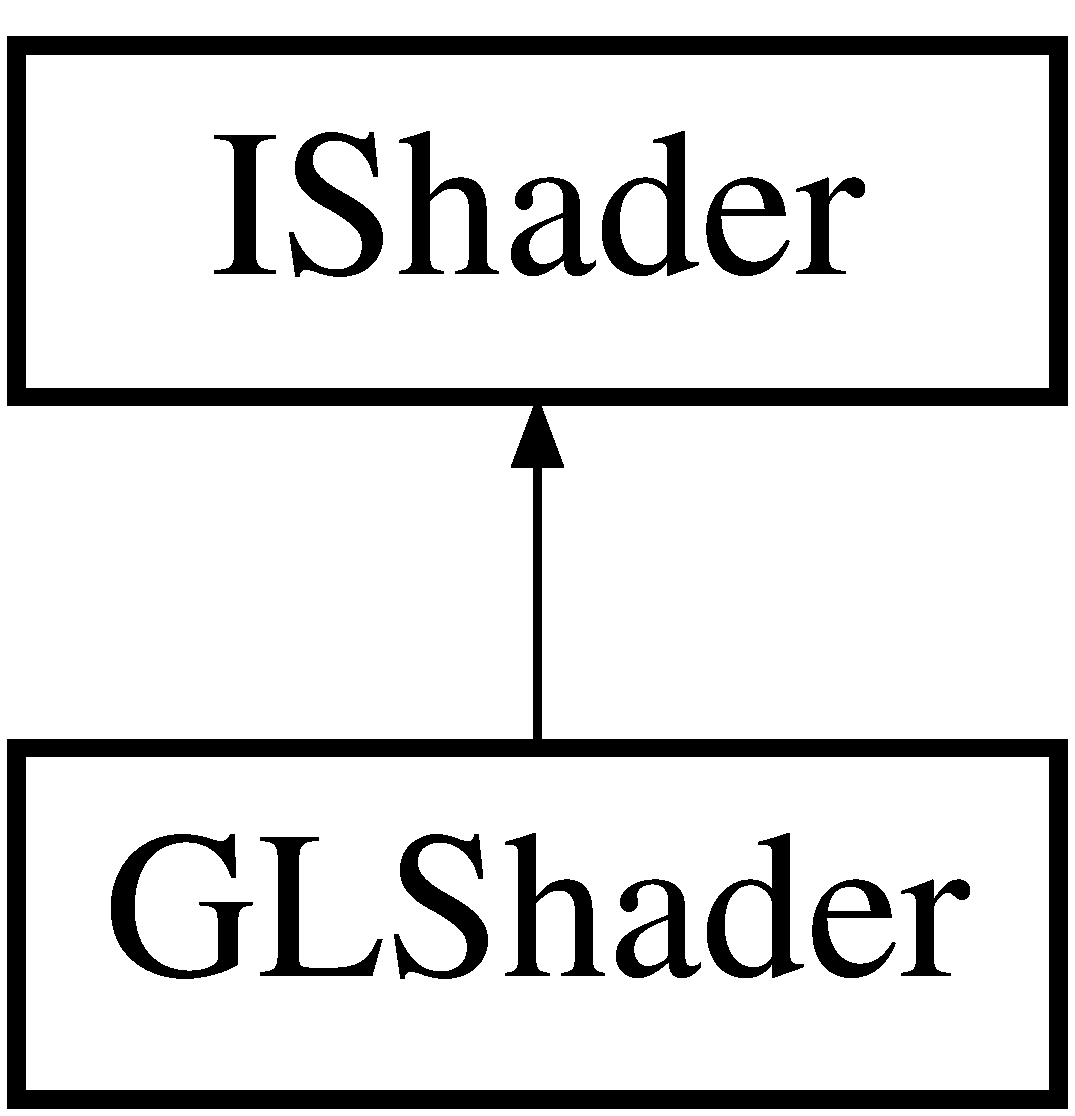
\includegraphics[height=2.000000cm]{class_g_l_shader}
\end{center}
\end{figure}
\subsection*{Public Member Functions}
\begin{DoxyCompactItemize}
\item 
\mbox{\Hypertarget{class_g_l_shader_ad46f3d02c2fa896227aea1e83aa95286}\label{class_g_l_shader_ad46f3d02c2fa896227aea1e83aa95286}} 
{\bfseries G\+L\+Shader} (Shader\+Type shader\+Type, \mbox{\hyperlink{class_not_null}{Not\+Null}}$<$ const char $>$ shader\+Path, \mbox{\hyperlink{class_not_null}{Not\+Null}}$<$ \mbox{\hyperlink{class_g_l_program}{G\+L\+Program}} $>$ gl\+Program) noexcept
\item 
\mbox{\Hypertarget{class_g_l_shader_a6269c8efc2e099fd16275c93c8109b67}\label{class_g_l_shader_a6269c8efc2e099fd16275c93c8109b67}} 
Shader\+Type {\bfseries shader\+Type} () const noexcept override
\item 
\mbox{\Hypertarget{class_g_l_shader_af2012a97450e3b7b1fc5c1569df3a736}\label{class_g_l_shader_af2012a97450e3b7b1fc5c1569df3a736}} 
bool {\bfseries load\+Shader} () noexcept override
\item 
\mbox{\Hypertarget{class_g_l_shader_ab3a52ea131e8d8c322f4398a597f24b9}\label{class_g_l_shader_ab3a52ea131e8d8c322f4398a597f24b9}} 
void {\bfseries activate\+Shader} () const noexcept override
\end{DoxyCompactItemize}
\subsection*{Private Attributes}
\begin{DoxyCompactItemize}
\item 
\mbox{\Hypertarget{class_g_l_shader_ade645efccab5c92733f0238240639544}\label{class_g_l_shader_ade645efccab5c92733f0238240639544}} 
Shader\+Type {\bfseries \+\_\+shader\+Type}
\item 
\mbox{\Hypertarget{class_g_l_shader_a93a52afc055c6497c2029ac7793d611f}\label{class_g_l_shader_a93a52afc055c6497c2029ac7793d611f}} 
const char $\ast$ {\bfseries \+\_\+shader\+Path}
\item 
\mbox{\Hypertarget{class_g_l_shader_a3c8a2c7a3753ede2c60ad537989715d4}\label{class_g_l_shader_a3c8a2c7a3753ede2c60ad537989715d4}} 
\mbox{\hyperlink{class_g_l_program}{G\+L\+Program}} $\ast$ {\bfseries \+\_\+gl\+Program}
\item 
\mbox{\Hypertarget{class_g_l_shader_a98c823944de9e8446adb82701420aa5c}\label{class_g_l_shader_a98c823944de9e8446adb82701420aa5c}} 
G\+Luint {\bfseries \+\_\+shader\+Id}
\end{DoxyCompactItemize}


\subsection{Detailed Description}
Represents an Open\+GL shader. 

The documentation for this class was generated from the following files\+:\begin{DoxyCompactItemize}
\item 
tau/\+Tau\+Engine/include/shader/G\+L\+Shader.\+hpp\item 
tau/\+Tau\+Engine/src/G\+L\+Shader.\+cpp\end{DoxyCompactItemize}

\hypertarget{structstd_1_1hash_3_01_string_01_4}{}\section{std\+:\+:hash$<$ String $>$ Struct Template Reference}
\label{structstd_1_1hash_3_01_string_01_4}\index{std\+::hash$<$ String $>$@{std\+::hash$<$ String $>$}}
\subsection*{Public Member Functions}
\begin{DoxyCompactItemize}
\item 
\mbox{\Hypertarget{structstd_1_1hash_3_01_string_01_4_a05ff12c8d95ebf32c6eaf61c688d0bce}\label{structstd_1_1hash_3_01_string_01_4_a05ff12c8d95ebf32c6eaf61c688d0bce}} 
size\+\_\+t {\bfseries operator()} (const \mbox{\hyperlink{class_string}{String}} \&str) const
\end{DoxyCompactItemize}


The documentation for this struct was generated from the following file\+:\begin{DoxyCompactItemize}
\item 
tau/\+Tau\+Engine/include/String.\+hpp\end{DoxyCompactItemize}

\hypertarget{class_i18n}{}\section{I18n Class Reference}
\label{class_i18n}\index{I18n@{I18n}}
\subsection*{Public Member Functions}
\begin{DoxyCompactItemize}
\item 
\mbox{\Hypertarget{class_i18n_a7567052f24dfcba57fc2a88b67720199}\label{class_i18n_a7567052f24dfcba57fc2a88b67720199}} 
void {\bfseries load\+Translations} (const char $\ast$file)
\end{DoxyCompactItemize}
\subsection*{Private Attributes}
\begin{DoxyCompactItemize}
\item 
\mbox{\Hypertarget{class_i18n_ae8e0a657d30a2f3acecaa0c531719ada}\label{class_i18n_ae8e0a657d30a2f3acecaa0c531719ada}} 
std\+::unordered\+\_\+map$<$ \mbox{\hyperlink{class_string}{String}}, const char $\ast$ $>$ {\bfseries \+\_\+translations}
\end{DoxyCompactItemize}


The documentation for this class was generated from the following file\+:\begin{DoxyCompactItemize}
\item 
tau/\+Tau\+Engine/include/I18n.\+hpp\end{DoxyCompactItemize}

\hypertarget{class_item}{}\section{Item Class Reference}
\label{class_item}\index{Item@{Item}}
\subsection*{Private Attributes}
\begin{DoxyCompactItemize}
\item 
\mbox{\Hypertarget{class_item_a60e04b77db4bdd6b7f7095c1186f8163}\label{class_item_a60e04b77db4bdd6b7f7095c1186f8163}} 
const char $\ast$ {\bfseries \+\_\+unlocalized\+Name}
\item 
\mbox{\Hypertarget{class_item_a48ebca69f9093a000ff5bdfc0a7086be}\label{class_item_a48ebca69f9093a000ff5bdfc0a7086be}} 
const char $\ast$ {\bfseries \+\_\+localized\+Name}
\end{DoxyCompactItemize}


The documentation for this class was generated from the following file\+:\begin{DoxyCompactItemize}
\item 
tau/\+Tau\+Editor/include/Item.\+hpp\end{DoxyCompactItemize}

\hypertarget{class_not_null}{}\section{Not\+Null$<$ \+\_\+T $>$ Class Template Reference}
\label{class_not_null}\index{Not\+Null$<$ \+\_\+\+T $>$@{Not\+Null$<$ \+\_\+\+T $>$}}


{\ttfamily \#include $<$Safeties.\+hpp$>$}

\subsection*{Public Member Functions}
\begin{DoxyCompactItemize}
\item 
\mbox{\Hypertarget{class_not_null_a9dcb748fa5f970539d6af6576ade2753}\label{class_not_null_a9dcb748fa5f970539d6af6576ade2753}} 
{\bfseries Not\+Null} (\+\_\+T $\ast$t) noexcept
\item 
\mbox{\Hypertarget{class_not_null_a4b458914da5d8340a1cfe94cfbcde908}\label{class_not_null_a4b458914da5d8340a1cfe94cfbcde908}} 
{\bfseries Not\+Null} (const \mbox{\hyperlink{class_not_null}{Not\+Null}} \&copy) noexcept
\item 
\mbox{\Hypertarget{class_not_null_a37079630d122047b42e48a9cd7f02656}\label{class_not_null_a37079630d122047b42e48a9cd7f02656}} 
{\bfseries Not\+Null} (\mbox{\hyperlink{class_not_null}{Not\+Null}} \&\&move) noexcept
\item 
\mbox{\Hypertarget{class_not_null_a37305975da9446b42d07b9e9289283a0}\label{class_not_null_a37305975da9446b42d07b9e9289283a0}} 
\mbox{\hyperlink{class_not_null}{Not\+Null}} \& {\bfseries operator=} (const \mbox{\hyperlink{class_not_null}{Not\+Null}} \&copy) noexcept
\item 
\mbox{\Hypertarget{class_not_null_af560eafc386eee76282acb211dbc9ffc}\label{class_not_null_af560eafc386eee76282acb211dbc9ffc}} 
\mbox{\hyperlink{class_not_null}{Not\+Null}} \& {\bfseries operator=} (\mbox{\hyperlink{class_not_null}{Not\+Null}} \&\&move) noexcept
\item 
\mbox{\Hypertarget{class_not_null_afea5aad89957cc45cc0a30debb3fda96}\label{class_not_null_afea5aad89957cc45cc0a30debb3fda96}} 
\+\_\+T \& {\bfseries operator$\ast$} () noexcept
\item 
\mbox{\Hypertarget{class_not_null_a20cbb11e1872d81e4fef9ff3a52b0ba3}\label{class_not_null_a20cbb11e1872d81e4fef9ff3a52b0ba3}} 
\+\_\+T \& {\bfseries operator$\ast$} () const noexcept
\item 
\mbox{\Hypertarget{class_not_null_abd60b54ef1abad202f3650cfdcc53bab}\label{class_not_null_abd60b54ef1abad202f3650cfdcc53bab}} 
\+\_\+T $\ast$ {\bfseries operator-\/$>$} () noexcept
\item 
\mbox{\Hypertarget{class_not_null_a251325b0c267e160e27a1e91a9d78474}\label{class_not_null_a251325b0c267e160e27a1e91a9d78474}} 
\+\_\+T $\ast$ {\bfseries operator-\/$>$} () const noexcept
\item 
\mbox{\Hypertarget{class_not_null_a80b0753670061906773ac549db8d178e}\label{class_not_null_a80b0753670061906773ac549db8d178e}} 
\+\_\+T $\ast$ {\bfseries operator()} () noexcept
\item 
\mbox{\Hypertarget{class_not_null_aa03cff48b0bbdb4e42847bb324ea48dd}\label{class_not_null_aa03cff48b0bbdb4e42847bb324ea48dd}} 
\+\_\+T $\ast$ {\bfseries operator()} () const noexcept
\item 
\mbox{\Hypertarget{class_not_null_a2ede1e0c6322802b2b3db02075700618}\label{class_not_null_a2ede1e0c6322802b2b3db02075700618}} 
{\bfseries operator \+\_\+\+T $\ast$} () noexcept
\item 
\mbox{\Hypertarget{class_not_null_a8f78e7f813813d1ba836b1f050a59a03}\label{class_not_null_a8f78e7f813813d1ba836b1f050a59a03}} 
{\bfseries operator \+\_\+\+T $\ast$} () const noexcept
\end{DoxyCompactItemize}
\subsection*{Public Attributes}
\begin{DoxyCompactItemize}
\item 
\mbox{\Hypertarget{class_not_null_a6fb57bf2755aba617fa008802f084593}\label{class_not_null_a6fb57bf2755aba617fa008802f084593}} 
\+\_\+T $\ast$ {\bfseries \+\_\+t}
\end{DoxyCompactItemize}


\subsection{Detailed Description}
\subsubsection*{template$<$typename \+\_\+T$>$\newline
class Not\+Null$<$ \+\_\+\+T $>$}

A wrapper to print an error and trigger a breakpoint if a value is null. 

The documentation for this class was generated from the following file\+:\begin{DoxyCompactItemize}
\item 
tau/\+Tau\+Utils/include/Safeties.\+hpp\end{DoxyCompactItemize}

\hypertarget{class_string}{}\section{String Class Reference}
\label{class_string}\index{String@{String}}
\subsection*{Public Member Functions}
\begin{DoxyCompactItemize}
\item 
\mbox{\Hypertarget{class_string_a227778609438ca052a4b7f325c1f0502}\label{class_string_a227778609438ca052a4b7f325c1f0502}} 
{\bfseries String} (\mbox{\hyperlink{class_not_null}{Not\+Null}}$<$ const char $>$ string) noexcept
\item 
\mbox{\Hypertarget{class_string_a4b39c4282829506796cf9c1d09538b6c}\label{class_string_a4b39c4282829506796cf9c1d09538b6c}} 
{\bfseries String} (const char $\ast$string) noexcept
\item 
\mbox{\Hypertarget{class_string_a4f8f3179fcb176ac3d204094426a5ada}\label{class_string_a4f8f3179fcb176ac3d204094426a5ada}} 
{\bfseries String} (const \mbox{\hyperlink{class_string}{String}} \&copy) noexcept=default
\item 
\mbox{\Hypertarget{class_string_add2fb3ec45b7fe597bae40ed09ee0785}\label{class_string_add2fb3ec45b7fe597bae40ed09ee0785}} 
{\bfseries String} (\mbox{\hyperlink{class_string}{String}} \&\&move) noexcept
\item 
\mbox{\Hypertarget{class_string_ab509631465fd32f0e1ec84d7087a304f}\label{class_string_ab509631465fd32f0e1ec84d7087a304f}} 
\mbox{\hyperlink{class_string}{String}} \& {\bfseries operator=} (const \mbox{\hyperlink{class_string}{String}} \&copy) noexcept=default
\item 
\mbox{\Hypertarget{class_string_a374418081acd87d867367ae823861ee0}\label{class_string_a374418081acd87d867367ae823861ee0}} 
\mbox{\hyperlink{class_string}{String}} \& {\bfseries operator=} (\mbox{\hyperlink{class_string}{String}} \&\&move) noexcept
\item 
\mbox{\Hypertarget{class_string_a8fe82324a99bae66cab74d308fe22e1d}\label{class_string_a8fe82324a99bae66cab74d308fe22e1d}} 
Non\+Null const char $\ast$ {\bfseries c\+\_\+str} () const noexcept
\item 
\mbox{\Hypertarget{class_string_a5f96a6ada25cdf853b7a1f39783ce64d}\label{class_string_a5f96a6ada25cdf853b7a1f39783ce64d}} 
u32 {\bfseries length} () const noexcept
\item 
\mbox{\Hypertarget{class_string_a6ce9d8ee2ecadf146944dc48b1fb292f}\label{class_string_a6ce9d8ee2ecadf146944dc48b1fb292f}} 
{\bfseries operator const char $\ast$} () const noexcept
\item 
\mbox{\Hypertarget{class_string_aeb704926e1c7309c55c281b2e8078830}\label{class_string_aeb704926e1c7309c55c281b2e8078830}} 
u32 {\bfseries operator()} () const noexcept
\item 
\mbox{\Hypertarget{class_string_a8fd0c05e3a9ee76784cde5818b9146c7}\label{class_string_a8fd0c05e3a9ee76784cde5818b9146c7}} 
u32 {\bfseries hash\+Code} () const noexcept
\item 
\mbox{\Hypertarget{class_string_a8a6813758d1896dbf09665775416800a}\label{class_string_a8a6813758d1896dbf09665775416800a}} 
bool {\bfseries equals} (const \mbox{\hyperlink{class_string}{String}} \&other) const noexcept
\item 
\mbox{\Hypertarget{class_string_a4f5c978f41165bed85197a8c15e2c39e}\label{class_string_a4f5c978f41165bed85197a8c15e2c39e}} 
i32 {\bfseries compare\+To} (const \mbox{\hyperlink{class_string}{String}} \&other) const noexcept
\item 
\mbox{\Hypertarget{class_string_a039a56a34f761f9fd60f0c292e739de7}\label{class_string_a039a56a34f761f9fd60f0c292e739de7}} 
bool {\bfseries operator==} (const \mbox{\hyperlink{class_string}{String}} \&other) const noexcept
\item 
\mbox{\Hypertarget{class_string_a7952b22541d9ea1550b03da964274fca}\label{class_string_a7952b22541d9ea1550b03da964274fca}} 
bool {\bfseries operator!=} (const \mbox{\hyperlink{class_string}{String}} \&other) const noexcept
\item 
\mbox{\Hypertarget{class_string_ad97ae77967881f018f12c1d73e10655a}\label{class_string_ad97ae77967881f018f12c1d73e10655a}} 
bool {\bfseries operator$<$} (const \mbox{\hyperlink{class_string}{String}} \&other) const noexcept
\item 
\mbox{\Hypertarget{class_string_a4e553df61d67f5a74b11baab4846743f}\label{class_string_a4e553df61d67f5a74b11baab4846743f}} 
bool {\bfseries operator$>$} (const \mbox{\hyperlink{class_string}{String}} \&other) const noexcept
\item 
\mbox{\Hypertarget{class_string_adb110f5512e42a8cb4562a78a41591b9}\label{class_string_adb110f5512e42a8cb4562a78a41591b9}} 
bool {\bfseries operator$<$=} (const \mbox{\hyperlink{class_string}{String}} \&other) const noexcept
\item 
\mbox{\Hypertarget{class_string_ab3dd8e113a19317a31d9ca91c78b6ec0}\label{class_string_ab3dd8e113a19317a31d9ca91c78b6ec0}} 
bool {\bfseries operator$>$=} (const \mbox{\hyperlink{class_string}{String}} \&other) const noexcept
\end{DoxyCompactItemize}
\subsection*{Static Private Member Functions}
\begin{DoxyCompactItemize}
\item 
\mbox{\Hypertarget{class_string_ada0c2bbb5447b10a4a4bf52f777bcbda}\label{class_string_ada0c2bbb5447b10a4a4bf52f777bcbda}} 
static u32 {\bfseries find\+Hash\+Code} (Non\+Null const char $\ast$str) noexcept
\end{DoxyCompactItemize}
\subsection*{Private Attributes}
\begin{DoxyCompactItemize}
\item 
\mbox{\Hypertarget{class_string_a5daeeb0eb9fb5a569e296f59f1e0c6c6}\label{class_string_a5daeeb0eb9fb5a569e296f59f1e0c6c6}} 
const char $\ast$ {\bfseries \+\_\+string}
\item 
\mbox{\Hypertarget{class_string_afbd91c4ee8068ee71deb5672bdf98204}\label{class_string_afbd91c4ee8068ee71deb5672bdf98204}} 
u32 {\bfseries \+\_\+length}
\item 
\mbox{\Hypertarget{class_string_a2cb285b307912ad2ac5cfe700cd11827}\label{class_string_a2cb285b307912ad2ac5cfe700cd11827}} 
u32 {\bfseries \+\_\+hash}
\end{DoxyCompactItemize}


The documentation for this class was generated from the following files\+:\begin{DoxyCompactItemize}
\item 
tau/\+Tau\+Engine/include/String.\+hpp\item 
tau/\+Tau\+Engine/src/String.\+cpp\end{DoxyCompactItemize}

\hypertarget{class_t_u_i_d}{}\section{T\+U\+ID Class Reference}
\label{class_t_u_i_d}\index{T\+U\+ID@{T\+U\+ID}}


{\ttfamily \#include $<$T\+U\+I\+D.\+hpp$>$}

\subsection*{Public Member Functions}
\begin{DoxyCompactItemize}
\item 
\mbox{\Hypertarget{class_t_u_i_d_a9b95de9b3f8a66238154066825245d48}\label{class_t_u_i_d_a9b95de9b3f8a66238154066825245d48}} 
{\bfseries T\+U\+ID} (u64 high\+Bits, u64 low\+Bits) noexcept
\item 
\mbox{\Hypertarget{class_t_u_i_d_a56805ea07350451e3b4895dbed7350b0}\label{class_t_u_i_d_a56805ea07350451e3b4895dbed7350b0}} 
u64 {\bfseries high\+Bits} () const noexcept
\item 
\mbox{\Hypertarget{class_t_u_i_d_ae90c5736b12ead378662d3771247e2e6}\label{class_t_u_i_d_ae90c5736b12ead378662d3771247e2e6}} 
u64 {\bfseries low\+Bits} () const noexcept
\item 
\mbox{\Hypertarget{class_t_u_i_d_a41a41b4dba721ac1b61277c12b3c86ac}\label{class_t_u_i_d_a41a41b4dba721ac1b61277c12b3c86ac}} 
void {\bfseries to\+String} (char str\mbox{[}38\mbox{]}) const noexcept
\end{DoxyCompactItemize}
\subsection*{Static Public Member Functions}
\begin{DoxyCompactItemize}
\item 
\mbox{\Hypertarget{class_t_u_i_d_ae4de4649155bc36054f9c1f0fe40eabb}\label{class_t_u_i_d_ae4de4649155bc36054f9c1f0fe40eabb}} 
static \mbox{\hyperlink{class_t_u_i_d}{T\+U\+ID}} {\bfseries generate} () noexcept
\end{DoxyCompactItemize}
\subsection*{Private Attributes}
\begin{DoxyCompactItemize}
\item 
\mbox{\Hypertarget{class_t_u_i_d_a2fb2939d72f8dbf73fb421529b13dd80}\label{class_t_u_i_d_a2fb2939d72f8dbf73fb421529b13dd80}} 
u64 {\bfseries \+\_\+high\+Bits}
\item 
\mbox{\Hypertarget{class_t_u_i_d_a6767938b10a94b4a69fdbb4b8b7f3875}\label{class_t_u_i_d_a6767938b10a94b4a69fdbb4b8b7f3875}} 
u64 {\bfseries \+\_\+low\+Bits}
\end{DoxyCompactItemize}


\subsection{Detailed Description}
Tau Unique I\+Dentification.

A knockoff U\+U\+ID \char`\"{}guaranteed\char`\"{} to be unique within the engine. 

The documentation for this class was generated from the following files\+:\begin{DoxyCompactItemize}
\item 
tau/\+Tau\+Engine/include/\mbox{\hyperlink{_t_u_i_d_8hpp}{T\+U\+I\+D.\+hpp}}\item 
tau/\+Tau\+Engine/src/T\+U\+I\+D.\+cpp\end{DoxyCompactItemize}

\hypertarget{struct_type_name}{}\section{Type\+Name$<$ \+\_\+T $>$ Struct Template Reference}
\label{struct_type_name}\index{Type\+Name$<$ \+\_\+\+T $>$@{Type\+Name$<$ \+\_\+\+T $>$}}
\subsection*{Static Public Member Functions}
\begin{DoxyCompactItemize}
\item 
\mbox{\Hypertarget{struct_type_name_ab7d1e1a476a249512f1809d907ca93b3}\label{struct_type_name_ab7d1e1a476a249512f1809d907ca93b3}} 
static const char $\ast$ {\bfseries Name} ()
\end{DoxyCompactItemize}


The documentation for this struct was generated from the following file\+:\begin{DoxyCompactItemize}
\item 
Tau\+Utils/include/Template.\+hpp\end{DoxyCompactItemize}

\hypertarget{class_vector3f}{}\section{Vector3f Class Reference}
\label{class_vector3f}\index{Vector3f@{Vector3f}}
\subsection*{Public Member Functions}
\begin{DoxyCompactItemize}
\item 
\mbox{\Hypertarget{class_vector3f_a4e8abfa18d76f6c3191a4db038f9ec31}\label{class_vector3f_a4e8abfa18d76f6c3191a4db038f9ec31}} 
{\bfseries Vector3f} (const \+\_\+\+\_\+m128 vec) noexcept
\item 
\mbox{\Hypertarget{class_vector3f_ac4ea096310c4950d9857c70c2924507d}\label{class_vector3f_ac4ea096310c4950d9857c70c2924507d}} 
{\bfseries Vector3f} (const \+\_\+\+\_\+m128i vec) noexcept
\item 
\mbox{\Hypertarget{class_vector3f_af43fca5b619035fa41be55aed8c58661}\label{class_vector3f_af43fca5b619035fa41be55aed8c58661}} 
{\bfseries Vector3f} (const float x, const float y, const float z) noexcept
\item 
\mbox{\Hypertarget{class_vector3f_ae959ab0a36b30b77761ba9d014942509}\label{class_vector3f_ae959ab0a36b30b77761ba9d014942509}} 
{\bfseries Vector3f} (const i32 x, const i32 y, const i32 z) noexcept
\item 
\mbox{\Hypertarget{class_vector3f_a5a6b53892d0a23acf77a8f0cff92b558}\label{class_vector3f_a5a6b53892d0a23acf77a8f0cff92b558}} 
{\bfseries Vector3f} (const float filler) noexcept
\item 
\mbox{\Hypertarget{class_vector3f_a2b00c2d99d90c9d6284c95c4f2c50d51}\label{class_vector3f_a2b00c2d99d90c9d6284c95c4f2c50d51}} 
{\bfseries Vector3f} (const i32 filler) noexcept
\item 
\mbox{\Hypertarget{class_vector3f_abfed8c262b9cecefb387a5cf9fd8f288}\label{class_vector3f_abfed8c262b9cecefb387a5cf9fd8f288}} 
{\bfseries Vector3f} (const Comp\+Vec4 \&data) noexcept
\item 
\mbox{\Hypertarget{class_vector3f_ab727e3f9844af287191e09618abd43ab}\label{class_vector3f_ab727e3f9844af287191e09618abd43ab}} 
\mbox{\hyperlink{class_vector3f}{Vector3f}} \& {\bfseries operator=} (const float filler) noexcept
\item 
\mbox{\Hypertarget{class_vector3f_a89526604dd962785343702f6e2cde315}\label{class_vector3f_a89526604dd962785343702f6e2cde315}} 
\mbox{\hyperlink{class_vector3f}{Vector3f}} \& {\bfseries operator=} (const i32 filler) noexcept
\item 
\mbox{\Hypertarget{class_vector3f_a1006fa2a3639ae7e8649ebb860018b69}\label{class_vector3f_a1006fa2a3639ae7e8649ebb860018b69}} 
\mbox{\hyperlink{class_vector3f}{Vector3f}} \& {\bfseries operator=} (const Comp\+Vec4 \&copy) noexcept
\item 
\mbox{\Hypertarget{class_vector3f_a566ac4e4e5715603b3e223493e0ea69c}\label{class_vector3f_a566ac4e4e5715603b3e223493e0ea69c}} 
float {\bfseries x} () const noexcept
\item 
\mbox{\Hypertarget{class_vector3f_a22720415e42546a611b930a7df983086}\label{class_vector3f_a22720415e42546a611b930a7df983086}} 
float {\bfseries y} () const noexcept
\item 
\mbox{\Hypertarget{class_vector3f_a48cc596b0a649c142009c76f7cd4744c}\label{class_vector3f_a48cc596b0a649c142009c76f7cd4744c}} 
float {\bfseries z} () const noexcept
\item 
\mbox{\Hypertarget{class_vector3f_afa3ffe0ecd24ffd3390751fc4f1484c9}\label{class_vector3f_afa3ffe0ecd24ffd3390751fc4f1484c9}} 
float \& {\bfseries x} () noexcept
\item 
\mbox{\Hypertarget{class_vector3f_a5a06e1be3e79f5e7b9042dcfe46c667c}\label{class_vector3f_a5a06e1be3e79f5e7b9042dcfe46c667c}} 
float \& {\bfseries y} () noexcept
\item 
\mbox{\Hypertarget{class_vector3f_a16212f4681911cc81a3f6209807ca3ad}\label{class_vector3f_a16212f4681911cc81a3f6209807ca3ad}} 
float \& {\bfseries z} () noexcept
\item 
\mbox{\Hypertarget{class_vector3f_ab4c695a15779fb8963ecf49b53c994ab}\label{class_vector3f_ab4c695a15779fb8963ecf49b53c994ab}} 
Comp\+Vec4 {\bfseries data} () const noexcept
\item 
\mbox{\Hypertarget{class_vector3f_a4f9ddb65d252b26ede9acec335f338f6}\label{class_vector3f_a4f9ddb65d252b26ede9acec335f338f6}} 
Comp\+Vec4 \& {\bfseries data} () noexcept
\item 
\mbox{\Hypertarget{class_vector3f_ac278f1d3dca951774ca77dbd9350367f}\label{class_vector3f_ac278f1d3dca951774ca77dbd9350367f}} 
{\bfseries operator Comp\+Vec4} () const noexcept
\item 
\mbox{\Hypertarget{class_vector3f_a32a93d66903416a2e7f6e18b900ef986}\label{class_vector3f_a32a93d66903416a2e7f6e18b900ef986}} 
{\bfseries operator Comp\+Vec4 \&} () noexcept
\item 
\mbox{\Hypertarget{class_vector3f_abebb5adb6603e8d0bc54c426bd034eab}\label{class_vector3f_abebb5adb6603e8d0bc54c426bd034eab}} 
{\bfseries R\+A\+W\+\_\+\+V\+E\+C\+\_\+\+F\+U\+NC} (\mbox{\hyperlink{class_vector3f}{Vector3f}} \&, add, noexcept)
\item 
\mbox{\Hypertarget{class_vector3f_a0ed84add7cd4af54e1e60d4fa18e38a6}\label{class_vector3f_a0ed84add7cd4af54e1e60d4fa18e38a6}} 
{\bfseries R\+A\+W\+\_\+\+V\+E\+C\+\_\+\+F\+U\+NC} (\mbox{\hyperlink{class_vector3f}{Vector3f}} \&, sub, noexcept)
\item 
\mbox{\Hypertarget{class_vector3f_adb73681adf2f1dafdfe38952520426a8}\label{class_vector3f_adb73681adf2f1dafdfe38952520426a8}} 
{\bfseries R\+A\+W\+\_\+\+V\+E\+C\+\_\+\+F\+U\+NC} (\mbox{\hyperlink{class_vector3f}{Vector3f}}, addC, const noexcept)
\item 
\mbox{\Hypertarget{class_vector3f_ad4b799dada66a42da73fcc69ac80dbae}\label{class_vector3f_ad4b799dada66a42da73fcc69ac80dbae}} 
{\bfseries R\+A\+W\+\_\+\+V\+E\+C\+\_\+\+F\+U\+NC} (\mbox{\hyperlink{class_vector3f}{Vector3f}}, subC, const noexcept)
\item 
\mbox{\Hypertarget{class_vector3f_adbb945616bc1fe866c7a91f5b959a6b7}\label{class_vector3f_adbb945616bc1fe866c7a91f5b959a6b7}} 
\mbox{\hyperlink{class_vector3f}{Vector3f}} \& {\bfseries add} (const Comp\+Vec4 \&data) noexcept
\item 
\mbox{\Hypertarget{class_vector3f_ac46dbd570369dc7b92f058745797bb7e}\label{class_vector3f_ac46dbd570369dc7b92f058745797bb7e}} 
\mbox{\hyperlink{class_vector3f}{Vector3f}} \& {\bfseries sub} (const Comp\+Vec4 \&data) noexcept
\item 
\mbox{\Hypertarget{class_vector3f_af0e7dc08eab2ec9a2302d4121102defb}\label{class_vector3f_af0e7dc08eab2ec9a2302d4121102defb}} 
\mbox{\hyperlink{class_vector3f}{Vector3f}} {\bfseries addC} (const Comp\+Vec4 \&data) const noexcept
\item 
\mbox{\Hypertarget{class_vector3f_a53cca8b48539285982e87e0f9d6901b5}\label{class_vector3f_a53cca8b48539285982e87e0f9d6901b5}} 
\mbox{\hyperlink{class_vector3f}{Vector3f}} {\bfseries subC} (const Comp\+Vec4 \&data) const noexcept
\item 
\mbox{\Hypertarget{class_vector3f_a48c64756150fc5e4219be4c2d9d3fec0}\label{class_vector3f_a48c64756150fc5e4219be4c2d9d3fec0}} 
{\bfseries S\+C\+A\+L\+A\+R\+\_\+\+M\+A\+TH} (add)
\item 
\mbox{\Hypertarget{class_vector3f_ad28edcbe986adb1f0b2762451cbeed88}\label{class_vector3f_ad28edcbe986adb1f0b2762451cbeed88}} 
{\bfseries S\+C\+A\+L\+A\+R\+\_\+\+M\+A\+TH} (sub)
\item 
\mbox{\Hypertarget{class_vector3f_a511bb22386ab52853b2946765829db30}\label{class_vector3f_a511bb22386ab52853b2946765829db30}} 
{\bfseries S\+C\+A\+L\+A\+R\+\_\+\+M\+A\+TH} (mul)
\item 
\mbox{\Hypertarget{class_vector3f_a0ada95ece11bb564008c953b5be2a184}\label{class_vector3f_a0ada95ece11bb564008c953b5be2a184}} 
{\bfseries S\+C\+A\+L\+A\+R\+\_\+\+M\+A\+TH} (div)
\item 
\mbox{\Hypertarget{class_vector3f_a980ace62ba0cd3fb1c9ce3da2f66ffa6}\label{class_vector3f_a980ace62ba0cd3fb1c9ce3da2f66ffa6}} 
\mbox{\hyperlink{class_vector3f}{Vector3f}} \& {\bfseries scale} (const float scalar) noexcept
\item 
\mbox{\Hypertarget{class_vector3f_a38d4146c614cf58391833357049b12ab}\label{class_vector3f_a38d4146c614cf58391833357049b12ab}} 
\mbox{\hyperlink{class_vector3f}{Vector3f}} \& {\bfseries scale} (const i32 scalar) noexcept
\item 
\mbox{\Hypertarget{class_vector3f_a332ae913d390617d745358e9adc3207a}\label{class_vector3f_a332ae913d390617d745358e9adc3207a}} 
\mbox{\hyperlink{class_vector3f}{Vector3f}} {\bfseries scaleC} (const float scalar) const noexcept
\item 
\mbox{\Hypertarget{class_vector3f_a27b81e2719d74e97a1e76d5f8cf2d72f}\label{class_vector3f_a27b81e2719d74e97a1e76d5f8cf2d72f}} 
\mbox{\hyperlink{class_vector3f}{Vector3f}} {\bfseries scaleC} (const i32 scalar) const noexcept
\item 
\mbox{\Hypertarget{class_vector3f_a8e74365d4f74663c7a6457feb9c53387}\label{class_vector3f_a8e74365d4f74663c7a6457feb9c53387}} 
\mbox{\hyperlink{class_vector3f}{Vector3f}} \& {\bfseries negate} () noexcept
\item 
\mbox{\Hypertarget{class_vector3f_a31dd164efbe43832619fcf8415272bd5}\label{class_vector3f_a31dd164efbe43832619fcf8415272bd5}} 
\mbox{\hyperlink{class_vector3f}{Vector3f}} {\bfseries negate\+Copy} () const noexcept
\item 
\mbox{\Hypertarget{class_vector3f_a8644088d07ec066c795fc565dcdb29e8}\label{class_vector3f_a8644088d07ec066c795fc565dcdb29e8}} 
\mbox{\hyperlink{class_vector3f}{Vector3f}} \& {\bfseries neg} () noexcept
\item 
\mbox{\Hypertarget{class_vector3f_a4132ae254a350ee1165b71c01742c728}\label{class_vector3f_a4132ae254a350ee1165b71c01742c728}} 
\mbox{\hyperlink{class_vector3f}{Vector3f}} {\bfseries neg\+Copy} () const noexcept
\item 
\mbox{\Hypertarget{class_vector3f_a035fae5d2e8e73a5e8ca16a91d4ebd24}\label{class_vector3f_a035fae5d2e8e73a5e8ca16a91d4ebd24}} 
float {\bfseries magnitude\+Squared} () const noexcept
\item 
\mbox{\Hypertarget{class_vector3f_a9921b92d7fd31fc28bab947d061d1533}\label{class_vector3f_a9921b92d7fd31fc28bab947d061d1533}} 
float {\bfseries magnitude} () const noexcept
\item 
\mbox{\Hypertarget{class_vector3f_a774748eb74ea927b36b214737467264e}\label{class_vector3f_a774748eb74ea927b36b214737467264e}} 
float {\bfseries length\+Squared} () const noexcept
\item 
\mbox{\Hypertarget{class_vector3f_ab5ceb51ef9e48bb3776ed179e9f729b6}\label{class_vector3f_ab5ceb51ef9e48bb3776ed179e9f729b6}} 
float {\bfseries length} () const noexcept
\item 
\mbox{\Hypertarget{class_vector3f_a4fa576a7824df90857e83304587afddd}\label{class_vector3f_a4fa576a7824df90857e83304587afddd}} 
\mbox{\hyperlink{class_vector3f}{Vector3f}} {\bfseries inverse\+Sqrt} () const noexcept
\item 
\mbox{\Hypertarget{class_vector3f_a9b0acc9cad15a49af56c3fc5c3d09965}\label{class_vector3f_a9b0acc9cad15a49af56c3fc5c3d09965}} 
{\bfseries R\+A\+W\+\_\+\+V\+E\+C\+\_\+\+F\+U\+NC} (float, dot, const noexcept)
\item 
\mbox{\Hypertarget{class_vector3f_a292e6718be5165a86cb0f05790f4ab06}\label{class_vector3f_a292e6718be5165a86cb0f05790f4ab06}} 
{\bfseries R\+A\+W\+\_\+\+V\+E\+C\+\_\+\+F\+U\+NC} (\mbox{\hyperlink{class_vector3f}{Vector3f}} \&, cross, noexcept)
\item 
\mbox{\Hypertarget{class_vector3f_a2bcae3d4c31bebe30fe808611ed469f2}\label{class_vector3f_a2bcae3d4c31bebe30fe808611ed469f2}} 
{\bfseries R\+A\+W\+\_\+\+V\+E\+C\+\_\+\+F\+U\+NC} (\mbox{\hyperlink{class_vector3f}{Vector3f}}, crossC, const noexcept)
\item 
\mbox{\Hypertarget{class_vector3f_af722aedce600ad149642c1c822104f28}\label{class_vector3f_af722aedce600ad149642c1c822104f28}} 
float {\bfseries dot} (const Comp\+Vec4 \&data) const noexcept
\item 
\mbox{\Hypertarget{class_vector3f_a21c67c09d5a27cc588d464a2fdb2c1a8}\label{class_vector3f_a21c67c09d5a27cc588d464a2fdb2c1a8}} 
\mbox{\hyperlink{class_vector3f}{Vector3f}} \& {\bfseries cross} (const Comp\+Vec4 \&data) noexcept
\item 
\mbox{\Hypertarget{class_vector3f_aaa1c2e4c5c67b67e31ec30830811dcda}\label{class_vector3f_aaa1c2e4c5c67b67e31ec30830811dcda}} 
\mbox{\hyperlink{class_vector3f}{Vector3f}} {\bfseries crossC} (const Comp\+Vec4 \&data) const noexcept
\item 
\mbox{\Hypertarget{class_vector3f_a9e4da46a9d72284e1bb75cdd07f64c97}\label{class_vector3f_a9e4da46a9d72284e1bb75cdd07f64c97}} 
\mbox{\hyperlink{class_vector3f}{Vector3f}} \& {\bfseries normalize} () noexcept
\item 
\mbox{\Hypertarget{class_vector3f_a4caf414ea37f685de9f080bcbd791203}\label{class_vector3f_a4caf414ea37f685de9f080bcbd791203}} 
\mbox{\hyperlink{class_vector3f}{Vector3f}} {\bfseries normalizeC} () const noexcept
\item 
\mbox{\Hypertarget{class_vector3f_aafd59ed86521aa17c500d2b5ac3838d3}\label{class_vector3f_aafd59ed86521aa17c500d2b5ac3838d3}} 
{\bfseries O\+P\+E\+R\+A\+T\+OR} (\mbox{\hyperlink{class_vector3f}{Vector3f}},+, Comp\+Vec4 \&, const noexcept, addC)
\item 
\mbox{\Hypertarget{class_vector3f_ad3883c24f80f122c7fa1f013170d0bbe}\label{class_vector3f_ad3883c24f80f122c7fa1f013170d0bbe}} 
{\bfseries O\+P\+E\+R\+A\+T\+OR} (\mbox{\hyperlink{class_vector3f}{Vector3f}}, -\/, Comp\+Vec4 \&, const noexcept, subC)
\item 
\mbox{\Hypertarget{class_vector3f_a8360918e7b9e647000d9f9a03918b3e6}\label{class_vector3f_a8360918e7b9e647000d9f9a03918b3e6}} 
{\bfseries O\+P\+E\+R\+A\+T\+OR} (\mbox{\hyperlink{class_vector3f}{Vector3f}}, $\ast$, Comp\+Vec4 \&, const noexcept, crossC)
\item 
\mbox{\Hypertarget{class_vector3f_a1021701786c76b3b11bf563db1be3cdb}\label{class_vector3f_a1021701786c76b3b11bf563db1be3cdb}} 
{\bfseries O\+P\+E\+R\+A\+T\+OR} (\mbox{\hyperlink{class_vector3f}{Vector3f}} \&,+=, Comp\+Vec4 \&, noexcept, add)
\item 
\mbox{\Hypertarget{class_vector3f_acf226a1ec20e129f3721bd3230412745}\label{class_vector3f_acf226a1ec20e129f3721bd3230412745}} 
{\bfseries O\+P\+E\+R\+A\+T\+OR} (\mbox{\hyperlink{class_vector3f}{Vector3f}} \&, -\/=, Comp\+Vec4 \&, noexcept, sub)
\item 
\mbox{\Hypertarget{class_vector3f_a76103dbe4e8e5ce5ea4f67d2fa57eb6b}\label{class_vector3f_a76103dbe4e8e5ce5ea4f67d2fa57eb6b}} 
{\bfseries O\+P\+E\+R\+A\+T\+OR} (\mbox{\hyperlink{class_vector3f}{Vector3f}} \&, $\ast$=, Comp\+Vec4 \&, noexcept, cross)
\item 
\mbox{\Hypertarget{class_vector3f_aa5cdf02ffc57ee17c80ba05f86597a90}\label{class_vector3f_aa5cdf02ffc57ee17c80ba05f86597a90}} 
{\bfseries S\+C\+A\+L\+A\+R\+\_\+\+O\+P\+E\+R\+A\+T\+OR} (\mbox{\hyperlink{class_vector3f}{Vector3f}},+, const noexcept, addC)
\item 
\mbox{\Hypertarget{class_vector3f_a3912940c33698b03767a4509d187b76e}\label{class_vector3f_a3912940c33698b03767a4509d187b76e}} 
{\bfseries S\+C\+A\+L\+A\+R\+\_\+\+O\+P\+E\+R\+A\+T\+OR} (\mbox{\hyperlink{class_vector3f}{Vector3f}}, -\/, const noexcept, subC)
\item 
\mbox{\Hypertarget{class_vector3f_a0e370ab49624383e04d20dad9f8294ea}\label{class_vector3f_a0e370ab49624383e04d20dad9f8294ea}} 
{\bfseries S\+C\+A\+L\+A\+R\+\_\+\+O\+P\+E\+R\+A\+T\+OR} (\mbox{\hyperlink{class_vector3f}{Vector3f}}, $\ast$, const noexcept, mulC)
\item 
\mbox{\Hypertarget{class_vector3f_acde0572b360ea640cff039cb3d829260}\label{class_vector3f_acde0572b360ea640cff039cb3d829260}} 
{\bfseries S\+C\+A\+L\+A\+R\+\_\+\+O\+P\+E\+R\+A\+T\+OR} (\mbox{\hyperlink{class_vector3f}{Vector3f}},/, const noexcept, divC)
\item 
\mbox{\Hypertarget{class_vector3f_a3ed47a71d98e926d317640a22691e66b}\label{class_vector3f_a3ed47a71d98e926d317640a22691e66b}} 
{\bfseries S\+C\+A\+L\+A\+R\+\_\+\+O\+P\+E\+R\+A\+T\+OR} (\mbox{\hyperlink{class_vector3f}{Vector3f}} \&,+=, noexcept, add)
\item 
\mbox{\Hypertarget{class_vector3f_a855c7498a8ebc45706febde31a7af47a}\label{class_vector3f_a855c7498a8ebc45706febde31a7af47a}} 
{\bfseries S\+C\+A\+L\+A\+R\+\_\+\+O\+P\+E\+R\+A\+T\+OR} (\mbox{\hyperlink{class_vector3f}{Vector3f}} \&, -\/=, noexcept, sub)
\item 
\mbox{\Hypertarget{class_vector3f_a6f5460b9e7f65cd514648395538676cc}\label{class_vector3f_a6f5460b9e7f65cd514648395538676cc}} 
{\bfseries S\+C\+A\+L\+A\+R\+\_\+\+O\+P\+E\+R\+A\+T\+OR} (\mbox{\hyperlink{class_vector3f}{Vector3f}} \&, $\ast$=, noexcept, mul)
\item 
\mbox{\Hypertarget{class_vector3f_ab14cd359d52fe6c38d85840808940656}\label{class_vector3f_ab14cd359d52fe6c38d85840808940656}} 
{\bfseries S\+C\+A\+L\+A\+R\+\_\+\+O\+P\+E\+R\+A\+T\+OR} (\mbox{\hyperlink{class_vector3f}{Vector3f}} \&,/=, noexcept, div)
\item 
\mbox{\Hypertarget{class_vector3f_a24c62b1fe1d2f18f9289f36e0b06857c}\label{class_vector3f_a24c62b1fe1d2f18f9289f36e0b06857c}} 
\mbox{\hyperlink{class_vector3f}{Vector3f}} \& {\bfseries operator-\/} () noexcept
\item 
\mbox{\Hypertarget{class_vector3f_a0ae27c6a481043c1e8c1935ccde73b1c}\label{class_vector3f_a0ae27c6a481043c1e8c1935ccde73b1c}} 
\mbox{\hyperlink{class_vector3f}{Vector3f}} {\bfseries operator-\/} () const noexcept
\end{DoxyCompactItemize}
\subsection*{Private Attributes}
\begin{DoxyCompactItemize}
\item 
\mbox{\Hypertarget{class_vector3f_a8dd741fdb0ea0a3bd9aaf0e110b7c45c}\label{class_vector3f_a8dd741fdb0ea0a3bd9aaf0e110b7c45c}} 
Comp\+Vec4 {\bfseries \+\_\+data}
\end{DoxyCompactItemize}


The documentation for this class was generated from the following files\+:\begin{DoxyCompactItemize}
\item 
tau/\+Tau\+Engine/include/maths/Vector3f.\+hpp\item 
tau/\+Tau\+Engine/src/Vector3f.\+cpp\end{DoxyCompactItemize}

\hypertarget{class_vector3i}{}\section{Vector3i Class Reference}
\label{class_vector3i}\index{Vector3i@{Vector3i}}
\subsection*{Public Member Functions}
\begin{DoxyCompactItemize}
\item 
\mbox{\Hypertarget{class_vector3i_a6f71559a7dbbb35f86600067eecfc5f3}\label{class_vector3i_a6f71559a7dbbb35f86600067eecfc5f3}} 
{\bfseries Vector3i} (const \+\_\+\+\_\+m128 vec) noexcept
\item 
\mbox{\Hypertarget{class_vector3i_a36784de68b048cdd7fb77b5d805f3d20}\label{class_vector3i_a36784de68b048cdd7fb77b5d805f3d20}} 
{\bfseries Vector3i} (const \+\_\+\+\_\+m128i vec) noexcept
\item 
\mbox{\Hypertarget{class_vector3i_a8bec55b58926bdeab4ffb2e531bc81f6}\label{class_vector3i_a8bec55b58926bdeab4ffb2e531bc81f6}} 
{\bfseries Vector3i} (const float x, const float y, const float z) noexcept
\item 
\mbox{\Hypertarget{class_vector3i_a8636644f367b9abdaf51ef62d46c1afc}\label{class_vector3i_a8636644f367b9abdaf51ef62d46c1afc}} 
{\bfseries Vector3i} (const i32 x, const i32 y, const i32 z) noexcept
\item 
\mbox{\Hypertarget{class_vector3i_a12b6865ddaecb29b6614ac46d66b6596}\label{class_vector3i_a12b6865ddaecb29b6614ac46d66b6596}} 
{\bfseries Vector3i} (const float filler) noexcept
\item 
\mbox{\Hypertarget{class_vector3i_aaa914a33dc10a8e43baa7a9abf85d019}\label{class_vector3i_aaa914a33dc10a8e43baa7a9abf85d019}} 
{\bfseries Vector3i} (const i32 filler) noexcept
\item 
\mbox{\Hypertarget{class_vector3i_a7bc7804edc326bddd6809633bf8a38a7}\label{class_vector3i_a7bc7804edc326bddd6809633bf8a38a7}} 
{\bfseries Vector3i} (const Comp\+Vec4 \&data) noexcept
\item 
\mbox{\Hypertarget{class_vector3i_ada108ce6d6df13efa03a5a34b52cd0c0}\label{class_vector3i_ada108ce6d6df13efa03a5a34b52cd0c0}} 
\mbox{\hyperlink{class_vector3i}{Vector3i}} \& {\bfseries operator=} (const float filler) noexcept
\item 
\mbox{\Hypertarget{class_vector3i_a8d96475c2c165d7bee9707f9e5ff8dff}\label{class_vector3i_a8d96475c2c165d7bee9707f9e5ff8dff}} 
\mbox{\hyperlink{class_vector3i}{Vector3i}} \& {\bfseries operator=} (const i32 filler) noexcept
\item 
\mbox{\Hypertarget{class_vector3i_a11e3ae350fd9cde98aaa4211270e256a}\label{class_vector3i_a11e3ae350fd9cde98aaa4211270e256a}} 
\mbox{\hyperlink{class_vector3i}{Vector3i}} \& {\bfseries operator=} (const Comp\+Vec4 \&copy) noexcept
\item 
\mbox{\Hypertarget{class_vector3i_aca68aca497a4af8ff14802550f30319a}\label{class_vector3i_aca68aca497a4af8ff14802550f30319a}} 
i32 {\bfseries x} () const noexcept
\item 
\mbox{\Hypertarget{class_vector3i_a93e430dd4b420c3c28b949e5e4cceed7}\label{class_vector3i_a93e430dd4b420c3c28b949e5e4cceed7}} 
i32 {\bfseries y} () const noexcept
\item 
\mbox{\Hypertarget{class_vector3i_a91ee14a6766e398190212be4d607b972}\label{class_vector3i_a91ee14a6766e398190212be4d607b972}} 
i32 {\bfseries z} () const noexcept
\item 
\mbox{\Hypertarget{class_vector3i_a752a400a07b9509fa2c46a36de991a3c}\label{class_vector3i_a752a400a07b9509fa2c46a36de991a3c}} 
i32 \& {\bfseries x} () noexcept
\item 
\mbox{\Hypertarget{class_vector3i_aab2aaae9767b14d93e3cdbd2593bdf51}\label{class_vector3i_aab2aaae9767b14d93e3cdbd2593bdf51}} 
i32 \& {\bfseries y} () noexcept
\item 
\mbox{\Hypertarget{class_vector3i_abcdcfc6e0684c8f525306c0c1a14b335}\label{class_vector3i_abcdcfc6e0684c8f525306c0c1a14b335}} 
i32 \& {\bfseries z} () noexcept
\item 
\mbox{\Hypertarget{class_vector3i_a240396805e0dfc5c61d4c8e8dca08996}\label{class_vector3i_a240396805e0dfc5c61d4c8e8dca08996}} 
Comp\+Vec4 {\bfseries data} () const noexcept
\item 
\mbox{\Hypertarget{class_vector3i_ada0ea2ba17fd8e1aa7d62e49a9b4012a}\label{class_vector3i_ada0ea2ba17fd8e1aa7d62e49a9b4012a}} 
Comp\+Vec4 \& {\bfseries data} () noexcept
\item 
\mbox{\Hypertarget{class_vector3i_a356455f5f301afdb0452da6e943e5266}\label{class_vector3i_a356455f5f301afdb0452da6e943e5266}} 
{\bfseries operator Comp\+Vec4} () const noexcept
\item 
\mbox{\Hypertarget{class_vector3i_aa1f35bfbcb86fcc5535783575e02e842}\label{class_vector3i_aa1f35bfbcb86fcc5535783575e02e842}} 
{\bfseries operator Comp\+Vec4 \&} () noexcept
\item 
\mbox{\Hypertarget{class_vector3i_af1cafcf0b862b2bde89c4bfa1c6a4d87}\label{class_vector3i_af1cafcf0b862b2bde89c4bfa1c6a4d87}} 
{\bfseries R\+A\+W\+\_\+\+V\+E\+C\+\_\+\+F\+U\+NC} (\mbox{\hyperlink{class_vector3i}{Vector3i}} \&, add, noexcept)
\item 
\mbox{\Hypertarget{class_vector3i_adcc0ccde8314adc90cc64be7e644b945}\label{class_vector3i_adcc0ccde8314adc90cc64be7e644b945}} 
{\bfseries R\+A\+W\+\_\+\+V\+E\+C\+\_\+\+F\+U\+NC} (\mbox{\hyperlink{class_vector3i}{Vector3i}} \&, sub, noexcept)
\item 
\mbox{\Hypertarget{class_vector3i_a9bf35e7328821b4b6c0f6267950a93c9}\label{class_vector3i_a9bf35e7328821b4b6c0f6267950a93c9}} 
{\bfseries R\+A\+W\+\_\+\+V\+E\+C\+\_\+\+F\+U\+NC} (\mbox{\hyperlink{class_vector3i}{Vector3i}}, addC, const noexcept)
\item 
\mbox{\Hypertarget{class_vector3i_a2f10fbb7f611c4d00bd67c3e90eccc67}\label{class_vector3i_a2f10fbb7f611c4d00bd67c3e90eccc67}} 
{\bfseries R\+A\+W\+\_\+\+V\+E\+C\+\_\+\+F\+U\+NC} (\mbox{\hyperlink{class_vector3i}{Vector3i}}, subC, const noexcept)
\item 
\mbox{\Hypertarget{class_vector3i_ac1e19fcb1503bce883cee043e3fe8f90}\label{class_vector3i_ac1e19fcb1503bce883cee043e3fe8f90}} 
\mbox{\hyperlink{class_vector3i}{Vector3i}} \& {\bfseries add} (const Comp\+Vec4 \&data) noexcept
\item 
\mbox{\Hypertarget{class_vector3i_a4f6bedb5bb92efe4316605dd2c74fecf}\label{class_vector3i_a4f6bedb5bb92efe4316605dd2c74fecf}} 
\mbox{\hyperlink{class_vector3i}{Vector3i}} \& {\bfseries sub} (const Comp\+Vec4 \&data) noexcept
\item 
\mbox{\Hypertarget{class_vector3i_a38f909bac193ef6a0c785ffa14f4f1a7}\label{class_vector3i_a38f909bac193ef6a0c785ffa14f4f1a7}} 
\mbox{\hyperlink{class_vector3i}{Vector3i}} {\bfseries addC} (const Comp\+Vec4 \&data) const noexcept
\item 
\mbox{\Hypertarget{class_vector3i_aac41b16dbfa52ae6ddee65fded928f75}\label{class_vector3i_aac41b16dbfa52ae6ddee65fded928f75}} 
\mbox{\hyperlink{class_vector3i}{Vector3i}} {\bfseries subC} (const Comp\+Vec4 \&data) const noexcept
\item 
\mbox{\Hypertarget{class_vector3i_ad889eaac86c6999b14a7bbcee34cdc60}\label{class_vector3i_ad889eaac86c6999b14a7bbcee34cdc60}} 
{\bfseries S\+C\+A\+L\+A\+R\+\_\+\+M\+A\+TH} (add)
\item 
\mbox{\Hypertarget{class_vector3i_a6adb549a7775c301558ce550c05e2e3e}\label{class_vector3i_a6adb549a7775c301558ce550c05e2e3e}} 
{\bfseries S\+C\+A\+L\+A\+R\+\_\+\+M\+A\+TH} (sub)
\item 
\mbox{\Hypertarget{class_vector3i_abac6187bb6be5aafb0c67c82d999a7f0}\label{class_vector3i_abac6187bb6be5aafb0c67c82d999a7f0}} 
\mbox{\hyperlink{class_vector3i}{Vector3i}} \& {\bfseries mul} (const float scalar) noexcept
\item 
\mbox{\Hypertarget{class_vector3i_a513ab2fea4c1635dad0563c0c69f52a2}\label{class_vector3i_a513ab2fea4c1635dad0563c0c69f52a2}} 
\mbox{\hyperlink{class_vector3i}{Vector3i}} \& {\bfseries mul} (const i32 scalar) noexcept
\item 
\mbox{\Hypertarget{class_vector3i_aefb20bf833fbe1efb6af2852c1b7f134}\label{class_vector3i_aefb20bf833fbe1efb6af2852c1b7f134}} 
\mbox{\hyperlink{class_vector3f}{Vector3f}} {\bfseries mulC} (const float scalar) const noexcept
\item 
\mbox{\Hypertarget{class_vector3i_ae9a5faea7986ed1d485f5d603797d3f6}\label{class_vector3i_ae9a5faea7986ed1d485f5d603797d3f6}} 
\mbox{\hyperlink{class_vector3f}{Vector3f}} {\bfseries mulC} (const i32 scalar) const noexcept
\item 
\mbox{\Hypertarget{class_vector3i_a7d52a3b8781975d2ca4fbdb8f4136d0b}\label{class_vector3i_a7d52a3b8781975d2ca4fbdb8f4136d0b}} 
\mbox{\hyperlink{class_vector3i}{Vector3i}} \& {\bfseries div} (const float scalar) noexcept
\item 
\mbox{\Hypertarget{class_vector3i_af9925dbb0dcf6f2a8cf54694d3d2509e}\label{class_vector3i_af9925dbb0dcf6f2a8cf54694d3d2509e}} 
\mbox{\hyperlink{class_vector3i}{Vector3i}} \& {\bfseries div} (const i32 scalar) noexcept
\item 
\mbox{\Hypertarget{class_vector3i_ab9261292cddb7df02a1f5e0ff3fb646c}\label{class_vector3i_ab9261292cddb7df02a1f5e0ff3fb646c}} 
\mbox{\hyperlink{class_vector3f}{Vector3f}} {\bfseries divC} (const float scalar) const noexcept
\item 
\mbox{\Hypertarget{class_vector3i_aa75a6c99e6f750122a4b7595f995aafe}\label{class_vector3i_aa75a6c99e6f750122a4b7595f995aafe}} 
\mbox{\hyperlink{class_vector3f}{Vector3f}} {\bfseries divC} (const i32 scalar) const noexcept
\item 
\mbox{\Hypertarget{class_vector3i_ac15d7bf9475c2a1e3511bf078f3c2a93}\label{class_vector3i_ac15d7bf9475c2a1e3511bf078f3c2a93}} 
\mbox{\hyperlink{class_vector3i}{Vector3i}} \& {\bfseries scale} (const float scalar) noexcept
\item 
\mbox{\Hypertarget{class_vector3i_a399c61147a86cdad0056a30c0fc96881}\label{class_vector3i_a399c61147a86cdad0056a30c0fc96881}} 
\mbox{\hyperlink{class_vector3i}{Vector3i}} \& {\bfseries scale} (const i32 scalar) noexcept
\item 
\mbox{\Hypertarget{class_vector3i_ab82ada2d9554005d09aa03fe8403254e}\label{class_vector3i_ab82ada2d9554005d09aa03fe8403254e}} 
\mbox{\hyperlink{class_vector3f}{Vector3f}} {\bfseries scaleC} (const float scalar) const noexcept
\item 
\mbox{\Hypertarget{class_vector3i_ae565544222b1152b3ca06a9de363afde}\label{class_vector3i_ae565544222b1152b3ca06a9de363afde}} 
\mbox{\hyperlink{class_vector3f}{Vector3f}} {\bfseries scaleC} (const i32 scalar) const noexcept
\item 
\mbox{\Hypertarget{class_vector3i_ae273b534605c8de7d2e991c02bedf307}\label{class_vector3i_ae273b534605c8de7d2e991c02bedf307}} 
\mbox{\hyperlink{class_vector3i}{Vector3i}} \& {\bfseries negate} () noexcept
\item 
\mbox{\Hypertarget{class_vector3i_a8667c725bc3e54706c9bf684733b2d9e}\label{class_vector3i_a8667c725bc3e54706c9bf684733b2d9e}} 
\mbox{\hyperlink{class_vector3i}{Vector3i}} {\bfseries negate\+Copy} () const noexcept
\item 
\mbox{\Hypertarget{class_vector3i_a69b53e971c0e77def21ac0d4be3b4604}\label{class_vector3i_a69b53e971c0e77def21ac0d4be3b4604}} 
\mbox{\hyperlink{class_vector3i}{Vector3i}} \& {\bfseries neg} () noexcept
\item 
\mbox{\Hypertarget{class_vector3i_aaa4036e6e892c32a184924531c306c7f}\label{class_vector3i_aaa4036e6e892c32a184924531c306c7f}} 
\mbox{\hyperlink{class_vector3i}{Vector3i}} {\bfseries neg\+Copy} () const noexcept
\item 
\mbox{\Hypertarget{class_vector3i_ab8b3dbd2086ee48f6ad0bceaf67412f4}\label{class_vector3i_ab8b3dbd2086ee48f6ad0bceaf67412f4}} 
i32 {\bfseries magnitude\+Squared} () const noexcept
\item 
\mbox{\Hypertarget{class_vector3i_a5b56968a18fe35e64b4315a54dd85bf2}\label{class_vector3i_a5b56968a18fe35e64b4315a54dd85bf2}} 
float {\bfseries magnitude} () const noexcept
\item 
\mbox{\Hypertarget{class_vector3i_a03b126deb14e1d329622647ee28252f6}\label{class_vector3i_a03b126deb14e1d329622647ee28252f6}} 
i32 {\bfseries length\+Squared} () const noexcept
\item 
\mbox{\Hypertarget{class_vector3i_a346f97fdaa19fee84813661fd341a696}\label{class_vector3i_a346f97fdaa19fee84813661fd341a696}} 
float {\bfseries length} () const noexcept
\item 
\mbox{\Hypertarget{class_vector3i_a454eaaa5036439edd09ef078a6890084}\label{class_vector3i_a454eaaa5036439edd09ef078a6890084}} 
i32 {\bfseries dot} (const i32 x, const i32 y, const i32 z) const noexcept
\item 
\mbox{\Hypertarget{class_vector3i_a1fe2b4d592deec0f91a5f4f2681c6e1d}\label{class_vector3i_a1fe2b4d592deec0f91a5f4f2681c6e1d}} 
float {\bfseries dot} (const float x, const float y, const float z) const noexcept
\item 
\mbox{\Hypertarget{class_vector3i_ac490e1628961036896d39e21a84386a4}\label{class_vector3i_ac490e1628961036896d39e21a84386a4}} 
\mbox{\hyperlink{class_vector3i}{Vector3i}} \& {\bfseries cross} (const i32 x, const i32 y, const i32 z) noexcept
\item 
\mbox{\Hypertarget{class_vector3i_ae33d6d4e65c8904d4525fcfac97aa1a3}\label{class_vector3i_ae33d6d4e65c8904d4525fcfac97aa1a3}} 
\mbox{\hyperlink{class_vector3i}{Vector3i}} \& {\bfseries cross} (const float x, const float y, const float z) noexcept
\item 
\mbox{\Hypertarget{class_vector3i_a0b13848b328238c70c48b1a2c5fbf10a}\label{class_vector3i_a0b13848b328238c70c48b1a2c5fbf10a}} 
\mbox{\hyperlink{class_vector3i}{Vector3i}} {\bfseries crossC} (const i32 x, const i32 y, const i32 z) const noexcept
\item 
\mbox{\Hypertarget{class_vector3i_afbdef08e97bd024bac1f6e8b344a146a}\label{class_vector3i_afbdef08e97bd024bac1f6e8b344a146a}} 
\mbox{\hyperlink{class_vector3f}{Vector3f}} {\bfseries crossC} (const float x, const float y, const float z) const noexcept
\item 
\mbox{\Hypertarget{class_vector3i_a9ccfe2696fb6206c2a6239fea1ba33f5}\label{class_vector3i_a9ccfe2696fb6206c2a6239fea1ba33f5}} 
i32 {\bfseries dot} (const Comp\+Vec4 \&data) const noexcept
\item 
\mbox{\Hypertarget{class_vector3i_ac0e7c634c71f46297d4c3f765830c1bc}\label{class_vector3i_ac0e7c634c71f46297d4c3f765830c1bc}} 
\mbox{\hyperlink{class_vector3i}{Vector3i}} \& {\bfseries cross} (const Comp\+Vec4 \&data) noexcept
\item 
\mbox{\Hypertarget{class_vector3i_a9b191effcb23d67e7fcde2d1ef0ba304}\label{class_vector3i_a9b191effcb23d67e7fcde2d1ef0ba304}} 
\mbox{\hyperlink{class_vector3i}{Vector3i}} {\bfseries crossC} (const Comp\+Vec4 \&data) const noexcept
\item 
\mbox{\Hypertarget{class_vector3i_aa295f9eada994d9200414e08a8070fb6}\label{class_vector3i_aa295f9eada994d9200414e08a8070fb6}} 
\mbox{\hyperlink{class_vector3i}{Vector3i}} \& {\bfseries normalize} () noexcept
\item 
\mbox{\Hypertarget{class_vector3i_acb1c2d3747bf0e84596e48156f73f32e}\label{class_vector3i_acb1c2d3747bf0e84596e48156f73f32e}} 
\mbox{\hyperlink{class_vector3f}{Vector3f}} {\bfseries normalizeC} () const noexcept
\item 
\mbox{\Hypertarget{class_vector3i_afd114222584f0261f54400bb78d72f1f}\label{class_vector3i_afd114222584f0261f54400bb78d72f1f}} 
{\bfseries O\+P\+E\+R\+A\+T\+OR} (\mbox{\hyperlink{class_vector3i}{Vector3i}},+, Comp\+Vec4 \&, const noexcept, addC)
\item 
\mbox{\Hypertarget{class_vector3i_a64271757ab4f391f39211cf1ab9be3fe}\label{class_vector3i_a64271757ab4f391f39211cf1ab9be3fe}} 
{\bfseries O\+P\+E\+R\+A\+T\+OR} (\mbox{\hyperlink{class_vector3i}{Vector3i}}, -\/, Comp\+Vec4 \&, const noexcept, subC)
\item 
\mbox{\Hypertarget{class_vector3i_a4cc77172bd9109c0c47cc5a8e74f4dcf}\label{class_vector3i_a4cc77172bd9109c0c47cc5a8e74f4dcf}} 
{\bfseries O\+P\+E\+R\+A\+T\+OR} (\mbox{\hyperlink{class_vector3i}{Vector3i}}, $\ast$, Comp\+Vec4 \&, const noexcept, crossC)
\item 
\mbox{\Hypertarget{class_vector3i_ade9f743d5c9af8071e6e3618607ab07c}\label{class_vector3i_ade9f743d5c9af8071e6e3618607ab07c}} 
{\bfseries O\+P\+E\+R\+A\+T\+OR} (\mbox{\hyperlink{class_vector3i}{Vector3i}} \&,+=, Comp\+Vec4 \&, noexcept, add)
\item 
\mbox{\Hypertarget{class_vector3i_ad4b0c86f927671e34a9d405141a11609}\label{class_vector3i_ad4b0c86f927671e34a9d405141a11609}} 
{\bfseries O\+P\+E\+R\+A\+T\+OR} (\mbox{\hyperlink{class_vector3i}{Vector3i}} \&, -\/=, Comp\+Vec4 \&, noexcept, sub)
\item 
\mbox{\Hypertarget{class_vector3i_a455682cfe8fa7b5b60f00ddf9a83be6c}\label{class_vector3i_a455682cfe8fa7b5b60f00ddf9a83be6c}} 
{\bfseries O\+P\+E\+R\+A\+T\+OR} (\mbox{\hyperlink{class_vector3i}{Vector3i}} \&, $\ast$=, Comp\+Vec4 \&, noexcept, cross)
\item 
\mbox{\Hypertarget{class_vector3i_a5e52dfbee5b609bcbbe2d985d9dc24d7}\label{class_vector3i_a5e52dfbee5b609bcbbe2d985d9dc24d7}} 
{\bfseries S\+C\+A\+L\+A\+R\+\_\+\+O\+P\+E\+R\+A\+T\+OR} (\mbox{\hyperlink{class_vector3i}{Vector3i}},+, const noexcept, addC)
\item 
\mbox{\Hypertarget{class_vector3i_a6aebcb83204598720d1e987fe261495d}\label{class_vector3i_a6aebcb83204598720d1e987fe261495d}} 
{\bfseries S\+C\+A\+L\+A\+R\+\_\+\+O\+P\+E\+R\+A\+T\+OR} (\mbox{\hyperlink{class_vector3i}{Vector3i}}, -\/, const noexcept, subC)
\item 
\mbox{\Hypertarget{class_vector3i_ae81fc6de4f1e33eb232dc2ba05c1df66}\label{class_vector3i_ae81fc6de4f1e33eb232dc2ba05c1df66}} 
{\bfseries S\+C\+A\+L\+A\+R\+\_\+\+O\+P\+E\+R\+A\+T\+OR} (\mbox{\hyperlink{class_vector3f}{Vector3f}}, $\ast$, const noexcept, mulC)
\item 
\mbox{\Hypertarget{class_vector3i_ac4b0ae595a00ed6f82e5095b5496a21a}\label{class_vector3i_ac4b0ae595a00ed6f82e5095b5496a21a}} 
{\bfseries S\+C\+A\+L\+A\+R\+\_\+\+O\+P\+E\+R\+A\+T\+OR} (\mbox{\hyperlink{class_vector3f}{Vector3f}},/, const noexcept, divC)
\item 
\mbox{\Hypertarget{class_vector3i_a5e8bc0b08244f05bce40c5dffdb3c78b}\label{class_vector3i_a5e8bc0b08244f05bce40c5dffdb3c78b}} 
{\bfseries S\+C\+A\+L\+A\+R\+\_\+\+O\+P\+E\+R\+A\+T\+OR} (\mbox{\hyperlink{class_vector3i}{Vector3i}} \&,+=, noexcept, add)
\item 
\mbox{\Hypertarget{class_vector3i_af8a994e0f92439b4dbc20d6adf141d9f}\label{class_vector3i_af8a994e0f92439b4dbc20d6adf141d9f}} 
{\bfseries S\+C\+A\+L\+A\+R\+\_\+\+O\+P\+E\+R\+A\+T\+OR} (\mbox{\hyperlink{class_vector3i}{Vector3i}} \&, -\/=, noexcept, sub)
\item 
\mbox{\Hypertarget{class_vector3i_a970f8ce9afcba9d4861ce490ca88a386}\label{class_vector3i_a970f8ce9afcba9d4861ce490ca88a386}} 
{\bfseries S\+C\+A\+L\+A\+R\+\_\+\+O\+P\+E\+R\+A\+T\+OR} (\mbox{\hyperlink{class_vector3i}{Vector3i}} \&, $\ast$=, noexcept, mul)
\item 
\mbox{\Hypertarget{class_vector3i_a3b797607d833c06468ceeea6f958172c}\label{class_vector3i_a3b797607d833c06468ceeea6f958172c}} 
{\bfseries S\+C\+A\+L\+A\+R\+\_\+\+O\+P\+E\+R\+A\+T\+OR} (\mbox{\hyperlink{class_vector3i}{Vector3i}} \&,/=, noexcept, div)
\item 
\mbox{\Hypertarget{class_vector3i_abd2ccf50e17e17156d0c1e8948293d06}\label{class_vector3i_abd2ccf50e17e17156d0c1e8948293d06}} 
\mbox{\hyperlink{class_vector3i}{Vector3i}} \& {\bfseries operator-\/} () noexcept
\item 
\mbox{\Hypertarget{class_vector3i_a15059f4ccba193e142089d60f09330c8}\label{class_vector3i_a15059f4ccba193e142089d60f09330c8}} 
\mbox{\hyperlink{class_vector3i}{Vector3i}} {\bfseries operator-\/} () const noexcept
\end{DoxyCompactItemize}
\subsection*{Private Attributes}
\begin{DoxyCompactItemize}
\item 
\mbox{\Hypertarget{class_vector3i_a5b1f79d191c08fab0e4e62a5fa21cc19}\label{class_vector3i_a5b1f79d191c08fab0e4e62a5fa21cc19}} 
Comp\+Vec4 {\bfseries \+\_\+data}
\end{DoxyCompactItemize}


The documentation for this class was generated from the following files\+:\begin{DoxyCompactItemize}
\item 
tau/\+Tau\+Engine/include/maths/Vector3i.\+hpp\item 
tau/\+Tau\+Engine/src/Vector3i.\+cpp\end{DoxyCompactItemize}

\hypertarget{class_vector4f}{}\section{Vector4f Class Reference}
\label{class_vector4f}\index{Vector4f@{Vector4f}}
\subsection*{Public Member Functions}
\begin{DoxyCompactItemize}
\item 
\mbox{\Hypertarget{class_vector4f_a2625b62e405f1ccf29087438004590a1}\label{class_vector4f_a2625b62e405f1ccf29087438004590a1}} 
{\bfseries Vector4f} (const \+\_\+\+\_\+m128 vec) noexcept
\item 
\mbox{\Hypertarget{class_vector4f_aa43c407ede567de68d5faa7d7df824d4}\label{class_vector4f_aa43c407ede567de68d5faa7d7df824d4}} 
{\bfseries Vector4f} (const \+\_\+\+\_\+m128i vec) noexcept
\item 
\mbox{\Hypertarget{class_vector4f_ab3d46807898c66545f5981f8d7b47b64}\label{class_vector4f_ab3d46807898c66545f5981f8d7b47b64}} 
{\bfseries Vector4f} (const float x, const float y, const float z, const float w) noexcept
\item 
\mbox{\Hypertarget{class_vector4f_af69823a39bd87a4e5f4ff6cfe200ca6e}\label{class_vector4f_af69823a39bd87a4e5f4ff6cfe200ca6e}} 
{\bfseries Vector4f} (const i32 x, const i32 y, const i32 z, const i32 w) noexcept
\item 
\mbox{\Hypertarget{class_vector4f_a3209405ac744feb92f89d2bf5901a72d}\label{class_vector4f_a3209405ac744feb92f89d2bf5901a72d}} 
{\bfseries Vector4f} (const float filler) noexcept
\item 
\mbox{\Hypertarget{class_vector4f_a8fd61b43ca07e37cc211801154e34042}\label{class_vector4f_a8fd61b43ca07e37cc211801154e34042}} 
{\bfseries Vector4f} (const i32 filler) noexcept
\item 
\mbox{\Hypertarget{class_vector4f_a56767887604e981ab69cd50f2e18817e}\label{class_vector4f_a56767887604e981ab69cd50f2e18817e}} 
{\bfseries Vector4f} (const Comp\+Vec4 \&copy) noexcept
\item 
\mbox{\Hypertarget{class_vector4f_ab2db58718c956c50a6438cf6f6b5c3ab}\label{class_vector4f_ab2db58718c956c50a6438cf6f6b5c3ab}} 
\mbox{\hyperlink{class_vector4f}{Vector4f}} \& {\bfseries operator=} (const float filler) noexcept
\item 
\mbox{\Hypertarget{class_vector4f_a9b22b4673fc1a7a6d84eb14d16e5ce9c}\label{class_vector4f_a9b22b4673fc1a7a6d84eb14d16e5ce9c}} 
\mbox{\hyperlink{class_vector4f}{Vector4f}} \& {\bfseries operator=} (const i32 filler) noexcept
\item 
\mbox{\Hypertarget{class_vector4f_a5a647d9a94dcc49839cd590a41ad4ee2}\label{class_vector4f_a5a647d9a94dcc49839cd590a41ad4ee2}} 
\mbox{\hyperlink{class_vector4f}{Vector4f}} \& {\bfseries operator=} (const Comp\+Vec4 \&copy) noexcept
\item 
\mbox{\Hypertarget{class_vector4f_a16b33f9ebe42f4942a3a7a7f918331a7}\label{class_vector4f_a16b33f9ebe42f4942a3a7a7f918331a7}} 
float {\bfseries x} () const noexcept
\item 
\mbox{\Hypertarget{class_vector4f_a46fac29e743256eaa35652bebd4f2db8}\label{class_vector4f_a46fac29e743256eaa35652bebd4f2db8}} 
float {\bfseries y} () const noexcept
\item 
\mbox{\Hypertarget{class_vector4f_a3f2c490c48d1754e0e5f0c207c048fb3}\label{class_vector4f_a3f2c490c48d1754e0e5f0c207c048fb3}} 
float {\bfseries z} () const noexcept
\item 
\mbox{\Hypertarget{class_vector4f_a5cc0a15ed9a914b4cab754df9da0ca85}\label{class_vector4f_a5cc0a15ed9a914b4cab754df9da0ca85}} 
float {\bfseries w} () const noexcept
\item 
\mbox{\Hypertarget{class_vector4f_a00594736874c898bd29f1440d7df1c34}\label{class_vector4f_a00594736874c898bd29f1440d7df1c34}} 
float \& {\bfseries x} () noexcept
\item 
\mbox{\Hypertarget{class_vector4f_a220e4cb923e68a1f2c6fdd2f0b80fb89}\label{class_vector4f_a220e4cb923e68a1f2c6fdd2f0b80fb89}} 
float \& {\bfseries y} () noexcept
\item 
\mbox{\Hypertarget{class_vector4f_ac6101a1d6c200a9eaffb33735bc00824}\label{class_vector4f_ac6101a1d6c200a9eaffb33735bc00824}} 
float \& {\bfseries z} () noexcept
\item 
\mbox{\Hypertarget{class_vector4f_aeadf80512284d21d6e9a088d044961dc}\label{class_vector4f_aeadf80512284d21d6e9a088d044961dc}} 
float \& {\bfseries w} () noexcept
\item 
\mbox{\Hypertarget{class_vector4f_adcffc8b32392a08c171974d7ca3a2e29}\label{class_vector4f_adcffc8b32392a08c171974d7ca3a2e29}} 
Comp\+Vec4 {\bfseries data} () const noexcept
\item 
\mbox{\Hypertarget{class_vector4f_a52ff6f19c1d23cd449f01750c34225d1}\label{class_vector4f_a52ff6f19c1d23cd449f01750c34225d1}} 
Comp\+Vec4 \& {\bfseries data} () noexcept
\item 
\mbox{\Hypertarget{class_vector4f_acc764bad258499d00eea8a57aefb8bd8}\label{class_vector4f_acc764bad258499d00eea8a57aefb8bd8}} 
{\bfseries operator Comp\+Vec4} () const noexcept
\item 
\mbox{\Hypertarget{class_vector4f_af0c396fa497b9320b5e60fa18202f466}\label{class_vector4f_af0c396fa497b9320b5e60fa18202f466}} 
{\bfseries operator Comp\+Vec4 \&} () noexcept
\item 
\mbox{\Hypertarget{class_vector4f_a2d37e0b54b51d1f99bac9f073a573cbe}\label{class_vector4f_a2d37e0b54b51d1f99bac9f073a573cbe}} 
{\bfseries R\+A\+W\+\_\+\+V\+E\+C\+\_\+\+F\+U\+NC} (\mbox{\hyperlink{class_vector4f}{Vector4f}} \&, add, noexcept)
\item 
\mbox{\Hypertarget{class_vector4f_a3988b147fa6edb6b578ebe26143ccce4}\label{class_vector4f_a3988b147fa6edb6b578ebe26143ccce4}} 
{\bfseries R\+A\+W\+\_\+\+V\+E\+C\+\_\+\+F\+U\+NC} (\mbox{\hyperlink{class_vector4f}{Vector4f}} \&, sub, noexcept)
\item 
\mbox{\Hypertarget{class_vector4f_a34fcc116fbfbb731739eb91bb781679c}\label{class_vector4f_a34fcc116fbfbb731739eb91bb781679c}} 
{\bfseries R\+A\+W\+\_\+\+V\+E\+C\+\_\+\+F\+U\+NC} (\mbox{\hyperlink{class_vector4f}{Vector4f}}, addC, const noexcept)
\item 
\mbox{\Hypertarget{class_vector4f_a97d01ee80df6b718397484617e9a7346}\label{class_vector4f_a97d01ee80df6b718397484617e9a7346}} 
{\bfseries R\+A\+W\+\_\+\+V\+E\+C\+\_\+\+F\+U\+NC} (\mbox{\hyperlink{class_vector4f}{Vector4f}}, subC, const noexcept)
\item 
\mbox{\Hypertarget{class_vector4f_a52f3097f75ef35e72d23a194d323e0f8}\label{class_vector4f_a52f3097f75ef35e72d23a194d323e0f8}} 
\mbox{\hyperlink{class_vector4f}{Vector4f}} \& {\bfseries add} (const Comp\+Vec4 \&data) noexcept
\item 
\mbox{\Hypertarget{class_vector4f_ae3b7bfc79e999fecfd07e4bf80ebd7b9}\label{class_vector4f_ae3b7bfc79e999fecfd07e4bf80ebd7b9}} 
\mbox{\hyperlink{class_vector4f}{Vector4f}} \& {\bfseries sub} (const Comp\+Vec4 \&data) noexcept
\item 
\mbox{\Hypertarget{class_vector4f_a911f937e588ea1c9569c5bdbeff8f166}\label{class_vector4f_a911f937e588ea1c9569c5bdbeff8f166}} 
\mbox{\hyperlink{class_vector4f}{Vector4f}} {\bfseries addC} (const Comp\+Vec4 \&data) const noexcept
\item 
\mbox{\Hypertarget{class_vector4f_af519e3b433cf02e0c96952a444a8f107}\label{class_vector4f_af519e3b433cf02e0c96952a444a8f107}} 
\mbox{\hyperlink{class_vector4f}{Vector4f}} {\bfseries subC} (const Comp\+Vec4 \&data) const noexcept
\item 
\mbox{\Hypertarget{class_vector4f_a0496dd983e45cd188d39b507e8916543}\label{class_vector4f_a0496dd983e45cd188d39b507e8916543}} 
{\bfseries S\+C\+A\+L\+A\+R\+\_\+\+M\+A\+TH} (add)
\item 
\mbox{\Hypertarget{class_vector4f_a3e5593a42a3ddd8c673fb2751f29a2e3}\label{class_vector4f_a3e5593a42a3ddd8c673fb2751f29a2e3}} 
{\bfseries S\+C\+A\+L\+A\+R\+\_\+\+M\+A\+TH} (sub)
\item 
\mbox{\Hypertarget{class_vector4f_a32f2a607f8c23a17b91e6e7fe3a9404c}\label{class_vector4f_a32f2a607f8c23a17b91e6e7fe3a9404c}} 
{\bfseries S\+C\+A\+L\+A\+R\+\_\+\+M\+A\+TH} (mul)
\item 
\mbox{\Hypertarget{class_vector4f_a806cae9d831aa838bcef8e5350df1276}\label{class_vector4f_a806cae9d831aa838bcef8e5350df1276}} 
{\bfseries S\+C\+A\+L\+A\+R\+\_\+\+M\+A\+TH} (div)
\item 
\mbox{\Hypertarget{class_vector4f_aab512d52f67a6e90c39e44d2c90fb5e3}\label{class_vector4f_aab512d52f67a6e90c39e44d2c90fb5e3}} 
\mbox{\hyperlink{class_vector4f}{Vector4f}} \& {\bfseries scale} (const float scalar) noexcept
\item 
\mbox{\Hypertarget{class_vector4f_a780668dfe5b72d1361c882f3352cd72d}\label{class_vector4f_a780668dfe5b72d1361c882f3352cd72d}} 
\mbox{\hyperlink{class_vector4f}{Vector4f}} \& {\bfseries scale} (const i32 scalar) noexcept
\item 
\mbox{\Hypertarget{class_vector4f_a8c2f1810285a0625a94037f17a3ae2c4}\label{class_vector4f_a8c2f1810285a0625a94037f17a3ae2c4}} 
\mbox{\hyperlink{class_vector4f}{Vector4f}} {\bfseries scaleC} (const float scalar) const noexcept
\item 
\mbox{\Hypertarget{class_vector4f_a1939ecd8f2c4f7f4daf873a700c3c3d5}\label{class_vector4f_a1939ecd8f2c4f7f4daf873a700c3c3d5}} 
\mbox{\hyperlink{class_vector4f}{Vector4f}} {\bfseries scaleC} (const i32 scalar) const noexcept
\item 
\mbox{\Hypertarget{class_vector4f_a166b815a10aaa83f0fa7a3ae9afcb112}\label{class_vector4f_a166b815a10aaa83f0fa7a3ae9afcb112}} 
\mbox{\hyperlink{class_vector4f}{Vector4f}} \& {\bfseries negate} () noexcept
\item 
\mbox{\Hypertarget{class_vector4f_aa075f093296e7dca17bfcc0c5186b896}\label{class_vector4f_aa075f093296e7dca17bfcc0c5186b896}} 
\mbox{\hyperlink{class_vector4f}{Vector4f}} {\bfseries negate\+Copy} () const noexcept
\item 
\mbox{\Hypertarget{class_vector4f_a36dcc655bcc9b6ce3fea7e79b53434a2}\label{class_vector4f_a36dcc655bcc9b6ce3fea7e79b53434a2}} 
\mbox{\hyperlink{class_vector4f}{Vector4f}} \& {\bfseries neg} () noexcept
\item 
\mbox{\Hypertarget{class_vector4f_a2a5e783b08fcf22ecee68ddfcc53ac5b}\label{class_vector4f_a2a5e783b08fcf22ecee68ddfcc53ac5b}} 
\mbox{\hyperlink{class_vector4f}{Vector4f}} {\bfseries neg\+Copy} () const noexcept
\item 
\mbox{\Hypertarget{class_vector4f_a4641d3c86a1366eb5f6b3c880fb1388c}\label{class_vector4f_a4641d3c86a1366eb5f6b3c880fb1388c}} 
float {\bfseries magnitude\+Squared} () const noexcept
\item 
\mbox{\Hypertarget{class_vector4f_ae5a353ffdc7ac6dd265d16fe82763973}\label{class_vector4f_ae5a353ffdc7ac6dd265d16fe82763973}} 
float {\bfseries magnitude} () const noexcept
\item 
\mbox{\Hypertarget{class_vector4f_acd79a3aeba2b88223840e3d6e35dde25}\label{class_vector4f_acd79a3aeba2b88223840e3d6e35dde25}} 
float {\bfseries length\+Squared} () const noexcept
\item 
\mbox{\Hypertarget{class_vector4f_a8aaa137a5bd59c15a7e0e3ffd72d019b}\label{class_vector4f_a8aaa137a5bd59c15a7e0e3ffd72d019b}} 
float {\bfseries length} () const noexcept
\item 
\mbox{\Hypertarget{class_vector4f_afbb9602ab38f270eaa59311f926755f7}\label{class_vector4f_afbb9602ab38f270eaa59311f926755f7}} 
\mbox{\hyperlink{class_vector4f}{Vector4f}} {\bfseries inverse\+Sqrt} () const noexcept
\item 
\mbox{\Hypertarget{class_vector4f_aeb2ea3938f4cb8aa8997f32facc39179}\label{class_vector4f_aeb2ea3938f4cb8aa8997f32facc39179}} 
{\bfseries R\+A\+W\+\_\+\+V\+E\+C\+\_\+\+F\+U\+NC} (float, dot, const noexcept)
\item 
\mbox{\Hypertarget{class_vector4f_afee444a369e2915b54bbd6248fefe509}\label{class_vector4f_afee444a369e2915b54bbd6248fefe509}} 
float {\bfseries dot} (const Comp\+Vec4 \&data) const noexcept
\item 
\mbox{\Hypertarget{class_vector4f_a42a50218a9a59b572cf01a591f0342c8}\label{class_vector4f_a42a50218a9a59b572cf01a591f0342c8}} 
\mbox{\hyperlink{class_vector4f}{Vector4f}} \& {\bfseries normalize} () noexcept
\item 
\mbox{\Hypertarget{class_vector4f_a454605f4fc0616c63557a3ae244bca53}\label{class_vector4f_a454605f4fc0616c63557a3ae244bca53}} 
\mbox{\hyperlink{class_vector4f}{Vector4f}} {\bfseries normalizeC} () const noexcept
\item 
\mbox{\Hypertarget{class_vector4f_adfc9296b167d98e83902e6df86bd2ee7}\label{class_vector4f_adfc9296b167d98e83902e6df86bd2ee7}} 
{\bfseries O\+P\+E\+R\+A\+T\+OR} (\mbox{\hyperlink{class_vector4f}{Vector4f}},+, Comp\+Vec4 \&, const noexcept, addC)
\item 
\mbox{\Hypertarget{class_vector4f_ad67e7ea9ea0f3d63214331d9909e7a26}\label{class_vector4f_ad67e7ea9ea0f3d63214331d9909e7a26}} 
{\bfseries O\+P\+E\+R\+A\+T\+OR} (\mbox{\hyperlink{class_vector4f}{Vector4f}}, -\/, Comp\+Vec4 \&, const noexcept, subC)
\item 
\mbox{\Hypertarget{class_vector4f_aeeb51b5f24639a2e4b799c167258449b}\label{class_vector4f_aeeb51b5f24639a2e4b799c167258449b}} 
{\bfseries O\+P\+E\+R\+A\+T\+OR} (\mbox{\hyperlink{class_vector4f}{Vector4f}} \&,+=, Comp\+Vec4 \&, noexcept, add)
\item 
\mbox{\Hypertarget{class_vector4f_acdf96c30b030fcbc2ddd5f731036141c}\label{class_vector4f_acdf96c30b030fcbc2ddd5f731036141c}} 
{\bfseries O\+P\+E\+R\+A\+T\+OR} (\mbox{\hyperlink{class_vector4f}{Vector4f}} \&, -\/=, Comp\+Vec4 \&, noexcept, sub)
\item 
\mbox{\Hypertarget{class_vector4f_a41af200090e6f6ddbbb25e1dbd6637ad}\label{class_vector4f_a41af200090e6f6ddbbb25e1dbd6637ad}} 
{\bfseries S\+C\+A\+L\+A\+R\+\_\+\+O\+P\+E\+R\+A\+T\+OR} (\mbox{\hyperlink{class_vector4f}{Vector4f}},+, const noexcept, addC)
\item 
\mbox{\Hypertarget{class_vector4f_afeada1d9fc08b68e0481305114d7a03b}\label{class_vector4f_afeada1d9fc08b68e0481305114d7a03b}} 
{\bfseries S\+C\+A\+L\+A\+R\+\_\+\+O\+P\+E\+R\+A\+T\+OR} (\mbox{\hyperlink{class_vector4f}{Vector4f}}, -\/, const noexcept, subC)
\item 
\mbox{\Hypertarget{class_vector4f_acfe9f800513caea9c7859c9b5eb84dde}\label{class_vector4f_acfe9f800513caea9c7859c9b5eb84dde}} 
{\bfseries S\+C\+A\+L\+A\+R\+\_\+\+O\+P\+E\+R\+A\+T\+OR} (\mbox{\hyperlink{class_vector4f}{Vector4f}}, $\ast$, const noexcept, mulC)
\item 
\mbox{\Hypertarget{class_vector4f_a10f25f8c036554b6cf0878cf1a6d9f59}\label{class_vector4f_a10f25f8c036554b6cf0878cf1a6d9f59}} 
{\bfseries S\+C\+A\+L\+A\+R\+\_\+\+O\+P\+E\+R\+A\+T\+OR} (\mbox{\hyperlink{class_vector4f}{Vector4f}},/, const noexcept, divC)
\item 
\mbox{\Hypertarget{class_vector4f_a029f7ce38230c88ec6972da1d977ffe6}\label{class_vector4f_a029f7ce38230c88ec6972da1d977ffe6}} 
{\bfseries S\+C\+A\+L\+A\+R\+\_\+\+O\+P\+E\+R\+A\+T\+OR} (\mbox{\hyperlink{class_vector4f}{Vector4f}} \&,+=, noexcept, add)
\item 
\mbox{\Hypertarget{class_vector4f_a6acc48736b88c2702705963297e6548e}\label{class_vector4f_a6acc48736b88c2702705963297e6548e}} 
{\bfseries S\+C\+A\+L\+A\+R\+\_\+\+O\+P\+E\+R\+A\+T\+OR} (\mbox{\hyperlink{class_vector4f}{Vector4f}} \&, -\/=, noexcept, sub)
\item 
\mbox{\Hypertarget{class_vector4f_a2a321a58306f440100ccd06476240f8a}\label{class_vector4f_a2a321a58306f440100ccd06476240f8a}} 
{\bfseries S\+C\+A\+L\+A\+R\+\_\+\+O\+P\+E\+R\+A\+T\+OR} (\mbox{\hyperlink{class_vector4f}{Vector4f}} \&, $\ast$=, noexcept, mul)
\item 
\mbox{\Hypertarget{class_vector4f_ae5b22c2e45fa4fe252bbc94237ebf868}\label{class_vector4f_ae5b22c2e45fa4fe252bbc94237ebf868}} 
{\bfseries S\+C\+A\+L\+A\+R\+\_\+\+O\+P\+E\+R\+A\+T\+OR} (\mbox{\hyperlink{class_vector4f}{Vector4f}} \&,/=, noexcept, div)
\item 
\mbox{\Hypertarget{class_vector4f_a1581ff3320c54064f9df880cd07f839f}\label{class_vector4f_a1581ff3320c54064f9df880cd07f839f}} 
\mbox{\hyperlink{class_vector4f}{Vector4f}} \& {\bfseries operator-\/} () noexcept
\item 
\mbox{\Hypertarget{class_vector4f_a7e1093bae8853fbab2254bf91994f715}\label{class_vector4f_a7e1093bae8853fbab2254bf91994f715}} 
\mbox{\hyperlink{class_vector4f}{Vector4f}} {\bfseries operator-\/} () const noexcept
\end{DoxyCompactItemize}
\subsection*{Private Attributes}
\begin{DoxyCompactItemize}
\item 
\mbox{\Hypertarget{class_vector4f_a57eb4a4bba03f0e6e37c61e6b11b9064}\label{class_vector4f_a57eb4a4bba03f0e6e37c61e6b11b9064}} 
Comp\+Vec4 {\bfseries \+\_\+data}
\end{DoxyCompactItemize}


The documentation for this class was generated from the following files\+:\begin{DoxyCompactItemize}
\item 
tau/\+Tau\+Engine/include/maths/Vector4f.\+hpp\item 
tau/\+Tau\+Engine/src/Vector4f.\+cpp\end{DoxyCompactItemize}

\hypertarget{class_vertex_array}{}\section{Vertex\+Array Class Reference}
\label{class_vertex_array}\index{Vertex\+Array@{Vertex\+Array}}
\subsection*{Public Member Functions}
\begin{DoxyCompactItemize}
\item 
\mbox{\Hypertarget{class_vertex_array_adbe0c6fbbb0642e50ae62289b7100ce2}\label{class_vertex_array_adbe0c6fbbb0642e50ae62289b7100ce2}} 
{\bfseries Vertex\+Array} (const \mbox{\hyperlink{class_vertex_array}{Vertex\+Array}} \&copy) noexcept=delete
\item 
\mbox{\Hypertarget{class_vertex_array_ad70583c010f05e829d38905fa4b3be9b}\label{class_vertex_array_ad70583c010f05e829d38905fa4b3be9b}} 
{\bfseries Vertex\+Array} (\mbox{\hyperlink{class_vertex_array}{Vertex\+Array}} \&\&move) noexcept=delete
\item 
\mbox{\Hypertarget{class_vertex_array_a10502286399e75b07990e641d10fd46b}\label{class_vertex_array_a10502286399e75b07990e641d10fd46b}} 
\mbox{\hyperlink{class_vertex_array}{Vertex\+Array}} \& {\bfseries operator=} (const \mbox{\hyperlink{class_vertex_array}{Vertex\+Array}} \&copy) noexcept=delete
\item 
\mbox{\Hypertarget{class_vertex_array_a2a7dacbd3ecf0c329b6d5aca539f9e4d}\label{class_vertex_array_a2a7dacbd3ecf0c329b6d5aca539f9e4d}} 
\mbox{\hyperlink{class_vertex_array}{Vertex\+Array}} \& {\bfseries operator=} (\mbox{\hyperlink{class_vertex_array}{Vertex\+Array}} \&\&move) noexcept=delete
\item 
\mbox{\Hypertarget{class_vertex_array_a86ed2bad5ca6da14abcbe375fb85573b}\label{class_vertex_array_a86ed2bad5ca6da14abcbe375fb85573b}} 
G\+Luint {\bfseries array} () const noexcept
\item 
\mbox{\Hypertarget{class_vertex_array_ac2f1a65714925fefa168b0bf73e10239}\label{class_vertex_array_ac2f1a65714925fefa168b0bf73e10239}} 
{\bfseries operator G\+Luint} () const noexcept
\item 
\mbox{\Hypertarget{class_vertex_array_a505dea22527e6203ed1d937ae21caf9f}\label{class_vertex_array_a505dea22527e6203ed1d937ae21caf9f}} 
G\+Luint {\bfseries operator()} () const noexcept
\item 
\mbox{\Hypertarget{class_vertex_array_ae7ead636d345991673b2577010a4d776}\label{class_vertex_array_ae7ead636d345991673b2577010a4d776}} 
void {\bfseries bind} () const noexcept
\end{DoxyCompactItemize}
\subsection*{Static Public Member Functions}
\begin{DoxyCompactItemize}
\item 
\mbox{\Hypertarget{class_vertex_array_aa9ad2bd57ae62d96891cb714036d4776}\label{class_vertex_array_aa9ad2bd57ae62d96891cb714036d4776}} 
static void {\bfseries unbind} () noexcept
\item 
\mbox{\Hypertarget{class_vertex_array_a9822f49e292e9bf53381a2933a4b5c33}\label{class_vertex_array_a9822f49e292e9bf53381a2933a4b5c33}} 
static void {\bfseries set\+Attribute} (G\+Luint index, G\+Luint size, Data\+Type type, G\+Lboolean normalized, G\+Lsizei stride, const G\+Lvoid $\ast$pointer) noexcept
\item 
\mbox{\Hypertarget{class_vertex_array_a0b243bb18165883d319efeca5580d332}\label{class_vertex_array_a0b243bb18165883d319efeca5580d332}} 
static void {\bfseries enable\+Attribute} (G\+Luint index) noexcept
\end{DoxyCompactItemize}
\subsection*{Private Attributes}
\begin{DoxyCompactItemize}
\item 
\mbox{\Hypertarget{class_vertex_array_a9618a9ae63cdfe4767cadf4423109a52}\label{class_vertex_array_a9618a9ae63cdfe4767cadf4423109a52}} 
G\+Luint {\bfseries \+\_\+array}
\end{DoxyCompactItemize}


The documentation for this class was generated from the following files\+:\begin{DoxyCompactItemize}
\item 
tau/\+Tau\+Engine/include/model/Vertex\+Array.\+hpp\item 
tau/\+Tau\+Engine/src/Vertex\+Array.\+cpp\end{DoxyCompactItemize}

\hypertarget{class_vertex_buffer}{}\section{Vertex\+Buffer Class Reference}
\label{class_vertex_buffer}\index{Vertex\+Buffer@{Vertex\+Buffer}}
\subsection*{Public Member Functions}
\begin{DoxyCompactItemize}
\item 
\mbox{\Hypertarget{class_vertex_buffer_afd1edec899e37e5579be2721dde01841}\label{class_vertex_buffer_afd1edec899e37e5579be2721dde01841}} 
{\bfseries Vertex\+Buffer} (Buffer\+Type type, Buffer\+Usage\+Type usage=Static\+Draw) noexcept
\item 
\mbox{\Hypertarget{class_vertex_buffer_a93505c5a90ba907c584317bccd5728a0}\label{class_vertex_buffer_a93505c5a90ba907c584317bccd5728a0}} 
{\bfseries Vertex\+Buffer} (const \mbox{\hyperlink{class_vertex_buffer}{Vertex\+Buffer}} \&copy) noexcept=delete
\item 
\mbox{\Hypertarget{class_vertex_buffer_aafc9b2b4e368cb8bbc89d50bc2a518fe}\label{class_vertex_buffer_aafc9b2b4e368cb8bbc89d50bc2a518fe}} 
{\bfseries Vertex\+Buffer} (\mbox{\hyperlink{class_vertex_buffer}{Vertex\+Buffer}} \&\&move) noexcept=delete
\item 
\mbox{\Hypertarget{class_vertex_buffer_ad108c68aa5a370772e96d8aed5ab0949}\label{class_vertex_buffer_ad108c68aa5a370772e96d8aed5ab0949}} 
\mbox{\hyperlink{class_vertex_buffer}{Vertex\+Buffer}} \& {\bfseries operator=} (const \mbox{\hyperlink{class_vertex_buffer}{Vertex\+Buffer}} \&copy) noexcept=delete
\item 
\mbox{\Hypertarget{class_vertex_buffer_ae1c7d13a52093040ea63d78d93812ad6}\label{class_vertex_buffer_ae1c7d13a52093040ea63d78d93812ad6}} 
\mbox{\hyperlink{class_vertex_buffer}{Vertex\+Buffer}} \& {\bfseries operator=} (\mbox{\hyperlink{class_vertex_buffer}{Vertex\+Buffer}} \&\&move) noexcept=delete
\item 
\mbox{\Hypertarget{class_vertex_buffer_a3ed7ce3ece37e064d0c18d2635a63ffd}\label{class_vertex_buffer_a3ed7ce3ece37e064d0c18d2635a63ffd}} 
G\+Luint {\bfseries buffer} () const noexcept
\item 
\mbox{\Hypertarget{class_vertex_buffer_acf9dc6811d13e7ec759217add59ad7d3}\label{class_vertex_buffer_acf9dc6811d13e7ec759217add59ad7d3}} 
{\bfseries operator G\+Luint} () const noexcept
\item 
\mbox{\Hypertarget{class_vertex_buffer_a0e74785c6764976145ed7125af4e5a4a}\label{class_vertex_buffer_a0e74785c6764976145ed7125af4e5a4a}} 
G\+Luint {\bfseries operator()} () const noexcept
\item 
\mbox{\Hypertarget{class_vertex_buffer_a1519dc973966a89ba0b610db995bc1b8}\label{class_vertex_buffer_a1519dc973966a89ba0b610db995bc1b8}} 
void {\bfseries bind} () const noexcept
\item 
\mbox{\Hypertarget{class_vertex_buffer_acf3112131a44ac9aed4373d645419f87}\label{class_vertex_buffer_acf3112131a44ac9aed4373d645419f87}} 
void {\bfseries unbind} () const noexcept
\item 
\mbox{\Hypertarget{class_vertex_buffer_af4b8cc1d7916c13af8878862570d9c60}\label{class_vertex_buffer_af4b8cc1d7916c13af8878862570d9c60}} 
void {\bfseries fill\+Buffer} (G\+Lsizei render\+Count, G\+Lsizeiptr size, const G\+Lvoid $\ast$data) noexcept
\item 
\mbox{\Hypertarget{class_vertex_buffer_a174eadbc6352aa0a687849b9896cd3dc}\label{class_vertex_buffer_a174eadbc6352aa0a687849b9896cd3dc}} 
void {\bfseries draw} () const noexcept
\item 
\mbox{\Hypertarget{class_vertex_buffer_a6efba4482744d25c251fc50ce0d4ccc8}\label{class_vertex_buffer_a6efba4482744d25c251fc50ce0d4ccc8}} 
void {\bfseries draw\+Indexed} () const noexcept
\end{DoxyCompactItemize}
\subsection*{Private Attributes}
\begin{DoxyCompactItemize}
\item 
\mbox{\Hypertarget{class_vertex_buffer_ab3dc262490638b16344c7ecccbba480e}\label{class_vertex_buffer_ab3dc262490638b16344c7ecccbba480e}} 
G\+Luint {\bfseries \+\_\+buffer}
\item 
\mbox{\Hypertarget{class_vertex_buffer_a94e4992940ea5b3d00f57d68af5e7ce1}\label{class_vertex_buffer_a94e4992940ea5b3d00f57d68af5e7ce1}} 
G\+Lenum {\bfseries \+\_\+gl\+Type}
\item 
\mbox{\Hypertarget{class_vertex_buffer_a1ea8b72b2ceb7dca13c9c9731b2f57a9}\label{class_vertex_buffer_a1ea8b72b2ceb7dca13c9c9731b2f57a9}} 
G\+Lenum {\bfseries \+\_\+gl\+Usage}
\item 
\mbox{\Hypertarget{class_vertex_buffer_ab6bfcb3423bf3ccc3446c2d946030a29}\label{class_vertex_buffer_ab6bfcb3423bf3ccc3446c2d946030a29}} 
G\+Lsizei {\bfseries \+\_\+count}
\end{DoxyCompactItemize}


The documentation for this class was generated from the following files\+:\begin{DoxyCompactItemize}
\item 
tau/\+Tau\+Engine/include/model/Vertex\+Buffer.\+hpp\item 
tau/\+Tau\+Engine/src/Vertex\+Buffer.\+cpp\end{DoxyCompactItemize}

\hypertarget{struct_virtual_file}{}\section{Virtual\+File Struct Reference}
\label{struct_virtual_file}\index{Virtual\+File@{Virtual\+File}}
\subsection*{Public Attributes}
\begin{DoxyCompactItemize}
\item 
\mbox{\Hypertarget{struct_virtual_file_a6243ce1d1083c07b71df5ee65c6a0504}\label{struct_virtual_file_a6243ce1d1083c07b71df5ee65c6a0504}} 
Virtual\+File\+Flags {\bfseries flags}
\item 
\mbox{\Hypertarget{struct_virtual_file_a4d6561179b3b3726679d9adbc3e862ad}\label{struct_virtual_file_a4d6561179b3b3726679d9adbc3e862ad}} 
std\+::vector$<$ u8 $>$ {\bfseries data}
\item 
\mbox{\Hypertarget{struct_virtual_file_aa7bb7aaf98de7b5d7bc1c1b953bb4f38}\label{struct_virtual_file_aa7bb7aaf98de7b5d7bc1c1b953bb4f38}} 
u32 {\bfseries index}
\item 
\mbox{\Hypertarget{struct_virtual_file_aa0be590959d580089b4f69bbe3f648f4}\label{struct_virtual_file_aa0be590959d580089b4f69bbe3f648f4}} 
u32 {\bfseries file\+ID}
\item 
\mbox{\Hypertarget{struct_virtual_file_a162fb3f54b3c485725f61317541db5ea}\label{struct_virtual_file_a162fb3f54b3c485725f61317541db5ea}} 
const char $\ast$ {\bfseries name}
\end{DoxyCompactItemize}


The documentation for this struct was generated from the following file\+:\begin{DoxyCompactItemize}
\item 
tau/\+Tau\+Engine/include/file/Virtual\+I\+O.\+hpp\end{DoxyCompactItemize}

\hypertarget{class_window}{}\section{Window Class Reference}
\label{class_window}\index{Window@{Window}}
\subsection*{Public Member Functions}
\begin{DoxyCompactItemize}
\item 
\mbox{\Hypertarget{class_window_a517728afaacf4c1b4af19d6ff35bed07}\label{class_window_a517728afaacf4c1b4af19d6ff35bed07}} 
{\bfseries Window} (u32 width, u32 height, const char $\ast$title, const void $\ast$user\+Container=null, const \mbox{\hyperlink{class_window}{Window}} $\ast$parent=null) noexcept
\item 
\mbox{\Hypertarget{class_window_ab4bf82a7032223e2f4a0c9033706826b}\label{class_window_ab4bf82a7032223e2f4a0c9033706826b}} 
{\bfseries Window} (const \mbox{\hyperlink{class_window}{Window}} \&copy) noexcept=default
\item 
\mbox{\Hypertarget{class_window_a613fe045b96f047ddbc1d991b4cde3a1}\label{class_window_a613fe045b96f047ddbc1d991b4cde3a1}} 
{\bfseries Window} (\mbox{\hyperlink{class_window}{Window}} \&\&move) noexcept=default
\item 
\mbox{\Hypertarget{class_window_adaebd07a572a8ba724c13fc1a2be65cb}\label{class_window_adaebd07a572a8ba724c13fc1a2be65cb}} 
\mbox{\hyperlink{class_window}{Window}} \& {\bfseries operator=} (const \mbox{\hyperlink{class_window}{Window}} \&copy) noexcept=default
\item 
\mbox{\Hypertarget{class_window_a454743cc24e4a428c9d28f4239876436}\label{class_window_a454743cc24e4a428c9d28f4239876436}} 
\mbox{\hyperlink{class_window}{Window}} \& {\bfseries operator=} (\mbox{\hyperlink{class_window}{Window}} \&\&move) noexcept=default
\item 
\mbox{\Hypertarget{class_window_afea4ec230d612e5fff3e8c72c227103d}\label{class_window_afea4ec230d612e5fff3e8c72c227103d}} 
u32 {\bfseries width} () const noexcept
\item 
\mbox{\Hypertarget{class_window_a1dbe3a32ba7758aa5469835f6a755680}\label{class_window_a1dbe3a32ba7758aa5469835f6a755680}} 
u32 {\bfseries height} () const noexcept
\item 
\mbox{\Hypertarget{class_window_abeb6f33970a14509a124ffad71aecf39}\label{class_window_abeb6f33970a14509a124ffad71aecf39}} 
const char $\ast$ {\bfseries title} () const noexcept
\item 
\mbox{\Hypertarget{class_window_a6f48fd801b74b3894d6aef42dd65c24b}\label{class_window_a6f48fd801b74b3894d6aef42dd65c24b}} 
const void $\ast$ {\bfseries user\+Container} () const noexcept
\item 
\mbox{\Hypertarget{class_window_a3e379ed7a8891981f98d1cd46ec21e01}\label{class_window_a3e379ed7a8891981f98d1cd46ec21e01}} 
const \mbox{\hyperlink{class_window}{Window}} $\ast$ {\bfseries parent} () const noexcept
\item 
void \mbox{\hyperlink{class_window_ad465b342c02505c01f38afa99d7fcbfe}{resize}} (const u32 width, const u32 height) noexcept
\item 
\mbox{\Hypertarget{class_window_a1d3b5b6ac567d76dddab35bcf318890f}\label{class_window_a1d3b5b6ac567d76dddab35bcf318890f}} 
void {\bfseries set\+Title} (const char $\ast$title) noexcept
\item 
\mbox{\Hypertarget{class_window_a835e14bb4349d7ee0a32bdb0dfa8fec3}\label{class_window_a835e14bb4349d7ee0a32bdb0dfa8fec3}} 
void {\bfseries set\+Resize\+Window\+Handler} (\mbox{\hyperlink{_window_8hpp_a6849c0abbb7ea93481de9f39ddaf5c79}{on\+Window\+Resized\+\_\+f}} window\+Resize\+Handler)
\item 
\mbox{\Hypertarget{class_window_af0f2b7177136feda401590a6ec81f73a}\label{class_window_af0f2b7177136feda401590a6ec81f73a}} 
void {\bfseries set\+Mouse\+Event\+Handler} (\mbox{\hyperlink{_window_8hpp_ad1980bd4a8619653dab87e3d48f94780}{on\+Mouse\+Event\+\_\+f}} mouse\+Event\+Handler)
\item 
\mbox{\Hypertarget{class_window_a5641f98b1f9c66ecc28d800a7b9013d2}\label{class_window_a5641f98b1f9c66ecc28d800a7b9013d2}} 
void {\bfseries set\+Mouse\+Move\+Handler} (on\+Mouse\+Move\+\_\+f mouse\+Move\+Handler)
\item 
\mbox{\Hypertarget{class_window_a81dbff4890442cf1dae94ab22456a716}\label{class_window_a81dbff4890442cf1dae94ab22456a716}} 
bool {\bfseries create\+Window} () noexcept
\item 
\mbox{\Hypertarget{class_window_af146894ca4abaf77d748224ca3765270}\label{class_window_af146894ca4abaf77d748224ca3765270}} 
void {\bfseries close\+Window} () noexcept
\item 
\mbox{\Hypertarget{class_window_a5dc19c7cdd7c781005437eb2a55acef9}\label{class_window_a5dc19c7cdd7c781005437eb2a55acef9}} 
void {\bfseries show\+Window} () const noexcept
\item 
\mbox{\Hypertarget{class_window_a8ff16f15c65deb37e44fd1b882e37289}\label{class_window_a8ff16f15c65deb37e44fd1b882e37289}} 
void {\bfseries hide\+Window} () const noexcept
\item 
bool \mbox{\hyperlink{class_window_ae8f88271d37b496acde43280b8e7d99c}{create\+Context}} () noexcept
\item 
void \mbox{\hyperlink{class_window_ab217dfd20f30652a98647fec702a55a5}{make\+Context\+Current}} () const noexcept
\item 
void \mbox{\hyperlink{class_window_a838a9d28972c2c05b22ec5424a97b6b9}{swap\+Buffers}} () const noexcept
\end{DoxyCompactItemize}
\subsection*{Static Public Member Functions}
\begin{DoxyCompactItemize}
\item 
static void \mbox{\hyperlink{class_window_aa16f75d193a50d531da37508d3eb9606}{unload\+Current\+Context}} () noexcept
\end{DoxyCompactItemize}
\subsection*{Private Attributes}
\begin{DoxyCompactItemize}
\item 
u32 \mbox{\hyperlink{class_window_af019aa4d8f873000e1970f1e767bb5e4}{\+\_\+width}}
\item 
u32 \mbox{\hyperlink{class_window_aaa83baf1f913b498d57cc1ff58b872c0}{\+\_\+height}}
\item 
const char $\ast$ \mbox{\hyperlink{class_window_a452e9568dc406269180adbf31360ef74}{\+\_\+title}}
\item 
\mbox{\hyperlink{struct___sys_window_container}{\+\_\+\+Sys\+Window\+Container}} \mbox{\hyperlink{class_window_a1c6d0c1750d8bd3f6d34d966d53e4696}{\+\_\+window\+Container}}
\item 
const void $\ast$ \mbox{\hyperlink{class_window_a23e83496dec6b6ec76cb6a194d818796}{\+\_\+user\+Container}}
\item 
const \mbox{\hyperlink{class_window}{Window}} $\ast$ \mbox{\hyperlink{class_window_ae3b7f41531e0e9dc71e5b1e2381a6123}{\+\_\+parent}}
\item 
Window\+State \mbox{\hyperlink{class_window_a43c5622f0faf50873784dceb427e4e4f}{\+\_\+window\+State}}
\item 
bool \mbox{\hyperlink{class_window_a09e7ef3b8eadc8eb251447132997fc6b}{\+\_\+is\+Resizing}}
\item 
\mbox{\Hypertarget{class_window_a991c23d5739e2d69121650485e9285f4}\label{class_window_a991c23d5739e2d69121650485e9285f4}} 
\mbox{\hyperlink{_window_8hpp_a6849c0abbb7ea93481de9f39ddaf5c79}{on\+Window\+Resized\+\_\+f}} {\bfseries \+\_\+window\+Resize\+Handler}
\item 
\mbox{\Hypertarget{class_window_a74374a7848ad07fc35f833c0279e3b46}\label{class_window_a74374a7848ad07fc35f833c0279e3b46}} 
\mbox{\hyperlink{_window_8hpp_ad1980bd4a8619653dab87e3d48f94780}{on\+Mouse\+Event\+\_\+f}} {\bfseries \+\_\+mouse\+Event\+Handler}
\item 
\mbox{\Hypertarget{class_window_a5105786903589e50010dfdf8d98a3c9d}\label{class_window_a5105786903589e50010dfdf8d98a3c9d}} 
on\+Mouse\+Move\+\_\+f {\bfseries \+\_\+mouse\+Move\+Handler}
\end{DoxyCompactItemize}
\subsection*{Friends}
\begin{DoxyCompactItemize}
\item 
\mbox{\Hypertarget{class_window_afe803be2ab51884970c2a5bf9dfa61b0}\label{class_window_afe803be2ab51884970c2a5bf9dfa61b0}} 
static friend L\+R\+E\+S\+U\+LT C\+A\+L\+L\+B\+A\+CK {\bfseries Window\+Proc} (H\+W\+ND, U\+I\+NT, W\+P\+A\+R\+AM, L\+P\+A\+R\+AM)
\item 
static friend void \mbox{\hyperlink{class_window_a893ed9ae2158e583c7bac06deddc8bb3}{remove\+Window}} (\mbox{\hyperlink{class_window}{Window}} $\ast$)
\item 
static friend \mbox{\hyperlink{class_window}{Window}} $\ast$ \mbox{\hyperlink{class_window_aca83cc9021e3e6075031093398621437}{get\+Window\+From\+Handle}} (H\+W\+ND)
\end{DoxyCompactItemize}


\subsection{Member Function Documentation}
\mbox{\Hypertarget{class_window_ae8f88271d37b496acde43280b8e7d99c}\label{class_window_ae8f88271d37b496acde43280b8e7d99c}} 
\index{Window@{Window}!create\+Context@{create\+Context}}
\index{create\+Context@{create\+Context}!Window@{Window}}
\subsubsection{\texorpdfstring{create\+Context()}{createContext()}}
{\footnotesize\ttfamily bool Window\+::create\+Context (\begin{DoxyParamCaption}{ }\end{DoxyParamCaption})\hspace{0.3cm}{\ttfamily [noexcept]}}

Creates a context for the window.

\begin{DoxyReturn}{Returns}
Returns true if the context was successfully created. 
\end{DoxyReturn}
\mbox{\Hypertarget{class_window_ab217dfd20f30652a98647fec702a55a5}\label{class_window_ab217dfd20f30652a98647fec702a55a5}} 
\index{Window@{Window}!make\+Context\+Current@{make\+Context\+Current}}
\index{make\+Context\+Current@{make\+Context\+Current}!Window@{Window}}
\subsubsection{\texorpdfstring{make\+Context\+Current()}{makeContextCurrent()}}
{\footnotesize\ttfamily void Window\+::make\+Context\+Current (\begin{DoxyParamCaption}{ }\end{DoxyParamCaption}) const\hspace{0.3cm}{\ttfamily [noexcept]}}

Makes the context current so that it can be rendered to. \mbox{\Hypertarget{class_window_ad465b342c02505c01f38afa99d7fcbfe}\label{class_window_ad465b342c02505c01f38afa99d7fcbfe}} 
\index{Window@{Window}!resize@{resize}}
\index{resize@{resize}!Window@{Window}}
\subsubsection{\texorpdfstring{resize()}{resize()}}
{\footnotesize\ttfamily void Window\+::resize (\begin{DoxyParamCaption}\item[{const u32}]{width,  }\item[{const u32}]{height }\end{DoxyParamCaption})\hspace{0.3cm}{\ttfamily [noexcept]}}

Resizes the window.


\begin{DoxyParams}[1]{Parameters}
\mbox{\tt in}  & {\em width} & The new width of the window. \\
\hline
\mbox{\tt in}  & {\em height} & The new height of the window. \\
\hline
\end{DoxyParams}
\mbox{\Hypertarget{class_window_a838a9d28972c2c05b22ec5424a97b6b9}\label{class_window_a838a9d28972c2c05b22ec5424a97b6b9}} 
\index{Window@{Window}!swap\+Buffers@{swap\+Buffers}}
\index{swap\+Buffers@{swap\+Buffers}!Window@{Window}}
\subsubsection{\texorpdfstring{swap\+Buffers()}{swapBuffers()}}
{\footnotesize\ttfamily void Window\+::swap\+Buffers (\begin{DoxyParamCaption}{ }\end{DoxyParamCaption}) const\hspace{0.3cm}{\ttfamily [noexcept]}}

Swaps the current frame buffer. Only needed if not rendering in double buffered mode \mbox{\Hypertarget{class_window_aa16f75d193a50d531da37508d3eb9606}\label{class_window_aa16f75d193a50d531da37508d3eb9606}} 
\index{Window@{Window}!unload\+Current\+Context@{unload\+Current\+Context}}
\index{unload\+Current\+Context@{unload\+Current\+Context}!Window@{Window}}
\subsubsection{\texorpdfstring{unload\+Current\+Context()}{unloadCurrentContext()}}
{\footnotesize\ttfamily void Window\+::unload\+Current\+Context (\begin{DoxyParamCaption}{ }\end{DoxyParamCaption})\hspace{0.3cm}{\ttfamily [static]}, {\ttfamily [noexcept]}}

Unloads the current context.

Not much use for this except when exiting. 

\subsection{Friends And Related Function Documentation}
\mbox{\Hypertarget{class_window_aca83cc9021e3e6075031093398621437}\label{class_window_aca83cc9021e3e6075031093398621437}} 
\index{Window@{Window}!get\+Window\+From\+Handle@{get\+Window\+From\+Handle}}
\index{get\+Window\+From\+Handle@{get\+Window\+From\+Handle}!Window@{Window}}
\subsubsection{\texorpdfstring{get\+Window\+From\+Handle}{getWindowFromHandle}}
{\footnotesize\ttfamily static friend \mbox{\hyperlink{class_window}{Window}}$\ast$ get\+Window\+From\+Handle (\begin{DoxyParamCaption}\item[{H\+W\+ND}]{handle }\end{DoxyParamCaption})\hspace{0.3cm}{\ttfamily [friend]}}

Retrieves a \mbox{\hyperlink{class_window}{Window}} from \mbox{\hyperlink{_win32_window_8cpp_a0694e9af65d10d69624aa9a76b32cecd}{window\+Handles}}.


\begin{DoxyParams}[1]{Parameters}
\mbox{\tt in}  & {\em handle} & The handle of the \mbox{\hyperlink{class_window}{Window}} to retrieve. \\
\hline
\end{DoxyParams}
\begin{DoxyReturn}{Returns}
A pointer to the \mbox{\hyperlink{class_window}{Window}} containing the \mbox{\hyperlink{}{H\+W\+ND}} {\ttfamily handle}. returns null if no window is currently holding the referenced handle. 
\end{DoxyReturn}
\mbox{\Hypertarget{class_window_a893ed9ae2158e583c7bac06deddc8bb3}\label{class_window_a893ed9ae2158e583c7bac06deddc8bb3}} 
\index{Window@{Window}!remove\+Window@{remove\+Window}}
\index{remove\+Window@{remove\+Window}!Window@{Window}}
\subsubsection{\texorpdfstring{remove\+Window}{removeWindow}}
{\footnotesize\ttfamily static friend void remove\+Window (\begin{DoxyParamCaption}\item[{\mbox{\hyperlink{class_window}{Window}} $\ast$}]{system\+Window\+Container }\end{DoxyParamCaption})\hspace{0.3cm}{\ttfamily [friend]}}

Removes a window from \mbox{\hyperlink{_win32_window_8cpp_a0694e9af65d10d69624aa9a76b32cecd}{window\+Handles}}. After the window is removed, all other pointers are shifted down if necessary.


\begin{DoxyParams}[1]{Parameters}
\mbox{\tt in}  & {\em system\+Window\+Container} & The \mbox{\hyperlink{class_window}{Window}} to remove from \mbox{\hyperlink{_win32_window_8cpp_a0694e9af65d10d69624aa9a76b32cecd}{window\+Handles}}. \\
\hline
\end{DoxyParams}


\subsection{Member Data Documentation}
\mbox{\Hypertarget{class_window_aaa83baf1f913b498d57cc1ff58b872c0}\label{class_window_aaa83baf1f913b498d57cc1ff58b872c0}} 
\index{Window@{Window}!\+\_\+height@{\+\_\+height}}
\index{\+\_\+height@{\+\_\+height}!Window@{Window}}
\subsubsection{\texorpdfstring{\+\_\+height}{\_height}}
{\footnotesize\ttfamily u32 Window\+::\+\_\+height\hspace{0.3cm}{\ttfamily [private]}}

The current height of the window. This can change by either being manually resized, or by being programatically resized. \mbox{\Hypertarget{class_window_a09e7ef3b8eadc8eb251447132997fc6b}\label{class_window_a09e7ef3b8eadc8eb251447132997fc6b}} 
\index{Window@{Window}!\+\_\+is\+Resizing@{\+\_\+is\+Resizing}}
\index{\+\_\+is\+Resizing@{\+\_\+is\+Resizing}!Window@{Window}}
\subsubsection{\texorpdfstring{\+\_\+is\+Resizing}{\_isResizing}}
{\footnotesize\ttfamily bool Window\+::\+\_\+is\+Resizing\hspace{0.3cm}{\ttfamily [private]}}

Whether or not the window is currently being resized. This reduces lag by not updating any visuals until the window is finished being resized. \mbox{\Hypertarget{class_window_ae3b7f41531e0e9dc71e5b1e2381a6123}\label{class_window_ae3b7f41531e0e9dc71e5b1e2381a6123}} 
\index{Window@{Window}!\+\_\+parent@{\+\_\+parent}}
\index{\+\_\+parent@{\+\_\+parent}!Window@{Window}}
\subsubsection{\texorpdfstring{\+\_\+parent}{\_parent}}
{\footnotesize\ttfamily const \mbox{\hyperlink{class_window}{Window}}$\ast$ Window\+::\+\_\+parent\hspace{0.3cm}{\ttfamily [private]}}

The parent window. This cannot be modified. \mbox{\Hypertarget{class_window_a452e9568dc406269180adbf31360ef74}\label{class_window_a452e9568dc406269180adbf31360ef74}} 
\index{Window@{Window}!\+\_\+title@{\+\_\+title}}
\index{\+\_\+title@{\+\_\+title}!Window@{Window}}
\subsubsection{\texorpdfstring{\+\_\+title}{\_title}}
{\footnotesize\ttfamily const char$\ast$ Window\+::\+\_\+title\hspace{0.3cm}{\ttfamily [private]}}

The title of the window. The string can change, the contents cannot. \mbox{\Hypertarget{class_window_a23e83496dec6b6ec76cb6a194d818796}\label{class_window_a23e83496dec6b6ec76cb6a194d818796}} 
\index{Window@{Window}!\+\_\+user\+Container@{\+\_\+user\+Container}}
\index{\+\_\+user\+Container@{\+\_\+user\+Container}!Window@{Window}}
\subsubsection{\texorpdfstring{\+\_\+user\+Container}{\_userContainer}}
{\footnotesize\ttfamily const void$\ast$ Window\+::\+\_\+user\+Container\hspace{0.3cm}{\ttfamily [private]}}

A pointer to a user dependent structure. This can be anything, it is up to the developer. \mbox{\Hypertarget{class_window_af019aa4d8f873000e1970f1e767bb5e4}\label{class_window_af019aa4d8f873000e1970f1e767bb5e4}} 
\index{Window@{Window}!\+\_\+width@{\+\_\+width}}
\index{\+\_\+width@{\+\_\+width}!Window@{Window}}
\subsubsection{\texorpdfstring{\+\_\+width}{\_width}}
{\footnotesize\ttfamily u32 Window\+::\+\_\+width\hspace{0.3cm}{\ttfamily [private]}}

The current width of the window. This can change by either being manually resized, or by being programatically resized. \mbox{\Hypertarget{class_window_a1c6d0c1750d8bd3f6d34d966d53e4696}\label{class_window_a1c6d0c1750d8bd3f6d34d966d53e4696}} 
\index{Window@{Window}!\+\_\+window\+Container@{\+\_\+window\+Container}}
\index{\+\_\+window\+Container@{\+\_\+window\+Container}!Window@{Window}}
\subsubsection{\texorpdfstring{\+\_\+window\+Container}{\_windowContainer}}
{\footnotesize\ttfamily \mbox{\hyperlink{struct___sys_window_container}{\+\_\+\+Sys\+Window\+Container}} Window\+::\+\_\+window\+Container\hspace{0.3cm}{\ttfamily [private]}}

A system dependent container of information.

See \mbox{\hyperlink{struct___sys_window_container}{\+\_\+\+Sys\+Window\+Container}}. \mbox{\Hypertarget{class_window_a43c5622f0faf50873784dceb427e4e4f}\label{class_window_a43c5622f0faf50873784dceb427e4e4f}} 
\index{Window@{Window}!\+\_\+window\+State@{\+\_\+window\+State}}
\index{\+\_\+window\+State@{\+\_\+window\+State}!Window@{Window}}
\subsubsection{\texorpdfstring{\+\_\+window\+State}{\_windowState}}
{\footnotesize\ttfamily Window\+State Window\+::\+\_\+window\+State\hspace{0.3cm}{\ttfamily [private]}}

The current window state.

See \mbox{\hyperlink{}{Window\+State}}. 

The documentation for this class was generated from the following files\+:\begin{DoxyCompactItemize}
\item 
Tau\+Engine/include/\mbox{\hyperlink{_window_8hpp}{Window.\+hpp}}\item 
Tau\+Engine/src/\mbox{\hyperlink{_win32_window_8cpp}{Win32\+Window.\+cpp}}\end{DoxyCompactItemize}

\chapter{File Documentation}
\hypertarget{_file_handling_8hpp}{}\section{tau/\+Tau\+Engine/include/file/\+File\+Handling.hpp File Reference}
\label{_file_handling_8hpp}\index{tau/\+Tau\+Engine/include/file/\+File\+Handling.\+hpp@{tau/\+Tau\+Engine/include/file/\+File\+Handling.\+hpp}}
{\ttfamily \#include $<$D\+L\+L.\+hpp$>$}\newline
\subsection*{Functions}
\begin{DoxyCompactItemize}
\item 
\mbox{\Hypertarget{_file_handling_8hpp_ac1384ac0353b687cdd420e9427f9ae1a}\label{_file_handling_8hpp_ac1384ac0353b687cdd420e9427f9ae1a}} 
T\+A\+U\+\_\+\+D\+LL char $\ast$ {\bfseries read\+File} (const char $\ast$file\+Path) noexcept
\end{DoxyCompactItemize}


\subsection{Detailed Description}
Several classes for file handling. 
\hypertarget{_maths_8hpp}{}\section{Tau\+Engine/include/\+Maths.hpp File Reference}
\label{_maths_8hpp}\index{Tau\+Engine/include/\+Maths.\+hpp@{Tau\+Engine/include/\+Maths.\+hpp}}
{\ttfamily \#include $<$D\+L\+L.\+hpp$>$}\newline
{\ttfamily \#include $<$cmath$>$}\newline
{\ttfamily \#include $<$Num\+Types.\+hpp$>$}\newline
\subsection*{Macros}
\begin{DoxyCompactItemize}
\item 
\#define \mbox{\hyperlink{_maths_8hpp_a8c38c8ceed883104b76aed6f9c55774a}{R\+A\+D\+I\+A\+N\+S\+\_\+\+T\+O\+\_\+\+D\+E\+G\+R\+E\+E\+S\+\_\+\+C\+O\+N\+V\+E\+R\+T\+E\+R\+\_\+\+V\+AL}}~57.\+29577951308232087679815481410517
\item 
\#define \mbox{\hyperlink{_maths_8hpp_a7486eddb6e653b268b5d880945d93b54}{D\+E\+G\+R\+E\+E\+S\+\_\+\+T\+O\+\_\+\+R\+A\+D\+I\+A\+N\+S\+\_\+\+C\+O\+N\+V\+E\+R\+T\+E\+R\+\_\+\+V\+AL}}~0.\+017453292519943295769236907684886
\item 
\#define \mbox{\hyperlink{_maths_8hpp_a5debc63493c1e5d95a23d8eaa014dad2}{R\+A\+D\+\_\+2\+\_\+\+D\+E\+G\+\_\+F}}(\+\_\+\+\_\+F)~(float) (\+\_\+\+\_\+F $\ast$ \mbox{\hyperlink{_maths_8hpp_a8c38c8ceed883104b76aed6f9c55774a}{R\+A\+D\+I\+A\+N\+S\+\_\+\+T\+O\+\_\+\+D\+E\+G\+R\+E\+E\+S\+\_\+\+C\+O\+N\+V\+E\+R\+T\+E\+R\+\_\+\+V\+AL}}\#\#f)
\item 
\#define \mbox{\hyperlink{_maths_8hpp_acefaff7e4883e86252344d4ca67a8ca5}{D\+E\+G\+\_\+2\+\_\+\+R\+A\+D\+\_\+F}}(\+\_\+\+\_\+F)~(float) (\+\_\+\+\_\+F $\ast$ \mbox{\hyperlink{_maths_8hpp_a7486eddb6e653b268b5d880945d93b54}{D\+E\+G\+R\+E\+E\+S\+\_\+\+T\+O\+\_\+\+R\+A\+D\+I\+A\+N\+S\+\_\+\+C\+O\+N\+V\+E\+R\+T\+E\+R\+\_\+\+V\+AL}}\#\#f)
\item 
\#define \mbox{\hyperlink{_maths_8hpp_a59b67f2111db6a9402bce675a39596be}{R\+A\+D\+\_\+2\+\_\+\+D\+E\+G\+\_\+D}}(\+\_\+\+\_\+D)~(double) (\+\_\+\+\_\+D $\ast$ \mbox{\hyperlink{_maths_8hpp_a8c38c8ceed883104b76aed6f9c55774a}{R\+A\+D\+I\+A\+N\+S\+\_\+\+T\+O\+\_\+\+D\+E\+G\+R\+E\+E\+S\+\_\+\+C\+O\+N\+V\+E\+R\+T\+E\+R\+\_\+\+V\+AL}})
\item 
\#define \mbox{\hyperlink{_maths_8hpp_af17d64a08dc04b7c4ea345c137face52}{D\+E\+G\+\_\+2\+\_\+\+R\+A\+D\+\_\+D}}(\+\_\+\+\_\+D)~(double) (\+\_\+\+\_\+D $\ast$ \mbox{\hyperlink{_maths_8hpp_a7486eddb6e653b268b5d880945d93b54}{D\+E\+G\+R\+E\+E\+S\+\_\+\+T\+O\+\_\+\+R\+A\+D\+I\+A\+N\+S\+\_\+\+C\+O\+N\+V\+E\+R\+T\+E\+R\+\_\+\+V\+AL}})
\item 
\mbox{\Hypertarget{_maths_8hpp_a07e13a494a917f17c73a7061f21b834c}\label{_maths_8hpp_a07e13a494a917f17c73a7061f21b834c}} 
\#define {\bfseries R\+A\+D\+\_\+2\+\_\+\+D\+EG}(\+\_\+\+\_\+F)~\mbox{\hyperlink{_maths_8hpp_a5debc63493c1e5d95a23d8eaa014dad2}{R\+A\+D\+\_\+2\+\_\+\+D\+E\+G\+\_\+F}}(\+\_\+\+\_\+F)
\item 
\mbox{\Hypertarget{_maths_8hpp_a5764f7aa716335d1e6462e25ec9c40bb}\label{_maths_8hpp_a5764f7aa716335d1e6462e25ec9c40bb}} 
\#define {\bfseries D\+E\+G\+\_\+2\+\_\+\+R\+AD}(\+\_\+\+\_\+F)~\mbox{\hyperlink{_maths_8hpp_acefaff7e4883e86252344d4ca67a8ca5}{D\+E\+G\+\_\+2\+\_\+\+R\+A\+D\+\_\+F}}(\+\_\+\+\_\+F)
\end{DoxyCompactItemize}
\subsection*{Functions}
\begin{DoxyCompactItemize}
\item 
{\footnotesize template$<$u32 \+\_\+\+Base$>$ }\\float \mbox{\hyperlink{_maths_8hpp_ae2afbd72b2782692727a6f01eb90920b}{logN}} (float x) noexcept
\item 
{\footnotesize template$<$u32 \+\_\+\+Base$>$ }\\double \mbox{\hyperlink{_maths_8hpp_a11e983be7424f994da8c4699d168b981}{logN}} (double x) noexcept
\item 
{\footnotesize template$<$u32 \+\_\+\+Base$>$ }\\long double \mbox{\hyperlink{_maths_8hpp_a8dc89beb22b73b7ccfabb4ac4876b0aa}{logN}} (long double x) noexcept
\item 
T\+A\+U\+\_\+\+D\+LL void \mbox{\hyperlink{_maths_8hpp_aeab2bfe7ad959ecef222e449b485a703}{init\+Sin\+Table}} () noexcept
\item 
T\+A\+U\+\_\+\+D\+LL float \mbox{\hyperlink{_maths_8hpp_ae0f179e2253da7cc5a3cb6ea39b58821}{fast\+Sin}} (float value) noexcept
\item 
T\+A\+U\+\_\+\+D\+LL double \mbox{\hyperlink{_maths_8hpp_ae35a962207d7b5d33c51e11d2406898b}{fast\+Sin}} (double value) noexcept
\item 
T\+A\+U\+\_\+\+D\+LL float \mbox{\hyperlink{_maths_8hpp_a07eaf83e106bcfcba5947fedee9935d6}{fast\+Cos}} (float value) noexcept
\item 
T\+A\+U\+\_\+\+D\+LL double \mbox{\hyperlink{_maths_8hpp_a025905769e5f2a52efa1001a6d0ec296}{fast\+Cos}} (double value) noexcept
\end{DoxyCompactItemize}


\subsection{Detailed Description}
Some useful math functions. 

\subsection{Macro Definition Documentation}
\mbox{\Hypertarget{_maths_8hpp_af17d64a08dc04b7c4ea345c137face52}\label{_maths_8hpp_af17d64a08dc04b7c4ea345c137face52}} 
\index{Maths.\+hpp@{Maths.\+hpp}!D\+E\+G\+\_\+2\+\_\+\+R\+A\+D\+\_\+D@{D\+E\+G\+\_\+2\+\_\+\+R\+A\+D\+\_\+D}}
\index{D\+E\+G\+\_\+2\+\_\+\+R\+A\+D\+\_\+D@{D\+E\+G\+\_\+2\+\_\+\+R\+A\+D\+\_\+D}!Maths.\+hpp@{Maths.\+hpp}}
\subsubsection{\texorpdfstring{D\+E\+G\+\_\+2\+\_\+\+R\+A\+D\+\_\+D}{DEG\_2\_RAD\_D}}
{\footnotesize\ttfamily \#define D\+E\+G\+\_\+2\+\_\+\+R\+A\+D\+\_\+D(\begin{DoxyParamCaption}\item[{}]{\+\_\+\+\_\+D }\end{DoxyParamCaption})~(double) (\+\_\+\+\_\+D $\ast$ \mbox{\hyperlink{_maths_8hpp_a7486eddb6e653b268b5d880945d93b54}{D\+E\+G\+R\+E\+E\+S\+\_\+\+T\+O\+\_\+\+R\+A\+D\+I\+A\+N\+S\+\_\+\+C\+O\+N\+V\+E\+R\+T\+E\+R\+\_\+\+V\+AL}})}

Converts degrees to radians (double precision). \mbox{\Hypertarget{_maths_8hpp_acefaff7e4883e86252344d4ca67a8ca5}\label{_maths_8hpp_acefaff7e4883e86252344d4ca67a8ca5}} 
\index{Maths.\+hpp@{Maths.\+hpp}!D\+E\+G\+\_\+2\+\_\+\+R\+A\+D\+\_\+F@{D\+E\+G\+\_\+2\+\_\+\+R\+A\+D\+\_\+F}}
\index{D\+E\+G\+\_\+2\+\_\+\+R\+A\+D\+\_\+F@{D\+E\+G\+\_\+2\+\_\+\+R\+A\+D\+\_\+F}!Maths.\+hpp@{Maths.\+hpp}}
\subsubsection{\texorpdfstring{D\+E\+G\+\_\+2\+\_\+\+R\+A\+D\+\_\+F}{DEG\_2\_RAD\_F}}
{\footnotesize\ttfamily \#define D\+E\+G\+\_\+2\+\_\+\+R\+A\+D\+\_\+F(\begin{DoxyParamCaption}\item[{}]{\+\_\+\+\_\+F }\end{DoxyParamCaption})~(float) (\+\_\+\+\_\+F $\ast$ \mbox{\hyperlink{_maths_8hpp_a7486eddb6e653b268b5d880945d93b54}{D\+E\+G\+R\+E\+E\+S\+\_\+\+T\+O\+\_\+\+R\+A\+D\+I\+A\+N\+S\+\_\+\+C\+O\+N\+V\+E\+R\+T\+E\+R\+\_\+\+V\+AL}}\#\#f)}

Converts degrees to radians (single precision). \mbox{\Hypertarget{_maths_8hpp_a7486eddb6e653b268b5d880945d93b54}\label{_maths_8hpp_a7486eddb6e653b268b5d880945d93b54}} 
\index{Maths.\+hpp@{Maths.\+hpp}!D\+E\+G\+R\+E\+E\+S\+\_\+\+T\+O\+\_\+\+R\+A\+D\+I\+A\+N\+S\+\_\+\+C\+O\+N\+V\+E\+R\+T\+E\+R\+\_\+\+V\+AL@{D\+E\+G\+R\+E\+E\+S\+\_\+\+T\+O\+\_\+\+R\+A\+D\+I\+A\+N\+S\+\_\+\+C\+O\+N\+V\+E\+R\+T\+E\+R\+\_\+\+V\+AL}}
\index{D\+E\+G\+R\+E\+E\+S\+\_\+\+T\+O\+\_\+\+R\+A\+D\+I\+A\+N\+S\+\_\+\+C\+O\+N\+V\+E\+R\+T\+E\+R\+\_\+\+V\+AL@{D\+E\+G\+R\+E\+E\+S\+\_\+\+T\+O\+\_\+\+R\+A\+D\+I\+A\+N\+S\+\_\+\+C\+O\+N\+V\+E\+R\+T\+E\+R\+\_\+\+V\+AL}!Maths.\+hpp@{Maths.\+hpp}}
\subsubsection{\texorpdfstring{D\+E\+G\+R\+E\+E\+S\+\_\+\+T\+O\+\_\+\+R\+A\+D\+I\+A\+N\+S\+\_\+\+C\+O\+N\+V\+E\+R\+T\+E\+R\+\_\+\+V\+AL}{DEGREES\_TO\_RADIANS\_CONVERTER\_VAL}}
{\footnotesize\ttfamily \#define D\+E\+G\+R\+E\+E\+S\+\_\+\+T\+O\+\_\+\+R\+A\+D\+I\+A\+N\+S\+\_\+\+C\+O\+N\+V\+E\+R\+T\+E\+R\+\_\+\+V\+AL~0.\+017453292519943295769236907684886}

Equal to 180/pi \mbox{\Hypertarget{_maths_8hpp_a59b67f2111db6a9402bce675a39596be}\label{_maths_8hpp_a59b67f2111db6a9402bce675a39596be}} 
\index{Maths.\+hpp@{Maths.\+hpp}!R\+A\+D\+\_\+2\+\_\+\+D\+E\+G\+\_\+D@{R\+A\+D\+\_\+2\+\_\+\+D\+E\+G\+\_\+D}}
\index{R\+A\+D\+\_\+2\+\_\+\+D\+E\+G\+\_\+D@{R\+A\+D\+\_\+2\+\_\+\+D\+E\+G\+\_\+D}!Maths.\+hpp@{Maths.\+hpp}}
\subsubsection{\texorpdfstring{R\+A\+D\+\_\+2\+\_\+\+D\+E\+G\+\_\+D}{RAD\_2\_DEG\_D}}
{\footnotesize\ttfamily \#define R\+A\+D\+\_\+2\+\_\+\+D\+E\+G\+\_\+D(\begin{DoxyParamCaption}\item[{}]{\+\_\+\+\_\+D }\end{DoxyParamCaption})~(double) (\+\_\+\+\_\+D $\ast$ \mbox{\hyperlink{_maths_8hpp_a8c38c8ceed883104b76aed6f9c55774a}{R\+A\+D\+I\+A\+N\+S\+\_\+\+T\+O\+\_\+\+D\+E\+G\+R\+E\+E\+S\+\_\+\+C\+O\+N\+V\+E\+R\+T\+E\+R\+\_\+\+V\+AL}})}

Converts radians to degrees (double precision). \mbox{\Hypertarget{_maths_8hpp_a5debc63493c1e5d95a23d8eaa014dad2}\label{_maths_8hpp_a5debc63493c1e5d95a23d8eaa014dad2}} 
\index{Maths.\+hpp@{Maths.\+hpp}!R\+A\+D\+\_\+2\+\_\+\+D\+E\+G\+\_\+F@{R\+A\+D\+\_\+2\+\_\+\+D\+E\+G\+\_\+F}}
\index{R\+A\+D\+\_\+2\+\_\+\+D\+E\+G\+\_\+F@{R\+A\+D\+\_\+2\+\_\+\+D\+E\+G\+\_\+F}!Maths.\+hpp@{Maths.\+hpp}}
\subsubsection{\texorpdfstring{R\+A\+D\+\_\+2\+\_\+\+D\+E\+G\+\_\+F}{RAD\_2\_DEG\_F}}
{\footnotesize\ttfamily \#define R\+A\+D\+\_\+2\+\_\+\+D\+E\+G\+\_\+F(\begin{DoxyParamCaption}\item[{}]{\+\_\+\+\_\+F }\end{DoxyParamCaption})~(float) (\+\_\+\+\_\+F $\ast$ \mbox{\hyperlink{_maths_8hpp_a8c38c8ceed883104b76aed6f9c55774a}{R\+A\+D\+I\+A\+N\+S\+\_\+\+T\+O\+\_\+\+D\+E\+G\+R\+E\+E\+S\+\_\+\+C\+O\+N\+V\+E\+R\+T\+E\+R\+\_\+\+V\+AL}}\#\#f)}

Converts radians to degrees (single precision). \mbox{\Hypertarget{_maths_8hpp_a8c38c8ceed883104b76aed6f9c55774a}\label{_maths_8hpp_a8c38c8ceed883104b76aed6f9c55774a}} 
\index{Maths.\+hpp@{Maths.\+hpp}!R\+A\+D\+I\+A\+N\+S\+\_\+\+T\+O\+\_\+\+D\+E\+G\+R\+E\+E\+S\+\_\+\+C\+O\+N\+V\+E\+R\+T\+E\+R\+\_\+\+V\+AL@{R\+A\+D\+I\+A\+N\+S\+\_\+\+T\+O\+\_\+\+D\+E\+G\+R\+E\+E\+S\+\_\+\+C\+O\+N\+V\+E\+R\+T\+E\+R\+\_\+\+V\+AL}}
\index{R\+A\+D\+I\+A\+N\+S\+\_\+\+T\+O\+\_\+\+D\+E\+G\+R\+E\+E\+S\+\_\+\+C\+O\+N\+V\+E\+R\+T\+E\+R\+\_\+\+V\+AL@{R\+A\+D\+I\+A\+N\+S\+\_\+\+T\+O\+\_\+\+D\+E\+G\+R\+E\+E\+S\+\_\+\+C\+O\+N\+V\+E\+R\+T\+E\+R\+\_\+\+V\+AL}!Maths.\+hpp@{Maths.\+hpp}}
\subsubsection{\texorpdfstring{R\+A\+D\+I\+A\+N\+S\+\_\+\+T\+O\+\_\+\+D\+E\+G\+R\+E\+E\+S\+\_\+\+C\+O\+N\+V\+E\+R\+T\+E\+R\+\_\+\+V\+AL}{RADIANS\_TO\_DEGREES\_CONVERTER\_VAL}}
{\footnotesize\ttfamily \#define R\+A\+D\+I\+A\+N\+S\+\_\+\+T\+O\+\_\+\+D\+E\+G\+R\+E\+E\+S\+\_\+\+C\+O\+N\+V\+E\+R\+T\+E\+R\+\_\+\+V\+AL~57.\+29577951308232087679815481410517}

Equal to pi/180. 

\subsection{Function Documentation}
\mbox{\Hypertarget{_maths_8hpp_a07eaf83e106bcfcba5947fedee9935d6}\label{_maths_8hpp_a07eaf83e106bcfcba5947fedee9935d6}} 
\index{Maths.\+hpp@{Maths.\+hpp}!fast\+Cos@{fast\+Cos}}
\index{fast\+Cos@{fast\+Cos}!Maths.\+hpp@{Maths.\+hpp}}
\subsubsection{\texorpdfstring{fast\+Cos()}{fastCos()}\hspace{0.1cm}{\footnotesize\ttfamily [1/2]}}
{\footnotesize\ttfamily T\+A\+U\+\_\+\+D\+LL float fast\+Cos (\begin{DoxyParamCaption}\item[{float}]{value }\end{DoxyParamCaption})\hspace{0.3cm}{\ttfamily [noexcept]}}

Cos looked up in the sin table with the appropriate offset

Access index by multiplying the input by blip count divided by Tau (2pi), add pi/2 (the shift to convert sin to cosine), binary A\+ND it against the blip count minus 1

$\huge[ \LARGE x * \frac{65536}{\tau} \Large + \LARGE \frac{65536}{4} \huge] \large \& \Large 65535$

$\huge[ \LARGE x * \frac{32768}{\pi} \Large + \large 16384 \huge] \large \& \Large 65535$ \mbox{\Hypertarget{_maths_8hpp_a025905769e5f2a52efa1001a6d0ec296}\label{_maths_8hpp_a025905769e5f2a52efa1001a6d0ec296}} 
\index{Maths.\+hpp@{Maths.\+hpp}!fast\+Cos@{fast\+Cos}}
\index{fast\+Cos@{fast\+Cos}!Maths.\+hpp@{Maths.\+hpp}}
\subsubsection{\texorpdfstring{fast\+Cos()}{fastCos()}\hspace{0.1cm}{\footnotesize\ttfamily [2/2]}}
{\footnotesize\ttfamily T\+A\+U\+\_\+\+D\+LL double fast\+Cos (\begin{DoxyParamCaption}\item[{double}]{value }\end{DoxyParamCaption})\hspace{0.3cm}{\ttfamily [noexcept]}}

Cos looked up in the sin table with the appropriate offset

Access index by multiplying the input by blip count divided by Tau (2pi), add pi/2 (the shift to convert sin to cosine), binary A\+ND it against the blip count minus 1

$\huge[ \LARGE x * \frac{65536}{\tau} \Large + \LARGE \frac{65536}{4} \huge] \large \& \Large 65535$

$\huge[ \LARGE x * \frac{32768}{\pi} \Large + \large 16384 \huge] \large \& \Large 65535$ \mbox{\Hypertarget{_maths_8hpp_ae0f179e2253da7cc5a3cb6ea39b58821}\label{_maths_8hpp_ae0f179e2253da7cc5a3cb6ea39b58821}} 
\index{Maths.\+hpp@{Maths.\+hpp}!fast\+Sin@{fast\+Sin}}
\index{fast\+Sin@{fast\+Sin}!Maths.\+hpp@{Maths.\+hpp}}
\subsubsection{\texorpdfstring{fast\+Sin()}{fastSin()}\hspace{0.1cm}{\footnotesize\ttfamily [1/2]}}
{\footnotesize\ttfamily T\+A\+U\+\_\+\+D\+LL float fast\+Sin (\begin{DoxyParamCaption}\item[{float}]{value }\end{DoxyParamCaption})\hspace{0.3cm}{\ttfamily [noexcept]}}

Sin looked up in a table

Access index by multiplying the input by blip count divided by Tau (2pi), binary A\+ND it against the blip count minus 1

$\LARGE x * \frac{65536}{\tau} \normalsize \& \large 65535$

$\LARGE x * \frac{32768}{\pi} \normalsize \& \large 65535$ \mbox{\Hypertarget{_maths_8hpp_ae35a962207d7b5d33c51e11d2406898b}\label{_maths_8hpp_ae35a962207d7b5d33c51e11d2406898b}} 
\index{Maths.\+hpp@{Maths.\+hpp}!fast\+Sin@{fast\+Sin}}
\index{fast\+Sin@{fast\+Sin}!Maths.\+hpp@{Maths.\+hpp}}
\subsubsection{\texorpdfstring{fast\+Sin()}{fastSin()}\hspace{0.1cm}{\footnotesize\ttfamily [2/2]}}
{\footnotesize\ttfamily T\+A\+U\+\_\+\+D\+LL double fast\+Sin (\begin{DoxyParamCaption}\item[{double}]{value }\end{DoxyParamCaption})\hspace{0.3cm}{\ttfamily [noexcept]}}

Sin looked up in a table

Access index by multiplying the input by blip count divided by Tau (2pi), binary A\+ND it against the blip count minus 1

$\LARGE x * \frac{65536}{\tau} \normalsize \& \large 65535$

$\LARGE x * \frac{32768}{\pi} \normalsize \& \large 65535$ \mbox{\Hypertarget{_maths_8hpp_aeab2bfe7ad959ecef222e449b485a703}\label{_maths_8hpp_aeab2bfe7ad959ecef222e449b485a703}} 
\index{Maths.\+hpp@{Maths.\+hpp}!init\+Sin\+Table@{init\+Sin\+Table}}
\index{init\+Sin\+Table@{init\+Sin\+Table}!Maths.\+hpp@{Maths.\+hpp}}
\subsubsection{\texorpdfstring{init\+Sin\+Table()}{initSinTable()}}
{\footnotesize\ttfamily T\+A\+U\+\_\+\+D\+LL void init\+Sin\+Table (\begin{DoxyParamCaption}{ }\end{DoxyParamCaption})\hspace{0.3cm}{\ttfamily [noexcept]}}

Initializes the sin table.

Each element is computed by taking the index, multiplying it by Tau (2pi), divide by the element count.

$\LARGE \frac{i * 2 * \pi}{65536}$ -\/$>$ $\LARGE \frac{i*\pi}{32768}$ \mbox{\Hypertarget{_maths_8hpp_ae2afbd72b2782692727a6f01eb90920b}\label{_maths_8hpp_ae2afbd72b2782692727a6f01eb90920b}} 
\index{Maths.\+hpp@{Maths.\+hpp}!logN@{logN}}
\index{logN@{logN}!Maths.\+hpp@{Maths.\+hpp}}
\subsubsection{\texorpdfstring{log\+N()}{logN()}\hspace{0.1cm}{\footnotesize\ttfamily [1/3]}}
{\footnotesize\ttfamily template$<$u32 \+\_\+\+Base$>$ \\
float logN (\begin{DoxyParamCaption}\item[{float}]{x }\end{DoxyParamCaption})\hspace{0.3cm}{\ttfamily [noexcept]}}

Computes the log base n of a value (single precision).


\begin{DoxyParams}[1]{Parameters}
\mbox{\tt in}  & {\em x} & The value to find the logarithm of. \\
\hline
\end{DoxyParams}
\mbox{\Hypertarget{_maths_8hpp_a11e983be7424f994da8c4699d168b981}\label{_maths_8hpp_a11e983be7424f994da8c4699d168b981}} 
\index{Maths.\+hpp@{Maths.\+hpp}!logN@{logN}}
\index{logN@{logN}!Maths.\+hpp@{Maths.\+hpp}}
\subsubsection{\texorpdfstring{log\+N()}{logN()}\hspace{0.1cm}{\footnotesize\ttfamily [2/3]}}
{\footnotesize\ttfamily template$<$u32 \+\_\+\+Base$>$ \\
double logN (\begin{DoxyParamCaption}\item[{double}]{x }\end{DoxyParamCaption})\hspace{0.3cm}{\ttfamily [noexcept]}}

Computes the log base n of a value (double precision).


\begin{DoxyParams}[1]{Parameters}
\mbox{\tt in}  & {\em x} & The value to find the logarithm of. \\
\hline
\end{DoxyParams}
\mbox{\Hypertarget{_maths_8hpp_a8dc89beb22b73b7ccfabb4ac4876b0aa}\label{_maths_8hpp_a8dc89beb22b73b7ccfabb4ac4876b0aa}} 
\index{Maths.\+hpp@{Maths.\+hpp}!logN@{logN}}
\index{logN@{logN}!Maths.\+hpp@{Maths.\+hpp}}
\subsubsection{\texorpdfstring{log\+N()}{logN()}\hspace{0.1cm}{\footnotesize\ttfamily [3/3]}}
{\footnotesize\ttfamily template$<$u32 \+\_\+\+Base$>$ \\
long double logN (\begin{DoxyParamCaption}\item[{long double}]{x }\end{DoxyParamCaption})\hspace{0.3cm}{\ttfamily [noexcept]}}

Computes the log base n of a value (double precision on windows, 2.\+5x precision (80 bit) in G\+CC).


\begin{DoxyParams}[1]{Parameters}
\mbox{\tt in}  & {\em x} & The value to find the logarithm of. \\
\hline
\end{DoxyParams}

\hypertarget{_mouse_8hpp}{}\section{tau/\+Tau\+Engine/include/\+Mouse.hpp File Reference}
\label{_mouse_8hpp}\index{tau/\+Tau\+Engine/include/\+Mouse.\+hpp@{tau/\+Tau\+Engine/include/\+Mouse.\+hpp}}
{\ttfamily \#include $<$Num\+Types.\+hpp$>$}\newline
\subsection*{Enumerations}
\begin{DoxyCompactItemize}
\item 
enum \mbox{\hyperlink{_mouse_8hpp_ab9e4743e55d6727025943a6a29a85d1d}{Mouse\+Flags}} \+: u8 \{ \newline
\mbox{\hyperlink{_mouse_8hpp_ab9e4743e55d6727025943a6a29a85d1da7960112c1150ea0f2b4ae696879a581f}{M\+F\+\_\+\+L\+E\+F\+T\+\_\+\+B\+U\+T\+T\+O\+N\+\_\+\+D\+O\+WN}} = 1 $<$$<$ 0, 
\mbox{\hyperlink{_mouse_8hpp_ab9e4743e55d6727025943a6a29a85d1da61c6c588e279fd4a15e36e51b3c68037}{M\+F\+\_\+\+R\+I\+G\+H\+T\+\_\+\+B\+U\+T\+T\+O\+N\+\_\+\+D\+O\+WN}} = 1 $<$$<$ 1, 
\mbox{\hyperlink{_mouse_8hpp_ab9e4743e55d6727025943a6a29a85d1da3ef545a22096d670b294da94ddadb8ae}{M\+F\+\_\+\+S\+H\+I\+F\+T\+\_\+\+K\+E\+Y\+\_\+\+D\+O\+WN}} = 1 $<$$<$ 2, 
\mbox{\hyperlink{_mouse_8hpp_ab9e4743e55d6727025943a6a29a85d1da847ca4e2bfb30d7092b8a4ed9ca35323}{M\+F\+\_\+\+C\+T\+R\+L\+\_\+\+K\+E\+Y\+\_\+\+D\+O\+WN}} = 1 $<$$<$ 3, 
\newline
\mbox{\hyperlink{_mouse_8hpp_ab9e4743e55d6727025943a6a29a85d1da7f42ed02ef6fe48dfd02ead69b681c88}{M\+F\+\_\+\+M\+I\+D\+D\+L\+E\+\_\+\+B\+U\+T\+T\+O\+N\+\_\+\+D\+O\+WN}} = 1 $<$$<$ 4, 
\mbox{\hyperlink{_mouse_8hpp_ab9e4743e55d6727025943a6a29a85d1da18230c2657b4abf541583131e0ed2c59}{M\+F\+\_\+\+X\+\_\+\+B\+U\+T\+T\+O\+N\+\_\+1\+\_\+\+D\+O\+WN}} = 1 $<$$<$ 5, 
\mbox{\hyperlink{_mouse_8hpp_ab9e4743e55d6727025943a6a29a85d1dacef7e4f96019d9a5445068345fb06c93}{M\+F\+\_\+\+X\+\_\+\+B\+U\+T\+T\+O\+N\+\_\+2\+\_\+\+D\+O\+WN}} = 1 $<$$<$ 6
 \}
\item 
enum \mbox{\hyperlink{_mouse_8hpp_a16f77233bd7e08699b6701740cbed216}{Mouse\+Event}} \+: u8 \{ \newline
\mbox{\hyperlink{_mouse_8hpp_a16f77233bd7e08699b6701740cbed216a71c3bfee434cc3268a7fce946416622b}{M\+E\+\_\+\+L\+E\+F\+T\+\_\+\+B\+U\+T\+T\+O\+N\+\_\+\+D\+O\+WN}} = 0, 
\mbox{\hyperlink{_mouse_8hpp_a16f77233bd7e08699b6701740cbed216a62c575145b380926db7cec1b0923d1e7}{M\+E\+\_\+\+L\+E\+F\+T\+\_\+\+B\+U\+T\+T\+O\+N\+\_\+\+UP}}, 
\mbox{\hyperlink{_mouse_8hpp_a16f77233bd7e08699b6701740cbed216a8adfbb60dcedf39c7462ea8d44088de7}{M\+E\+\_\+\+M\+I\+D\+D\+L\+E\+\_\+\+B\+U\+T\+T\+O\+N\+\_\+\+D\+O\+WN}}, 
\mbox{\hyperlink{_mouse_8hpp_a16f77233bd7e08699b6701740cbed216a9e40eeb41b281503c461b0471a740e76}{M\+E\+\_\+\+M\+I\+D\+D\+L\+E\+\_\+\+B\+U\+T\+T\+O\+N\+\_\+\+UP}}, 
\newline
\mbox{\hyperlink{_mouse_8hpp_a16f77233bd7e08699b6701740cbed216a4f5e4bba143ecdf6707d457b760fddd2}{M\+E\+\_\+\+R\+I\+G\+H\+T\+\_\+\+B\+U\+T\+T\+O\+N\+\_\+\+D\+O\+WN}}, 
\mbox{\hyperlink{_mouse_8hpp_a16f77233bd7e08699b6701740cbed216abf5109db5ca19319868d626579caf856}{M\+E\+\_\+\+R\+I\+G\+H\+T\+\_\+\+B\+U\+T\+T\+O\+N\+\_\+\+UP}}, 
\mbox{\hyperlink{_mouse_8hpp_a16f77233bd7e08699b6701740cbed216acf2cc95caf29bfc3a92a4c220d2ac2dd}{M\+E\+\_\+\+X\+\_\+\+B\+U\+T\+T\+O\+N\+\_\+1\+\_\+\+D\+O\+WN}}, 
\mbox{\hyperlink{_mouse_8hpp_a16f77233bd7e08699b6701740cbed216ad373d8340d856f602efb953a3f62a743}{M\+E\+\_\+\+X\+\_\+\+B\+U\+T\+T\+O\+N\+\_\+1\+\_\+\+UP}}, 
\newline
\mbox{\hyperlink{_mouse_8hpp_a16f77233bd7e08699b6701740cbed216a3af83af506ef71d75372ac233a4c57dd}{M\+E\+\_\+\+X\+\_\+\+B\+U\+T\+T\+O\+N\+\_\+2\+\_\+\+D\+O\+WN}}, 
\mbox{\hyperlink{_mouse_8hpp_a16f77233bd7e08699b6701740cbed216ac63d023510f45548dc50e88fd422f960}{M\+E\+\_\+\+X\+\_\+\+B\+U\+T\+T\+O\+N\+\_\+2\+\_\+\+UP}}, 
{\bfseries M\+E\+\_\+\+E\+R\+R\+OR} = 0x\+FF
 \}
\end{DoxyCompactItemize}


\subsection{Detailed Description}
Contains several things for use with mouse events. 

\subsection{Enumeration Type Documentation}
\mbox{\Hypertarget{_mouse_8hpp_a16f77233bd7e08699b6701740cbed216}\label{_mouse_8hpp_a16f77233bd7e08699b6701740cbed216}} 
\index{Mouse.\+hpp@{Mouse.\+hpp}!Mouse\+Event@{Mouse\+Event}}
\index{Mouse\+Event@{Mouse\+Event}!Mouse.\+hpp@{Mouse.\+hpp}}
\subsubsection{\texorpdfstring{Mouse\+Event}{MouseEvent}}
{\footnotesize\ttfamily enum \mbox{\hyperlink{_mouse_8hpp_a16f77233bd7e08699b6701740cbed216}{Mouse\+Event}} \+: u8}

\begin{DoxyEnumFields}{Enumerator}
\raisebox{\heightof{T}}[0pt][0pt]{\index{M\+E\+\_\+\+L\+E\+F\+T\+\_\+\+B\+U\+T\+T\+O\+N\+\_\+\+D\+O\+WN@{M\+E\+\_\+\+L\+E\+F\+T\+\_\+\+B\+U\+T\+T\+O\+N\+\_\+\+D\+O\+WN}!Mouse.\+hpp@{Mouse.\+hpp}}\index{Mouse.\+hpp@{Mouse.\+hpp}!M\+E\+\_\+\+L\+E\+F\+T\+\_\+\+B\+U\+T\+T\+O\+N\+\_\+\+D\+O\+WN@{M\+E\+\_\+\+L\+E\+F\+T\+\_\+\+B\+U\+T\+T\+O\+N\+\_\+\+D\+O\+WN}}}\mbox{\Hypertarget{_mouse_8hpp_a16f77233bd7e08699b6701740cbed216a71c3bfee434cc3268a7fce946416622b}\label{_mouse_8hpp_a16f77233bd7e08699b6701740cbed216a71c3bfee434cc3268a7fce946416622b}} 
M\+E\+\_\+\+L\+E\+F\+T\+\_\+\+B\+U\+T\+T\+O\+N\+\_\+\+D\+O\+WN&The left mouse button has just been pressed. \\
\hline

\raisebox{\heightof{T}}[0pt][0pt]{\index{M\+E\+\_\+\+L\+E\+F\+T\+\_\+\+B\+U\+T\+T\+O\+N\+\_\+\+UP@{M\+E\+\_\+\+L\+E\+F\+T\+\_\+\+B\+U\+T\+T\+O\+N\+\_\+\+UP}!Mouse.\+hpp@{Mouse.\+hpp}}\index{Mouse.\+hpp@{Mouse.\+hpp}!M\+E\+\_\+\+L\+E\+F\+T\+\_\+\+B\+U\+T\+T\+O\+N\+\_\+\+UP@{M\+E\+\_\+\+L\+E\+F\+T\+\_\+\+B\+U\+T\+T\+O\+N\+\_\+\+UP}}}\mbox{\Hypertarget{_mouse_8hpp_a16f77233bd7e08699b6701740cbed216a62c575145b380926db7cec1b0923d1e7}\label{_mouse_8hpp_a16f77233bd7e08699b6701740cbed216a62c575145b380926db7cec1b0923d1e7}} 
M\+E\+\_\+\+L\+E\+F\+T\+\_\+\+B\+U\+T\+T\+O\+N\+\_\+\+UP&The left mouse button has just been released. \\
\hline

\raisebox{\heightof{T}}[0pt][0pt]{\index{M\+E\+\_\+\+M\+I\+D\+D\+L\+E\+\_\+\+B\+U\+T\+T\+O\+N\+\_\+\+D\+O\+WN@{M\+E\+\_\+\+M\+I\+D\+D\+L\+E\+\_\+\+B\+U\+T\+T\+O\+N\+\_\+\+D\+O\+WN}!Mouse.\+hpp@{Mouse.\+hpp}}\index{Mouse.\+hpp@{Mouse.\+hpp}!M\+E\+\_\+\+M\+I\+D\+D\+L\+E\+\_\+\+B\+U\+T\+T\+O\+N\+\_\+\+D\+O\+WN@{M\+E\+\_\+\+M\+I\+D\+D\+L\+E\+\_\+\+B\+U\+T\+T\+O\+N\+\_\+\+D\+O\+WN}}}\mbox{\Hypertarget{_mouse_8hpp_a16f77233bd7e08699b6701740cbed216a8adfbb60dcedf39c7462ea8d44088de7}\label{_mouse_8hpp_a16f77233bd7e08699b6701740cbed216a8adfbb60dcedf39c7462ea8d44088de7}} 
M\+E\+\_\+\+M\+I\+D\+D\+L\+E\+\_\+\+B\+U\+T\+T\+O\+N\+\_\+\+D\+O\+WN&The middle mouse button (scroll wheel) has just been pressed. \\
\hline

\raisebox{\heightof{T}}[0pt][0pt]{\index{M\+E\+\_\+\+M\+I\+D\+D\+L\+E\+\_\+\+B\+U\+T\+T\+O\+N\+\_\+\+UP@{M\+E\+\_\+\+M\+I\+D\+D\+L\+E\+\_\+\+B\+U\+T\+T\+O\+N\+\_\+\+UP}!Mouse.\+hpp@{Mouse.\+hpp}}\index{Mouse.\+hpp@{Mouse.\+hpp}!M\+E\+\_\+\+M\+I\+D\+D\+L\+E\+\_\+\+B\+U\+T\+T\+O\+N\+\_\+\+UP@{M\+E\+\_\+\+M\+I\+D\+D\+L\+E\+\_\+\+B\+U\+T\+T\+O\+N\+\_\+\+UP}}}\mbox{\Hypertarget{_mouse_8hpp_a16f77233bd7e08699b6701740cbed216a9e40eeb41b281503c461b0471a740e76}\label{_mouse_8hpp_a16f77233bd7e08699b6701740cbed216a9e40eeb41b281503c461b0471a740e76}} 
M\+E\+\_\+\+M\+I\+D\+D\+L\+E\+\_\+\+B\+U\+T\+T\+O\+N\+\_\+\+UP&The middle mouse button (scroll wheel) has just been released. \\
\hline

\raisebox{\heightof{T}}[0pt][0pt]{\index{M\+E\+\_\+\+R\+I\+G\+H\+T\+\_\+\+B\+U\+T\+T\+O\+N\+\_\+\+D\+O\+WN@{M\+E\+\_\+\+R\+I\+G\+H\+T\+\_\+\+B\+U\+T\+T\+O\+N\+\_\+\+D\+O\+WN}!Mouse.\+hpp@{Mouse.\+hpp}}\index{Mouse.\+hpp@{Mouse.\+hpp}!M\+E\+\_\+\+R\+I\+G\+H\+T\+\_\+\+B\+U\+T\+T\+O\+N\+\_\+\+D\+O\+WN@{M\+E\+\_\+\+R\+I\+G\+H\+T\+\_\+\+B\+U\+T\+T\+O\+N\+\_\+\+D\+O\+WN}}}\mbox{\Hypertarget{_mouse_8hpp_a16f77233bd7e08699b6701740cbed216a4f5e4bba143ecdf6707d457b760fddd2}\label{_mouse_8hpp_a16f77233bd7e08699b6701740cbed216a4f5e4bba143ecdf6707d457b760fddd2}} 
M\+E\+\_\+\+R\+I\+G\+H\+T\+\_\+\+B\+U\+T\+T\+O\+N\+\_\+\+D\+O\+WN&The right mouse button has just been pressed. \\
\hline

\raisebox{\heightof{T}}[0pt][0pt]{\index{M\+E\+\_\+\+R\+I\+G\+H\+T\+\_\+\+B\+U\+T\+T\+O\+N\+\_\+\+UP@{M\+E\+\_\+\+R\+I\+G\+H\+T\+\_\+\+B\+U\+T\+T\+O\+N\+\_\+\+UP}!Mouse.\+hpp@{Mouse.\+hpp}}\index{Mouse.\+hpp@{Mouse.\+hpp}!M\+E\+\_\+\+R\+I\+G\+H\+T\+\_\+\+B\+U\+T\+T\+O\+N\+\_\+\+UP@{M\+E\+\_\+\+R\+I\+G\+H\+T\+\_\+\+B\+U\+T\+T\+O\+N\+\_\+\+UP}}}\mbox{\Hypertarget{_mouse_8hpp_a16f77233bd7e08699b6701740cbed216abf5109db5ca19319868d626579caf856}\label{_mouse_8hpp_a16f77233bd7e08699b6701740cbed216abf5109db5ca19319868d626579caf856}} 
M\+E\+\_\+\+R\+I\+G\+H\+T\+\_\+\+B\+U\+T\+T\+O\+N\+\_\+\+UP&The right mouse button has just been released. \\
\hline

\raisebox{\heightof{T}}[0pt][0pt]{\index{M\+E\+\_\+\+X\+\_\+\+B\+U\+T\+T\+O\+N\+\_\+1\+\_\+\+D\+O\+WN@{M\+E\+\_\+\+X\+\_\+\+B\+U\+T\+T\+O\+N\+\_\+1\+\_\+\+D\+O\+WN}!Mouse.\+hpp@{Mouse.\+hpp}}\index{Mouse.\+hpp@{Mouse.\+hpp}!M\+E\+\_\+\+X\+\_\+\+B\+U\+T\+T\+O\+N\+\_\+1\+\_\+\+D\+O\+WN@{M\+E\+\_\+\+X\+\_\+\+B\+U\+T\+T\+O\+N\+\_\+1\+\_\+\+D\+O\+WN}}}\mbox{\Hypertarget{_mouse_8hpp_a16f77233bd7e08699b6701740cbed216acf2cc95caf29bfc3a92a4c220d2ac2dd}\label{_mouse_8hpp_a16f77233bd7e08699b6701740cbed216acf2cc95caf29bfc3a92a4c220d2ac2dd}} 
M\+E\+\_\+\+X\+\_\+\+B\+U\+T\+T\+O\+N\+\_\+1\+\_\+\+D\+O\+WN&The first side mouse button has just been pressed. \\
\hline

\raisebox{\heightof{T}}[0pt][0pt]{\index{M\+E\+\_\+\+X\+\_\+\+B\+U\+T\+T\+O\+N\+\_\+1\+\_\+\+UP@{M\+E\+\_\+\+X\+\_\+\+B\+U\+T\+T\+O\+N\+\_\+1\+\_\+\+UP}!Mouse.\+hpp@{Mouse.\+hpp}}\index{Mouse.\+hpp@{Mouse.\+hpp}!M\+E\+\_\+\+X\+\_\+\+B\+U\+T\+T\+O\+N\+\_\+1\+\_\+\+UP@{M\+E\+\_\+\+X\+\_\+\+B\+U\+T\+T\+O\+N\+\_\+1\+\_\+\+UP}}}\mbox{\Hypertarget{_mouse_8hpp_a16f77233bd7e08699b6701740cbed216ad373d8340d856f602efb953a3f62a743}\label{_mouse_8hpp_a16f77233bd7e08699b6701740cbed216ad373d8340d856f602efb953a3f62a743}} 
M\+E\+\_\+\+X\+\_\+\+B\+U\+T\+T\+O\+N\+\_\+1\+\_\+\+UP&The first side mouse button has just been released. \\
\hline

\raisebox{\heightof{T}}[0pt][0pt]{\index{M\+E\+\_\+\+X\+\_\+\+B\+U\+T\+T\+O\+N\+\_\+2\+\_\+\+D\+O\+WN@{M\+E\+\_\+\+X\+\_\+\+B\+U\+T\+T\+O\+N\+\_\+2\+\_\+\+D\+O\+WN}!Mouse.\+hpp@{Mouse.\+hpp}}\index{Mouse.\+hpp@{Mouse.\+hpp}!M\+E\+\_\+\+X\+\_\+\+B\+U\+T\+T\+O\+N\+\_\+2\+\_\+\+D\+O\+WN@{M\+E\+\_\+\+X\+\_\+\+B\+U\+T\+T\+O\+N\+\_\+2\+\_\+\+D\+O\+WN}}}\mbox{\Hypertarget{_mouse_8hpp_a16f77233bd7e08699b6701740cbed216a3af83af506ef71d75372ac233a4c57dd}\label{_mouse_8hpp_a16f77233bd7e08699b6701740cbed216a3af83af506ef71d75372ac233a4c57dd}} 
M\+E\+\_\+\+X\+\_\+\+B\+U\+T\+T\+O\+N\+\_\+2\+\_\+\+D\+O\+WN&The second side mouse button has just been pressed. \\
\hline

\raisebox{\heightof{T}}[0pt][0pt]{\index{M\+E\+\_\+\+X\+\_\+\+B\+U\+T\+T\+O\+N\+\_\+2\+\_\+\+UP@{M\+E\+\_\+\+X\+\_\+\+B\+U\+T\+T\+O\+N\+\_\+2\+\_\+\+UP}!Mouse.\+hpp@{Mouse.\+hpp}}\index{Mouse.\+hpp@{Mouse.\+hpp}!M\+E\+\_\+\+X\+\_\+\+B\+U\+T\+T\+O\+N\+\_\+2\+\_\+\+UP@{M\+E\+\_\+\+X\+\_\+\+B\+U\+T\+T\+O\+N\+\_\+2\+\_\+\+UP}}}\mbox{\Hypertarget{_mouse_8hpp_a16f77233bd7e08699b6701740cbed216ac63d023510f45548dc50e88fd422f960}\label{_mouse_8hpp_a16f77233bd7e08699b6701740cbed216ac63d023510f45548dc50e88fd422f960}} 
M\+E\+\_\+\+X\+\_\+\+B\+U\+T\+T\+O\+N\+\_\+2\+\_\+\+UP&The second side mouse button has just been released. \\
\hline

\end{DoxyEnumFields}
\mbox{\Hypertarget{_mouse_8hpp_ab9e4743e55d6727025943a6a29a85d1d}\label{_mouse_8hpp_ab9e4743e55d6727025943a6a29a85d1d}} 
\index{Mouse.\+hpp@{Mouse.\+hpp}!Mouse\+Flags@{Mouse\+Flags}}
\index{Mouse\+Flags@{Mouse\+Flags}!Mouse.\+hpp@{Mouse.\+hpp}}
\subsubsection{\texorpdfstring{Mouse\+Flags}{MouseFlags}}
{\footnotesize\ttfamily enum \mbox{\hyperlink{_mouse_8hpp_ab9e4743e55d6727025943a6a29a85d1d}{Mouse\+Flags}} \+: u8}

A series of flags for use with Mouse Events.

These value are equivalent to the Win32 A\+PI values. \begin{DoxyEnumFields}{Enumerator}
\raisebox{\heightof{T}}[0pt][0pt]{\index{M\+F\+\_\+\+L\+E\+F\+T\+\_\+\+B\+U\+T\+T\+O\+N\+\_\+\+D\+O\+WN@{M\+F\+\_\+\+L\+E\+F\+T\+\_\+\+B\+U\+T\+T\+O\+N\+\_\+\+D\+O\+WN}!Mouse.\+hpp@{Mouse.\+hpp}}\index{Mouse.\+hpp@{Mouse.\+hpp}!M\+F\+\_\+\+L\+E\+F\+T\+\_\+\+B\+U\+T\+T\+O\+N\+\_\+\+D\+O\+WN@{M\+F\+\_\+\+L\+E\+F\+T\+\_\+\+B\+U\+T\+T\+O\+N\+\_\+\+D\+O\+WN}}}\mbox{\Hypertarget{_mouse_8hpp_ab9e4743e55d6727025943a6a29a85d1da7960112c1150ea0f2b4ae696879a581f}\label{_mouse_8hpp_ab9e4743e55d6727025943a6a29a85d1da7960112c1150ea0f2b4ae696879a581f}} 
M\+F\+\_\+\+L\+E\+F\+T\+\_\+\+B\+U\+T\+T\+O\+N\+\_\+\+D\+O\+WN&The left mouse button is currently pressed. \\
\hline

\raisebox{\heightof{T}}[0pt][0pt]{\index{M\+F\+\_\+\+R\+I\+G\+H\+T\+\_\+\+B\+U\+T\+T\+O\+N\+\_\+\+D\+O\+WN@{M\+F\+\_\+\+R\+I\+G\+H\+T\+\_\+\+B\+U\+T\+T\+O\+N\+\_\+\+D\+O\+WN}!Mouse.\+hpp@{Mouse.\+hpp}}\index{Mouse.\+hpp@{Mouse.\+hpp}!M\+F\+\_\+\+R\+I\+G\+H\+T\+\_\+\+B\+U\+T\+T\+O\+N\+\_\+\+D\+O\+WN@{M\+F\+\_\+\+R\+I\+G\+H\+T\+\_\+\+B\+U\+T\+T\+O\+N\+\_\+\+D\+O\+WN}}}\mbox{\Hypertarget{_mouse_8hpp_ab9e4743e55d6727025943a6a29a85d1da61c6c588e279fd4a15e36e51b3c68037}\label{_mouse_8hpp_ab9e4743e55d6727025943a6a29a85d1da61c6c588e279fd4a15e36e51b3c68037}} 
M\+F\+\_\+\+R\+I\+G\+H\+T\+\_\+\+B\+U\+T\+T\+O\+N\+\_\+\+D\+O\+WN&The right mouse button is currently pressed. \\
\hline

\raisebox{\heightof{T}}[0pt][0pt]{\index{M\+F\+\_\+\+S\+H\+I\+F\+T\+\_\+\+K\+E\+Y\+\_\+\+D\+O\+WN@{M\+F\+\_\+\+S\+H\+I\+F\+T\+\_\+\+K\+E\+Y\+\_\+\+D\+O\+WN}!Mouse.\+hpp@{Mouse.\+hpp}}\index{Mouse.\+hpp@{Mouse.\+hpp}!M\+F\+\_\+\+S\+H\+I\+F\+T\+\_\+\+K\+E\+Y\+\_\+\+D\+O\+WN@{M\+F\+\_\+\+S\+H\+I\+F\+T\+\_\+\+K\+E\+Y\+\_\+\+D\+O\+WN}}}\mbox{\Hypertarget{_mouse_8hpp_ab9e4743e55d6727025943a6a29a85d1da3ef545a22096d670b294da94ddadb8ae}\label{_mouse_8hpp_ab9e4743e55d6727025943a6a29a85d1da3ef545a22096d670b294da94ddadb8ae}} 
M\+F\+\_\+\+S\+H\+I\+F\+T\+\_\+\+K\+E\+Y\+\_\+\+D\+O\+WN&The shift key is current pressed. \\
\hline

\raisebox{\heightof{T}}[0pt][0pt]{\index{M\+F\+\_\+\+C\+T\+R\+L\+\_\+\+K\+E\+Y\+\_\+\+D\+O\+WN@{M\+F\+\_\+\+C\+T\+R\+L\+\_\+\+K\+E\+Y\+\_\+\+D\+O\+WN}!Mouse.\+hpp@{Mouse.\+hpp}}\index{Mouse.\+hpp@{Mouse.\+hpp}!M\+F\+\_\+\+C\+T\+R\+L\+\_\+\+K\+E\+Y\+\_\+\+D\+O\+WN@{M\+F\+\_\+\+C\+T\+R\+L\+\_\+\+K\+E\+Y\+\_\+\+D\+O\+WN}}}\mbox{\Hypertarget{_mouse_8hpp_ab9e4743e55d6727025943a6a29a85d1da847ca4e2bfb30d7092b8a4ed9ca35323}\label{_mouse_8hpp_ab9e4743e55d6727025943a6a29a85d1da847ca4e2bfb30d7092b8a4ed9ca35323}} 
M\+F\+\_\+\+C\+T\+R\+L\+\_\+\+K\+E\+Y\+\_\+\+D\+O\+WN&The ctrl key is currently pressed. \\
\hline

\raisebox{\heightof{T}}[0pt][0pt]{\index{M\+F\+\_\+\+M\+I\+D\+D\+L\+E\+\_\+\+B\+U\+T\+T\+O\+N\+\_\+\+D\+O\+WN@{M\+F\+\_\+\+M\+I\+D\+D\+L\+E\+\_\+\+B\+U\+T\+T\+O\+N\+\_\+\+D\+O\+WN}!Mouse.\+hpp@{Mouse.\+hpp}}\index{Mouse.\+hpp@{Mouse.\+hpp}!M\+F\+\_\+\+M\+I\+D\+D\+L\+E\+\_\+\+B\+U\+T\+T\+O\+N\+\_\+\+D\+O\+WN@{M\+F\+\_\+\+M\+I\+D\+D\+L\+E\+\_\+\+B\+U\+T\+T\+O\+N\+\_\+\+D\+O\+WN}}}\mbox{\Hypertarget{_mouse_8hpp_ab9e4743e55d6727025943a6a29a85d1da7f42ed02ef6fe48dfd02ead69b681c88}\label{_mouse_8hpp_ab9e4743e55d6727025943a6a29a85d1da7f42ed02ef6fe48dfd02ead69b681c88}} 
M\+F\+\_\+\+M\+I\+D\+D\+L\+E\+\_\+\+B\+U\+T\+T\+O\+N\+\_\+\+D\+O\+WN&The middle mouse button (scroll wheel) is currently pressed. \\
\hline

\raisebox{\heightof{T}}[0pt][0pt]{\index{M\+F\+\_\+\+X\+\_\+\+B\+U\+T\+T\+O\+N\+\_\+1\+\_\+\+D\+O\+WN@{M\+F\+\_\+\+X\+\_\+\+B\+U\+T\+T\+O\+N\+\_\+1\+\_\+\+D\+O\+WN}!Mouse.\+hpp@{Mouse.\+hpp}}\index{Mouse.\+hpp@{Mouse.\+hpp}!M\+F\+\_\+\+X\+\_\+\+B\+U\+T\+T\+O\+N\+\_\+1\+\_\+\+D\+O\+WN@{M\+F\+\_\+\+X\+\_\+\+B\+U\+T\+T\+O\+N\+\_\+1\+\_\+\+D\+O\+WN}}}\mbox{\Hypertarget{_mouse_8hpp_ab9e4743e55d6727025943a6a29a85d1da18230c2657b4abf541583131e0ed2c59}\label{_mouse_8hpp_ab9e4743e55d6727025943a6a29a85d1da18230c2657b4abf541583131e0ed2c59}} 
M\+F\+\_\+\+X\+\_\+\+B\+U\+T\+T\+O\+N\+\_\+1\+\_\+\+D\+O\+WN&The first side mouse button is currently pressed. \\
\hline

\raisebox{\heightof{T}}[0pt][0pt]{\index{M\+F\+\_\+\+X\+\_\+\+B\+U\+T\+T\+O\+N\+\_\+2\+\_\+\+D\+O\+WN@{M\+F\+\_\+\+X\+\_\+\+B\+U\+T\+T\+O\+N\+\_\+2\+\_\+\+D\+O\+WN}!Mouse.\+hpp@{Mouse.\+hpp}}\index{Mouse.\+hpp@{Mouse.\+hpp}!M\+F\+\_\+\+X\+\_\+\+B\+U\+T\+T\+O\+N\+\_\+2\+\_\+\+D\+O\+WN@{M\+F\+\_\+\+X\+\_\+\+B\+U\+T\+T\+O\+N\+\_\+2\+\_\+\+D\+O\+WN}}}\mbox{\Hypertarget{_mouse_8hpp_ab9e4743e55d6727025943a6a29a85d1dacef7e4f96019d9a5445068345fb06c93}\label{_mouse_8hpp_ab9e4743e55d6727025943a6a29a85d1dacef7e4f96019d9a5445068345fb06c93}} 
M\+F\+\_\+\+X\+\_\+\+B\+U\+T\+T\+O\+N\+\_\+2\+\_\+\+D\+O\+WN&The second side mouse button is currently pressed. \\
\hline

\end{DoxyEnumFields}

\hypertarget{_tau_engine_8hpp}{}\section{tau/\+Tau\+Engine/include/\+Tau\+Engine.hpp File Reference}
\label{_tau_engine_8hpp}\index{tau/\+Tau\+Engine/include/\+Tau\+Engine.\+hpp@{tau/\+Tau\+Engine/include/\+Tau\+Engine.\+hpp}}
{\ttfamily \#include $<$spdlog/spdlog.\+h$>$}\newline
{\ttfamily \#include $<$D\+L\+L.\+hpp$>$}\newline
\subsection*{Functions}
\begin{DoxyCompactItemize}
\item 
\mbox{\Hypertarget{_tau_engine_8hpp_a6b767a4d9902439cd24ce211dc37ebf8}\label{_tau_engine_8hpp_a6b767a4d9902439cd24ce211dc37ebf8}} 
std\+::shared\+\_\+ptr$<$ spdlog\+::logger $>$ {\bfseries get\+Engine\+Logger} () noexcept
\item 
bool \mbox{\hyperlink{_tau_engine_8hpp_a271a2b64cdaf10dc78704ac34a1d9ad9}{tau\+Init}} () noexcept
\item 
T\+A\+U\+\_\+\+D\+LL void \mbox{\hyperlink{_tau_engine_8hpp_a6dfbe323c60d57b00a92c14956e8d122}{tau\+Run\+Message\+Loop}} () noexcept
\item 
T\+A\+U\+\_\+\+D\+LL bool \mbox{\hyperlink{_tau_engine_8hpp_a8a7003d36dd116a1fb85e1e40a95df6e}{tau\+Should\+Exit}} () noexcept
\item 
T\+A\+U\+\_\+\+D\+LL void \mbox{\hyperlink{_tau_engine_8hpp_a1576ae253693184e98d6220e032f886b}{tau\+Exit}} (int code) noexcept
\end{DoxyCompactItemize}


\subsection{Detailed Description}
Some basic functions for controlling the Tau Engine. 

\subsection{Function Documentation}
\mbox{\Hypertarget{_tau_engine_8hpp_a1576ae253693184e98d6220e032f886b}\label{_tau_engine_8hpp_a1576ae253693184e98d6220e032f886b}} 
\index{Tau\+Engine.\+hpp@{Tau\+Engine.\+hpp}!tau\+Exit@{tau\+Exit}}
\index{tau\+Exit@{tau\+Exit}!Tau\+Engine.\+hpp@{Tau\+Engine.\+hpp}}
\subsubsection{\texorpdfstring{tau\+Exit()}{tauExit()}}
{\footnotesize\ttfamily T\+A\+U\+\_\+\+D\+LL void tau\+Exit (\begin{DoxyParamCaption}\item[{int}]{code }\end{DoxyParamCaption})\hspace{0.3cm}{\ttfamily [noexcept]}}

Tells the application that we are ready to exit.


\begin{DoxyParams}[1]{Parameters}
\mbox{\tt in}  & {\em code} & The exit code of the program. \\
\hline
\end{DoxyParams}
\mbox{\Hypertarget{_tau_engine_8hpp_a271a2b64cdaf10dc78704ac34a1d9ad9}\label{_tau_engine_8hpp_a271a2b64cdaf10dc78704ac34a1d9ad9}} 
\index{Tau\+Engine.\+hpp@{Tau\+Engine.\+hpp}!tau\+Init@{tau\+Init}}
\index{tau\+Init@{tau\+Init}!Tau\+Engine.\+hpp@{Tau\+Engine.\+hpp}}
\subsubsection{\texorpdfstring{tau\+Init()}{tauInit()}}
{\footnotesize\ttfamily bool tau\+Init (\begin{DoxyParamCaption}{ }\end{DoxyParamCaption})\hspace{0.3cm}{\ttfamily [noexcept]}}

\begin{DoxyReturn}{Returns}
Returns true if initialization was successful. 
\end{DoxyReturn}
\mbox{\Hypertarget{_tau_engine_8hpp_a6dfbe323c60d57b00a92c14956e8d122}\label{_tau_engine_8hpp_a6dfbe323c60d57b00a92c14956e8d122}} 
\index{Tau\+Engine.\+hpp@{Tau\+Engine.\+hpp}!tau\+Run\+Message\+Loop@{tau\+Run\+Message\+Loop}}
\index{tau\+Run\+Message\+Loop@{tau\+Run\+Message\+Loop}!Tau\+Engine.\+hpp@{Tau\+Engine.\+hpp}}
\subsubsection{\texorpdfstring{tau\+Run\+Message\+Loop()}{tauRunMessageLoop()}}
{\footnotesize\ttfamily T\+A\+U\+\_\+\+D\+LL void tau\+Run\+Message\+Loop (\begin{DoxyParamCaption}{ }\end{DoxyParamCaption})\hspace{0.3cm}{\ttfamily [noexcept]}}

Gets up to {\ttfamily N\+U\+M\+\_\+\+M\+E\+S\+S\+A\+G\+E\+S\+\_\+\+T\+O\+\_\+\+R\+E\+AD} \mbox{[}default {\ttfamily 8}\mbox{]} messages and dispatches them. \mbox{\Hypertarget{_tau_engine_8hpp_a8a7003d36dd116a1fb85e1e40a95df6e}\label{_tau_engine_8hpp_a8a7003d36dd116a1fb85e1e40a95df6e}} 
\index{Tau\+Engine.\+hpp@{Tau\+Engine.\+hpp}!tau\+Should\+Exit@{tau\+Should\+Exit}}
\index{tau\+Should\+Exit@{tau\+Should\+Exit}!Tau\+Engine.\+hpp@{Tau\+Engine.\+hpp}}
\subsubsection{\texorpdfstring{tau\+Should\+Exit()}{tauShouldExit()}}
{\footnotesize\ttfamily T\+A\+U\+\_\+\+D\+LL bool tau\+Should\+Exit (\begin{DoxyParamCaption}{ }\end{DoxyParamCaption})\hspace{0.3cm}{\ttfamily [noexcept]}}

\begin{DoxyReturn}{Returns}
Returns true if the program should exit. 
\end{DoxyReturn}

\hypertarget{_timings_8hpp}{}\section{tau/\+Tau\+Engine/include/\+Timings.hpp File Reference}
\label{_timings_8hpp}\index{tau/\+Tau\+Engine/include/\+Timings.\+hpp@{tau/\+Tau\+Engine/include/\+Timings.\+hpp}}
{\ttfamily \#include $<$Num\+Types.\+hpp$>$}\newline
{\ttfamily \#include $<$D\+L\+L.\+hpp$>$}\newline
{\ttfamily \#include $<$Safeties.\+hpp$>$}\newline
\subsection*{Classes}
\begin{DoxyCompactItemize}
\item 
struct \mbox{\hyperlink{struct_clock_cycles_time_frame}{Clock\+Cycles\+Time\+Frame}}
\end{DoxyCompactItemize}
\subsection*{Functions}
\begin{DoxyCompactItemize}
\item 
T\+A\+U\+\_\+\+D\+LL u64 \mbox{\hyperlink{_timings_8hpp_ae518624c4ad55558c15ee78f18d82edc}{rdtsc}} () noexcept
\item 
T\+A\+U\+\_\+\+D\+LL u64 \mbox{\hyperlink{_timings_8hpp_aa8a632d713b17bb875f8f41d84de28a3}{current\+Time\+Millis}} () noexcept
\item 
T\+A\+U\+\_\+\+D\+LL void \mbox{\hyperlink{_timings_8hpp_a79f7800b39ca88e5f2786d47d0635f7e}{compute\+Clock\+Cycles\+Per\+Time}} (const u64 timeout\+MS=50) noexcept
\item 
T\+A\+U\+\_\+\+D\+LL void \mbox{\hyperlink{_timings_8hpp_a4d110b028bf1e2b9927b3c408398ba20}{compute\+Clock\+Cycles\+From\+Runtime}} () noexcept
\item 
T\+A\+U\+\_\+\+D\+LL Non\+Null const \mbox{\hyperlink{struct_clock_cycles_time_frame}{Clock\+Cycles\+Time\+Frame}} $\ast$ \mbox{\hyperlink{_timings_8hpp_a78d2e97aff983133a8c0ba1ed9e79a1d}{get\+Clock\+Cycles\+Per\+Time\+Frame}} () noexcept
\end{DoxyCompactItemize}


\subsection{Detailed Description}
Some functions for computing timings. 

\subsection{Function Documentation}
\mbox{\Hypertarget{_timings_8hpp_a4d110b028bf1e2b9927b3c408398ba20}\label{_timings_8hpp_a4d110b028bf1e2b9927b3c408398ba20}} 
\index{Timings.\+hpp@{Timings.\+hpp}!compute\+Clock\+Cycles\+From\+Runtime@{compute\+Clock\+Cycles\+From\+Runtime}}
\index{compute\+Clock\+Cycles\+From\+Runtime@{compute\+Clock\+Cycles\+From\+Runtime}!Timings.\+hpp@{Timings.\+hpp}}
\subsubsection{\texorpdfstring{compute\+Clock\+Cycles\+From\+Runtime()}{computeClockCyclesFromRuntime()}}
{\footnotesize\ttfamily T\+A\+U\+\_\+\+D\+LL void compute\+Clock\+Cycles\+From\+Runtime (\begin{DoxyParamCaption}{ }\end{DoxyParamCaption})\hspace{0.3cm}{\ttfamily [noexcept]}}

Used to compute the \mbox{\hyperlink{struct_clock_cycles_time_frame}{Clock\+Cycles\+Time\+Frame}} from how long the program has been running for. This function produces an average clock speed unlike \mbox{\hyperlink{_timings_8cpp_a625e3cbd6388df2f4d62aff0c9bfc6fe}{compute\+Clock\+Cycles\+Per\+Time(const u64)}} which computes a current clock speed. \mbox{\Hypertarget{_timings_8hpp_a79f7800b39ca88e5f2786d47d0635f7e}\label{_timings_8hpp_a79f7800b39ca88e5f2786d47d0635f7e}} 
\index{Timings.\+hpp@{Timings.\+hpp}!compute\+Clock\+Cycles\+Per\+Time@{compute\+Clock\+Cycles\+Per\+Time}}
\index{compute\+Clock\+Cycles\+Per\+Time@{compute\+Clock\+Cycles\+Per\+Time}!Timings.\+hpp@{Timings.\+hpp}}
\subsubsection{\texorpdfstring{compute\+Clock\+Cycles\+Per\+Time()}{computeClockCyclesPerTime()}}
{\footnotesize\ttfamily T\+A\+U\+\_\+\+D\+LL void compute\+Clock\+Cycles\+Per\+Time (\begin{DoxyParamCaption}\item[{const u64}]{timeout\+MS = {\ttfamily 50} }\end{DoxyParamCaption})\hspace{0.3cm}{\ttfamily [noexcept]}}

Used to recompute the number of clock cycles over a given period of time. The time frame over which this calculation is taken is passed by the parameter {\ttfamily timeout\+MS}. If this is taking too long to compute lower the value. If lowering the value causes it to return odd results, increase the value.


\begin{DoxyParams}[1]{Parameters}
\mbox{\tt in}  & {\em timeout\+MS} & The number of milliseconds to timeout for. \\
\hline
\end{DoxyParams}
\mbox{\Hypertarget{_timings_8hpp_aa8a632d713b17bb875f8f41d84de28a3}\label{_timings_8hpp_aa8a632d713b17bb875f8f41d84de28a3}} 
\index{Timings.\+hpp@{Timings.\+hpp}!current\+Time\+Millis@{current\+Time\+Millis}}
\index{current\+Time\+Millis@{current\+Time\+Millis}!Timings.\+hpp@{Timings.\+hpp}}
\subsubsection{\texorpdfstring{current\+Time\+Millis()}{currentTimeMillis()}}
{\footnotesize\ttfamily T\+A\+U\+\_\+\+D\+LL u64 current\+Time\+Millis (\begin{DoxyParamCaption}{ }\end{DoxyParamCaption})\hspace{0.3cm}{\ttfamily [noexcept]}}

This gets the current unix epoch in milliseconds.

\begin{DoxyReturn}{Returns}
The current unix epoch in milliseconds. 
\end{DoxyReturn}
\mbox{\Hypertarget{_timings_8hpp_a78d2e97aff983133a8c0ba1ed9e79a1d}\label{_timings_8hpp_a78d2e97aff983133a8c0ba1ed9e79a1d}} 
\index{Timings.\+hpp@{Timings.\+hpp}!get\+Clock\+Cycles\+Per\+Time\+Frame@{get\+Clock\+Cycles\+Per\+Time\+Frame}}
\index{get\+Clock\+Cycles\+Per\+Time\+Frame@{get\+Clock\+Cycles\+Per\+Time\+Frame}!Timings.\+hpp@{Timings.\+hpp}}
\subsubsection{\texorpdfstring{get\+Clock\+Cycles\+Per\+Time\+Frame()}{getClockCyclesPerTimeFrame()}}
{\footnotesize\ttfamily T\+A\+U\+\_\+\+D\+LL Non\+Null const \mbox{\hyperlink{struct_clock_cycles_time_frame}{Clock\+Cycles\+Time\+Frame}}$\ast$ get\+Clock\+Cycles\+Per\+Time\+Frame (\begin{DoxyParamCaption}{ }\end{DoxyParamCaption})\hspace{0.3cm}{\ttfamily [noexcept]}}

This function simply retrieves the current clock speed information.

\begin{DoxyReturn}{Returns}
A pointer to the current clock speed information. 
\end{DoxyReturn}
\mbox{\Hypertarget{_timings_8hpp_ae518624c4ad55558c15ee78f18d82edc}\label{_timings_8hpp_ae518624c4ad55558c15ee78f18d82edc}} 
\index{Timings.\+hpp@{Timings.\+hpp}!rdtsc@{rdtsc}}
\index{rdtsc@{rdtsc}!Timings.\+hpp@{Timings.\+hpp}}
\subsubsection{\texorpdfstring{rdtsc()}{rdtsc()}}
{\footnotesize\ttfamily T\+A\+U\+\_\+\+D\+LL u64 rdtsc (\begin{DoxyParamCaption}{ }\end{DoxyParamCaption})\hspace{0.3cm}{\ttfamily [noexcept]}}

This retrieves the number of clock cycles that has passed since the start of the system. It is primarily an alias to the {\ttfamily rdtsc} assembly instruction.

\begin{DoxyReturn}{Returns}
Returns the number of clock cycles since launch. 
\end{DoxyReturn}

\hypertarget{_t_u_i_d_8hpp}{}\section{tau/\+Tau\+Engine/include/\+T\+U\+ID.hpp File Reference}
\label{_t_u_i_d_8hpp}\index{tau/\+Tau\+Engine/include/\+T\+U\+I\+D.\+hpp@{tau/\+Tau\+Engine/include/\+T\+U\+I\+D.\+hpp}}
{\ttfamily \#include $<$Num\+Types.\+hpp$>$}\newline
{\ttfamily \#include $<$D\+L\+L.\+hpp$>$}\newline
\subsection*{Classes}
\begin{DoxyCompactItemize}
\item 
class \mbox{\hyperlink{class_t_u_i_d}{T\+U\+ID}}
\end{DoxyCompactItemize}
\subsection*{Functions}
\begin{DoxyCompactItemize}
\item 
\mbox{\Hypertarget{_t_u_i_d_8hpp_afa0c816dc1a212376763b3a69e8196ed}\label{_t_u_i_d_8hpp_afa0c816dc1a212376763b3a69e8196ed}} 
T\+A\+U\+\_\+\+D\+LL u32 {\bfseries get\+Seed} (\mbox{\hyperlink{class_t_u_i_d}{T\+U\+ID}} tuid) noexcept
\end{DoxyCompactItemize}

\hypertarget{_window_8hpp}{}\section{Tau\+Engine/include/\+Window.hpp File Reference}
\label{_window_8hpp}\index{Tau\+Engine/include/\+Window.\+hpp@{Tau\+Engine/include/\+Window.\+hpp}}
{\ttfamily \#include $<$Num\+Types.\+hpp$>$}\newline
{\ttfamily \#include $<$\+\_\+\+Sys\+Window\+Container.\+hpp$>$}\newline
{\ttfamily \#include $<$D\+L\+L.\+hpp$>$}\newline
{\ttfamily \#include $<$Utils.\+hpp$>$}\newline
{\ttfamily \#include $<$Mouse.\+hpp$>$}\newline
\subsection*{Classes}
\begin{DoxyCompactItemize}
\item 
class \mbox{\hyperlink{class_window}{Window}}
\end{DoxyCompactItemize}
\subsection*{Typedefs}
\begin{DoxyCompactItemize}
\item 
typedef void($\ast$ \mbox{\hyperlink{_window_8hpp_a6849c0abbb7ea93481de9f39ddaf5c79}{on\+Window\+Resized\+\_\+f}}) (const u32 width, const u32 height, \mbox{\hyperlink{class_window}{Window}} $\ast$window)
\item 
typedef void($\ast$ \mbox{\hyperlink{_window_8hpp_ad1980bd4a8619653dab87e3d48f94780}{on\+Mouse\+Event\+\_\+f}}) (const \mbox{\hyperlink{_mouse_8hpp_a16f77233bd7e08699b6701740cbed216}{Mouse\+Event}} mouse\+Event, const \mbox{\hyperlink{_mouse_8hpp_ab9e4743e55d6727025943a6a29a85d1d}{Mouse\+Flags}} mouse\+Flags, const u32 x\+Pos, const u32 y\+Pos, \mbox{\hyperlink{class_window}{Window}} $\ast$window)
\item 
\mbox{\Hypertarget{_window_8hpp_ab907ebe270e470b3df3b507d2f47b147}\label{_window_8hpp_ab907ebe270e470b3df3b507d2f47b147}} 
typedef void($\ast$ {\bfseries on\+Mouse\+Move\+\_\+f}) (const \mbox{\hyperlink{_mouse_8hpp_ab9e4743e55d6727025943a6a29a85d1d}{Mouse\+Flags}} mouse\+Flags, const u32 x\+Pos, const u32 y\+Pos, \mbox{\hyperlink{class_window}{Window}} $\ast$window)
\end{DoxyCompactItemize}
\subsection*{Enumerations}
\begin{DoxyCompactItemize}
\item 
\mbox{\Hypertarget{_window_8hpp_aceec6cd2bda528aa48e5ac46db49a152}\label{_window_8hpp_aceec6cd2bda528aa48e5ac46db49a152}} 
enum {\bfseries Window\+State} \+: u8 \{ {\bfseries M\+I\+N\+I\+M\+I\+Z\+ED} = 0, 
{\bfseries M\+A\+X\+I\+M\+I\+Z\+ED}, 
{\bfseries N\+E\+I\+T\+H\+ER}
 \}
\end{DoxyCompactItemize}


\subsection{Detailed Description}
Describes an abstract window.

This class should be fairly O\+S-\/independent. Any OS dependent stuff should either be put in \mbox{\hyperlink{struct___sys_window_container}{\+\_\+\+Sys\+Window\+Container}} or be in the implementation file.

\tabulinesep=1mm
\begin{longtabu} spread 0pt [c]{*{2}{|X[-1]}|}
\hline
\rowcolor{\tableheadbgcolor}\textbf{ OS  }&\textbf{ Implementation   }\\\cline{1-2}
\endfirsthead
\hline
\endfoot
\hline
\rowcolor{\tableheadbgcolor}\textbf{ OS  }&\textbf{ Implementation   }\\\cline{1-2}
\endhead
Windows  &\mbox{\hyperlink{_win32_window_8cpp}{Win32\+Window.\+cpp}}   \\\cline{1-2}
\end{longtabu}


\subsection{Typedef Documentation}
\mbox{\Hypertarget{_window_8hpp_ad1980bd4a8619653dab87e3d48f94780}\label{_window_8hpp_ad1980bd4a8619653dab87e3d48f94780}} 
\index{Window.\+hpp@{Window.\+hpp}!on\+Mouse\+Event\+\_\+f@{on\+Mouse\+Event\+\_\+f}}
\index{on\+Mouse\+Event\+\_\+f@{on\+Mouse\+Event\+\_\+f}!Window.\+hpp@{Window.\+hpp}}
\subsubsection{\texorpdfstring{on\+Mouse\+Event\+\_\+f}{onMouseEvent\_f}}
{\footnotesize\ttfamily typedef void($\ast$ on\+Mouse\+Event\+\_\+f) (const \mbox{\hyperlink{_mouse_8hpp_a16f77233bd7e08699b6701740cbed216}{Mouse\+Event}} mouse\+Event, const \mbox{\hyperlink{_mouse_8hpp_ab9e4743e55d6727025943a6a29a85d1d}{Mouse\+Flags}} mouse\+Flags, const u32 x\+Pos, const u32 y\+Pos, \mbox{\hyperlink{class_window}{Window}} $\ast$window)}

Handles a mouse event.


\begin{DoxyParams}[1]{Parameters}
\mbox{\tt in}  & {\em mouse\+Event} & Specifies what event is going to be handled. \\
\hline
\mbox{\tt in}  & {\em mouse\+Flags} & Specifies which flags are currently set. \\
\hline
\mbox{\tt in}  & {\em x\+Pos} & The current x position of the mouse. \\
\hline
\mbox{\tt in}  & {\em y\+Pos} & The current y position of the mouse. \\
\hline
\mbox{\tt in}  & {\em window} & A pointer to the window for which this event was triggered. \\
\hline
\end{DoxyParams}
\mbox{\Hypertarget{_window_8hpp_a6849c0abbb7ea93481de9f39ddaf5c79}\label{_window_8hpp_a6849c0abbb7ea93481de9f39ddaf5c79}} 
\index{Window.\+hpp@{Window.\+hpp}!on\+Window\+Resized\+\_\+f@{on\+Window\+Resized\+\_\+f}}
\index{on\+Window\+Resized\+\_\+f@{on\+Window\+Resized\+\_\+f}!Window.\+hpp@{Window.\+hpp}}
\subsubsection{\texorpdfstring{on\+Window\+Resized\+\_\+f}{onWindowResized\_f}}
{\footnotesize\ttfamily typedef void($\ast$ on\+Window\+Resized\+\_\+f) (const u32 width, const u32 height, \mbox{\hyperlink{class_window}{Window}} $\ast$window)}

Handles a resize of the window. This should only be used to reset the graphics.

Do not call \mbox{\hyperlink{class_window_ad465b342c02505c01f38afa99d7fcbfe}{Window\#resize(const u32,const u32)}}. 
\hypertarget{_maths_8cpp}{}\section{Tau\+Engine/src/\+Maths.cpp File Reference}
\label{_maths_8cpp}\index{Tau\+Engine/src/\+Maths.\+cpp@{Tau\+Engine/src/\+Maths.\+cpp}}
{\ttfamily \#include $<$Maths.\+hpp$>$}\newline
{\ttfamily \#include $<$Math\+Defines.\+hpp$>$}\newline
\subsection*{Functions}
\begin{DoxyCompactItemize}
\item 
void \mbox{\hyperlink{_maths_8cpp_a47b59e010596a29d5c508f6a50a85b75}{init\+Sin\+Table}} () noexcept
\item 
float \mbox{\hyperlink{_maths_8cpp_a97a5bba751f3bd4f6e2b210afdacd866}{fast\+Sin}} (float value) noexcept
\item 
double \mbox{\hyperlink{_maths_8cpp_ab9cc3d5283b440ab89b9b5d3ec428032}{fast\+Sin}} (double value) noexcept
\item 
float \mbox{\hyperlink{_maths_8cpp_a73d30e07354835e6842a971719d0c407}{fast\+Cos}} (float value) noexcept
\item 
double \mbox{\hyperlink{_maths_8cpp_aada0da2d3308a345888dc93ecc3acc6e}{fast\+Cos}} (double value) noexcept
\end{DoxyCompactItemize}
\subsection*{Variables}
\begin{DoxyCompactItemize}
\item 
static float \mbox{\hyperlink{_maths_8cpp_aefeb77e003667b8a586b5a0d52edd9d3}{S\+I\+N\+\_\+\+T\+A\+B\+L\+E\+\_\+F}} \mbox{[}65536\mbox{]}
\item 
static double \mbox{\hyperlink{_maths_8cpp_ac75971659fad6ad3791672d6f62522fb}{S\+I\+N\+\_\+\+T\+A\+B\+L\+E\+\_\+D}} \mbox{[}65536\mbox{]}
\end{DoxyCompactItemize}


\subsection{Function Documentation}
\mbox{\Hypertarget{_maths_8cpp_a73d30e07354835e6842a971719d0c407}\label{_maths_8cpp_a73d30e07354835e6842a971719d0c407}} 
\index{Maths.\+cpp@{Maths.\+cpp}!fast\+Cos@{fast\+Cos}}
\index{fast\+Cos@{fast\+Cos}!Maths.\+cpp@{Maths.\+cpp}}
\subsubsection{\texorpdfstring{fast\+Cos()}{fastCos()}\hspace{0.1cm}{\footnotesize\ttfamily [1/2]}}
{\footnotesize\ttfamily float fast\+Cos (\begin{DoxyParamCaption}\item[{float}]{value }\end{DoxyParamCaption})\hspace{0.3cm}{\ttfamily [noexcept]}}

Cos looked up in the sin table with the appropriate offset

Access index by multiplying the input by blip count divided by Tau (2pi), add pi/2 (the shift to convert sin to cosine), binary A\+ND it against the blip count minus 1

$\huge[ \LARGE x * \frac{65536}{\tau} \Large + \LARGE \frac{65536}{4} \huge] \large \& \Large 65535$

$\huge[ \LARGE x * \frac{32768}{\pi} \Large + \large 16384 \huge] \large \& \Large 65535$ \mbox{\Hypertarget{_maths_8cpp_aada0da2d3308a345888dc93ecc3acc6e}\label{_maths_8cpp_aada0da2d3308a345888dc93ecc3acc6e}} 
\index{Maths.\+cpp@{Maths.\+cpp}!fast\+Cos@{fast\+Cos}}
\index{fast\+Cos@{fast\+Cos}!Maths.\+cpp@{Maths.\+cpp}}
\subsubsection{\texorpdfstring{fast\+Cos()}{fastCos()}\hspace{0.1cm}{\footnotesize\ttfamily [2/2]}}
{\footnotesize\ttfamily double fast\+Cos (\begin{DoxyParamCaption}\item[{double}]{value }\end{DoxyParamCaption})\hspace{0.3cm}{\ttfamily [noexcept]}}

Cos looked up in the sin table with the appropriate offset

Access index by multiplying the input by blip count divided by Tau (2pi), add pi/2 (the shift to convert sin to cosine), binary A\+ND it against the blip count minus 1

$\huge[ \LARGE x * \frac{65536}{\tau} \Large + \LARGE \frac{65536}{4} \huge] \large \& \Large 65535$

$\huge[ \LARGE x * \frac{32768}{\pi} \Large + \large 16384 \huge] \large \& \Large 65535$ \mbox{\Hypertarget{_maths_8cpp_a97a5bba751f3bd4f6e2b210afdacd866}\label{_maths_8cpp_a97a5bba751f3bd4f6e2b210afdacd866}} 
\index{Maths.\+cpp@{Maths.\+cpp}!fast\+Sin@{fast\+Sin}}
\index{fast\+Sin@{fast\+Sin}!Maths.\+cpp@{Maths.\+cpp}}
\subsubsection{\texorpdfstring{fast\+Sin()}{fastSin()}\hspace{0.1cm}{\footnotesize\ttfamily [1/2]}}
{\footnotesize\ttfamily float fast\+Sin (\begin{DoxyParamCaption}\item[{float}]{value }\end{DoxyParamCaption})\hspace{0.3cm}{\ttfamily [noexcept]}}

Sin looked up in a table

Access index by multiplying the input by blip count divided by Tau (2pi), binary A\+ND it against the blip count minus 1

$\LARGE x * \frac{65536}{\tau} \normalsize \& \large 65535$

$\LARGE x * \frac{32768}{\pi} \normalsize \& \large 65535$ \mbox{\Hypertarget{_maths_8cpp_ab9cc3d5283b440ab89b9b5d3ec428032}\label{_maths_8cpp_ab9cc3d5283b440ab89b9b5d3ec428032}} 
\index{Maths.\+cpp@{Maths.\+cpp}!fast\+Sin@{fast\+Sin}}
\index{fast\+Sin@{fast\+Sin}!Maths.\+cpp@{Maths.\+cpp}}
\subsubsection{\texorpdfstring{fast\+Sin()}{fastSin()}\hspace{0.1cm}{\footnotesize\ttfamily [2/2]}}
{\footnotesize\ttfamily double fast\+Sin (\begin{DoxyParamCaption}\item[{double}]{value }\end{DoxyParamCaption})\hspace{0.3cm}{\ttfamily [noexcept]}}

Sin looked up in a table

Access index by multiplying the input by blip count divided by Tau (2pi), binary A\+ND it against the blip count minus 1

$\LARGE x * \frac{65536}{\tau} \normalsize \& \large 65535$

$\LARGE x * \frac{32768}{\pi} \normalsize \& \large 65535$ \mbox{\Hypertarget{_maths_8cpp_a47b59e010596a29d5c508f6a50a85b75}\label{_maths_8cpp_a47b59e010596a29d5c508f6a50a85b75}} 
\index{Maths.\+cpp@{Maths.\+cpp}!init\+Sin\+Table@{init\+Sin\+Table}}
\index{init\+Sin\+Table@{init\+Sin\+Table}!Maths.\+cpp@{Maths.\+cpp}}
\subsubsection{\texorpdfstring{init\+Sin\+Table()}{initSinTable()}}
{\footnotesize\ttfamily void init\+Sin\+Table (\begin{DoxyParamCaption}{ }\end{DoxyParamCaption})\hspace{0.3cm}{\ttfamily [noexcept]}}

Initializes the sin table.

Each element is computed by taking the index, multiplying it by Tau (2pi), divide by the element count.

$\LARGE \frac{i * 2 * \pi}{65536}$ -\/$>$ $\LARGE \frac{i*\pi}{32768}$ 

\subsection{Variable Documentation}
\mbox{\Hypertarget{_maths_8cpp_ac75971659fad6ad3791672d6f62522fb}\label{_maths_8cpp_ac75971659fad6ad3791672d6f62522fb}} 
\index{Maths.\+cpp@{Maths.\+cpp}!S\+I\+N\+\_\+\+T\+A\+B\+L\+E\+\_\+D@{S\+I\+N\+\_\+\+T\+A\+B\+L\+E\+\_\+D}}
\index{S\+I\+N\+\_\+\+T\+A\+B\+L\+E\+\_\+D@{S\+I\+N\+\_\+\+T\+A\+B\+L\+E\+\_\+D}!Maths.\+cpp@{Maths.\+cpp}}
\subsubsection{\texorpdfstring{S\+I\+N\+\_\+\+T\+A\+B\+L\+E\+\_\+D}{SIN\_TABLE\_D}}
{\footnotesize\ttfamily double S\+I\+N\+\_\+\+T\+A\+B\+L\+E\+\_\+D\mbox{[}65536\mbox{]}\hspace{0.3cm}{\ttfamily [static]}}

A unit circle with 2$\ast$$\ast$16 elements. \mbox{\Hypertarget{_maths_8cpp_aefeb77e003667b8a586b5a0d52edd9d3}\label{_maths_8cpp_aefeb77e003667b8a586b5a0d52edd9d3}} 
\index{Maths.\+cpp@{Maths.\+cpp}!S\+I\+N\+\_\+\+T\+A\+B\+L\+E\+\_\+F@{S\+I\+N\+\_\+\+T\+A\+B\+L\+E\+\_\+F}}
\index{S\+I\+N\+\_\+\+T\+A\+B\+L\+E\+\_\+F@{S\+I\+N\+\_\+\+T\+A\+B\+L\+E\+\_\+F}!Maths.\+cpp@{Maths.\+cpp}}
\subsubsection{\texorpdfstring{S\+I\+N\+\_\+\+T\+A\+B\+L\+E\+\_\+F}{SIN\_TABLE\_F}}
{\footnotesize\ttfamily float S\+I\+N\+\_\+\+T\+A\+B\+L\+E\+\_\+F\mbox{[}65536\mbox{]}\hspace{0.3cm}{\ttfamily [static]}}

A unit circle with 2$\ast$$\ast$16 elements. 
\hypertarget{_timings_8cpp}{}\section{Tau\+Engine/src/\+Timings.cpp File Reference}
\label{_timings_8cpp}\index{Tau\+Engine/src/\+Timings.\+cpp@{Tau\+Engine/src/\+Timings.\+cpp}}
{\ttfamily \#include $<$Timings.\+hpp$>$}\newline
{\ttfamily \#include $<$intrin.\+h$>$}\newline
{\ttfamily \#include $<$Windows.\+h$>$}\newline
{\ttfamily \#include $<$chrono$>$}\newline
{\ttfamily \#include $<$thread$>$}\newline
\subsection*{Functions}
\begin{DoxyCompactItemize}
\item 
u64 \mbox{\hyperlink{_timings_8cpp_a29e5222634f200e5d94c967eb0134f78}{rdtsc}} () noexcept
\item 
u64 \mbox{\hyperlink{_timings_8cpp_a805618c0542f6f6b1e85589e6e10fb3a}{current\+Time\+Millis}} () noexcept
\item 
void \mbox{\hyperlink{_timings_8cpp_a625e3cbd6388df2f4d62aff0c9bfc6fe}{compute\+Clock\+Cycles\+Per\+Time}} (const u64 timeout\+MS) noexcept
\item 
void \mbox{\hyperlink{_timings_8cpp_a44c6294ee29499dde5ae96411b2db1de}{init\+Program\+Start\+Times}} () noexcept
\item 
void \mbox{\hyperlink{_timings_8cpp_aec38c3ef0e7efda6435e916b0d5b0f30}{compute\+Clock\+Cycles\+From\+Runtime}} () noexcept
\item 
const \mbox{\hyperlink{struct_clock_cycles_time_frame}{Clock\+Cycles\+Time\+Frame}} $\ast$ \mbox{\hyperlink{_timings_8cpp_a92cd5436979a51cca9ef6e63672a0780}{get\+Clock\+Cycles\+Per\+Time\+Frame}} () noexcept
\end{DoxyCompactItemize}
\subsection*{Variables}
\begin{DoxyCompactItemize}
\item 
static \mbox{\hyperlink{struct_clock_cycles_time_frame}{Clock\+Cycles\+Time\+Frame}} \mbox{\hyperlink{_timings_8cpp_aba5d261af83021687fe7ecb966c2474d}{clock\+Cycles}}
\item 
static u64 \mbox{\hyperlink{_timings_8cpp_a6e4ac1a9311b750135c024775da69d7e}{program\+Start\+Time}} = 0
\item 
static u64 \mbox{\hyperlink{_timings_8cpp_ae8a58293ba3cfa3166d713089d09f00a}{program\+Start\+Clock\+Cycles}} = 0
\end{DoxyCompactItemize}


\subsection{Function Documentation}
\mbox{\Hypertarget{_timings_8cpp_aec38c3ef0e7efda6435e916b0d5b0f30}\label{_timings_8cpp_aec38c3ef0e7efda6435e916b0d5b0f30}} 
\index{Timings.\+cpp@{Timings.\+cpp}!compute\+Clock\+Cycles\+From\+Runtime@{compute\+Clock\+Cycles\+From\+Runtime}}
\index{compute\+Clock\+Cycles\+From\+Runtime@{compute\+Clock\+Cycles\+From\+Runtime}!Timings.\+cpp@{Timings.\+cpp}}
\subsubsection{\texorpdfstring{compute\+Clock\+Cycles\+From\+Runtime()}{computeClockCyclesFromRuntime()}}
{\footnotesize\ttfamily void compute\+Clock\+Cycles\+From\+Runtime (\begin{DoxyParamCaption}{ }\end{DoxyParamCaption})\hspace{0.3cm}{\ttfamily [noexcept]}}

Used to compute the \mbox{\hyperlink{struct_clock_cycles_time_frame}{Clock\+Cycles\+Time\+Frame}} from how long the program has been running for. This function produces an average clock speed unlike \mbox{\hyperlink{_timings_8cpp_a625e3cbd6388df2f4d62aff0c9bfc6fe}{compute\+Clock\+Cycles\+Per\+Time(const u64)}} which computes a current clock speed. \mbox{\Hypertarget{_timings_8cpp_a625e3cbd6388df2f4d62aff0c9bfc6fe}\label{_timings_8cpp_a625e3cbd6388df2f4d62aff0c9bfc6fe}} 
\index{Timings.\+cpp@{Timings.\+cpp}!compute\+Clock\+Cycles\+Per\+Time@{compute\+Clock\+Cycles\+Per\+Time}}
\index{compute\+Clock\+Cycles\+Per\+Time@{compute\+Clock\+Cycles\+Per\+Time}!Timings.\+cpp@{Timings.\+cpp}}
\subsubsection{\texorpdfstring{compute\+Clock\+Cycles\+Per\+Time()}{computeClockCyclesPerTime()}}
{\footnotesize\ttfamily void compute\+Clock\+Cycles\+Per\+Time (\begin{DoxyParamCaption}\item[{const u64}]{timeout\+MS = {\ttfamily 50} }\end{DoxyParamCaption})\hspace{0.3cm}{\ttfamily [noexcept]}}

Used to recompute the number of clock cycles over a given period of time. The time frame over which this calculation is taken is passed by the parameter {\ttfamily timeout\+MS}. If this is taking too long to compute lower the value. If lowering the value causes it to return odd results, increase the value.


\begin{DoxyParams}[1]{Parameters}
\mbox{\tt in}  & {\em timeout\+MS} & The number of milliseconds to timeout for. \\
\hline
\end{DoxyParams}
\mbox{\Hypertarget{_timings_8cpp_a805618c0542f6f6b1e85589e6e10fb3a}\label{_timings_8cpp_a805618c0542f6f6b1e85589e6e10fb3a}} 
\index{Timings.\+cpp@{Timings.\+cpp}!current\+Time\+Millis@{current\+Time\+Millis}}
\index{current\+Time\+Millis@{current\+Time\+Millis}!Timings.\+cpp@{Timings.\+cpp}}
\subsubsection{\texorpdfstring{current\+Time\+Millis()}{currentTimeMillis()}}
{\footnotesize\ttfamily u64 current\+Time\+Millis (\begin{DoxyParamCaption}{ }\end{DoxyParamCaption})\hspace{0.3cm}{\ttfamily [noexcept]}}

This gets the current unix epoch in milliseconds.

\begin{DoxyReturn}{Returns}
The current unix epoch in milliseconds. 
\end{DoxyReturn}
\mbox{\Hypertarget{_timings_8cpp_a92cd5436979a51cca9ef6e63672a0780}\label{_timings_8cpp_a92cd5436979a51cca9ef6e63672a0780}} 
\index{Timings.\+cpp@{Timings.\+cpp}!get\+Clock\+Cycles\+Per\+Time\+Frame@{get\+Clock\+Cycles\+Per\+Time\+Frame}}
\index{get\+Clock\+Cycles\+Per\+Time\+Frame@{get\+Clock\+Cycles\+Per\+Time\+Frame}!Timings.\+cpp@{Timings.\+cpp}}
\subsubsection{\texorpdfstring{get\+Clock\+Cycles\+Per\+Time\+Frame()}{getClockCyclesPerTimeFrame()}}
{\footnotesize\ttfamily const \mbox{\hyperlink{struct_clock_cycles_time_frame}{Clock\+Cycles\+Time\+Frame}}$\ast$ get\+Clock\+Cycles\+Per\+Time\+Frame (\begin{DoxyParamCaption}{ }\end{DoxyParamCaption})\hspace{0.3cm}{\ttfamily [noexcept]}}

This function simply retrieves the current clock speed information.

\begin{DoxyReturn}{Returns}
A pointer to the current clock speed information. 
\end{DoxyReturn}
\mbox{\Hypertarget{_timings_8cpp_a44c6294ee29499dde5ae96411b2db1de}\label{_timings_8cpp_a44c6294ee29499dde5ae96411b2db1de}} 
\index{Timings.\+cpp@{Timings.\+cpp}!init\+Program\+Start\+Times@{init\+Program\+Start\+Times}}
\index{init\+Program\+Start\+Times@{init\+Program\+Start\+Times}!Timings.\+cpp@{Timings.\+cpp}}
\subsubsection{\texorpdfstring{init\+Program\+Start\+Times()}{initProgramStartTimes()}}
{\footnotesize\ttfamily void init\+Program\+Start\+Times (\begin{DoxyParamCaption}{ }\end{DoxyParamCaption})\hspace{0.3cm}{\ttfamily [noexcept]}}

This is a mostly hidden function used to initialize the variables \mbox{\hyperlink{_timings_8cpp_a6e4ac1a9311b750135c024775da69d7e}{program\+Start\+Time}} and \mbox{\hyperlink{_timings_8cpp_ae8a58293ba3cfa3166d713089d09f00a}{program\+Start\+Clock\+Cycles}}. It is called from \mbox{\hyperlink{}{D\+L\+L\+Main(\+H\+M\+O\+D\+U\+L\+E,\+D\+W\+O\+R\+D,\+L\+P\+V\+O\+I\+D)}}. \mbox{\Hypertarget{_timings_8cpp_a29e5222634f200e5d94c967eb0134f78}\label{_timings_8cpp_a29e5222634f200e5d94c967eb0134f78}} 
\index{Timings.\+cpp@{Timings.\+cpp}!rdtsc@{rdtsc}}
\index{rdtsc@{rdtsc}!Timings.\+cpp@{Timings.\+cpp}}
\subsubsection{\texorpdfstring{rdtsc()}{rdtsc()}}
{\footnotesize\ttfamily u64 rdtsc (\begin{DoxyParamCaption}{ }\end{DoxyParamCaption})\hspace{0.3cm}{\ttfamily [noexcept]}}

This retrieves the number of clock cycles that has passed since the start of the system. It is primarily an alias to the {\ttfamily rdtsc} assembly instruction.

\begin{DoxyReturn}{Returns}
Returns the number of clock cycles since launch. 
\end{DoxyReturn}


\subsection{Variable Documentation}
\mbox{\Hypertarget{_timings_8cpp_aba5d261af83021687fe7ecb966c2474d}\label{_timings_8cpp_aba5d261af83021687fe7ecb966c2474d}} 
\index{Timings.\+cpp@{Timings.\+cpp}!clock\+Cycles@{clock\+Cycles}}
\index{clock\+Cycles@{clock\+Cycles}!Timings.\+cpp@{Timings.\+cpp}}
\subsubsection{\texorpdfstring{clock\+Cycles}{clockCycles}}
{\footnotesize\ttfamily \mbox{\hyperlink{struct_clock_cycles_time_frame}{Clock\+Cycles\+Time\+Frame}} clock\+Cycles\hspace{0.3cm}{\ttfamily [static]}}

The current clock speed information. \mbox{\Hypertarget{_timings_8cpp_ae8a58293ba3cfa3166d713089d09f00a}\label{_timings_8cpp_ae8a58293ba3cfa3166d713089d09f00a}} 
\index{Timings.\+cpp@{Timings.\+cpp}!program\+Start\+Clock\+Cycles@{program\+Start\+Clock\+Cycles}}
\index{program\+Start\+Clock\+Cycles@{program\+Start\+Clock\+Cycles}!Timings.\+cpp@{Timings.\+cpp}}
\subsubsection{\texorpdfstring{program\+Start\+Clock\+Cycles}{programStartClockCycles}}
{\footnotesize\ttfamily u64 program\+Start\+Clock\+Cycles = 0\hspace{0.3cm}{\ttfamily [static]}}

The number of clock cycles that have occured when the program started. This is initialized in \mbox{\hyperlink{_timings_8cpp_a44c6294ee29499dde5ae96411b2db1de}{init\+Program\+Start\+Times(void)}} which is called from \mbox{\hyperlink{}{D\+L\+L\+Main(\+H\+M\+O\+D\+U\+L\+E,\+D\+W\+O\+R\+D,\+L\+P\+V\+O\+I\+D)}}, so it is really initialized at the time the D\+LL is first loaded. \mbox{\Hypertarget{_timings_8cpp_a6e4ac1a9311b750135c024775da69d7e}\label{_timings_8cpp_a6e4ac1a9311b750135c024775da69d7e}} 
\index{Timings.\+cpp@{Timings.\+cpp}!program\+Start\+Time@{program\+Start\+Time}}
\index{program\+Start\+Time@{program\+Start\+Time}!Timings.\+cpp@{Timings.\+cpp}}
\subsubsection{\texorpdfstring{program\+Start\+Time}{programStartTime}}
{\footnotesize\ttfamily u64 program\+Start\+Time = 0\hspace{0.3cm}{\ttfamily [static]}}

The unix epoch for which the program started. This is initialized in \mbox{\hyperlink{_timings_8cpp_a44c6294ee29499dde5ae96411b2db1de}{init\+Program\+Start\+Times(void)}} which is called from \mbox{\hyperlink{}{D\+L\+L\+Main(\+H\+M\+O\+D\+U\+L\+E,\+D\+W\+O\+R\+D,\+L\+P\+V\+O\+I\+D)}}, so it is really initialized at the time the D\+LL is first loaded. 
\hypertarget{_win32_window_8cpp}{}\section{tau/\+Tau\+Engine/src/\+Win32\+Window.cpp File Reference}
\label{_win32_window_8cpp}\index{tau/\+Tau\+Engine/src/\+Win32\+Window.\+cpp@{tau/\+Tau\+Engine/src/\+Win32\+Window.\+cpp}}
{\ttfamily \#include $<$Windowsx.\+h$>$}\newline
{\ttfamily \#include $<$G\+L/glew.\+h$>$}\newline
{\ttfamily \#include $<$G\+L/wglew.\+h$>$}\newline
{\ttfamily \#include $<$Tau\+Engine.\+hpp$>$}\newline
{\ttfamily \#include $<$Window.\+hpp$>$}\newline
{\ttfamily \#include $<$Enum\+Bit\+Fields.\+hpp$>$}\newline
\subsection*{Macros}
\begin{DoxyCompactItemize}
\item 
\#define \mbox{\hyperlink{_win32_window_8cpp_a5ccc3cef0a14567e329091604ddc2d97}{M\+A\+X\+\_\+\+W\+I\+N\+D\+O\+W\+\_\+\+C\+O\+U\+NT}}~16
\end{DoxyCompactItemize}
\subsection*{Functions}
\begin{DoxyCompactItemize}
\item 
static bool \mbox{\hyperlink{_win32_window_8cpp_aa9dc2971916146e5168dea357e8062f7}{add\+Window}} (Non\+Null \mbox{\hyperlink{class_window}{Window}} $\ast$system\+Window\+Container)
\item 
static void \mbox{\hyperlink{_win32_window_8cpp_a9bb87263e963ec476ed4b9cb81ff8a18}{remove\+Window}} (\mbox{\hyperlink{class_not_null}{Not\+Null}}$<$ \mbox{\hyperlink{class_window}{Window}} $>$ system\+Window\+Container)
\item 
static Nullable \mbox{\hyperlink{class_window}{Window}} $\ast$ \mbox{\hyperlink{_win32_window_8cpp_a05fcc40e3162ae9767a91f29bd60ccf6}{get\+Window\+From\+Handle}} (H\+W\+ND handle)
\item 
static \mbox{\hyperlink{_mouse_8hpp_ab9e4743e55d6727025943a6a29a85d1d}{Mouse\+Flags}} \mbox{\hyperlink{_win32_window_8cpp_a03d8f58815b431af50087f17d86fd6ff}{mouse\+Flags\+From\+W\+Param}} (W\+P\+A\+R\+AM w\+Param)
\item 
static \mbox{\hyperlink{_mouse_8hpp_a16f77233bd7e08699b6701740cbed216}{Mouse\+Event}} \mbox{\hyperlink{_win32_window_8cpp_a2518162fd7b7074ca4ac2f75c8fae10e}{mouse\+Event\+From\+Msg}} (U\+I\+NT u\+Msg, W\+P\+A\+R\+AM w\+Param)
\item 
\mbox{\Hypertarget{_win32_window_8cpp_a52fbf91227d10f27177dfc07a4dfe3f0}\label{_win32_window_8cpp_a52fbf91227d10f27177dfc07a4dfe3f0}} 
L\+R\+E\+S\+U\+LT C\+A\+L\+L\+B\+A\+CK {\bfseries Window\+Proc} (H\+W\+ND window\+Handle, U\+I\+NT u\+Msg, W\+P\+A\+R\+AM w\+Param, L\+P\+A\+R\+AM l\+Param)
\end{DoxyCompactItemize}
\subsection*{Variables}
\begin{DoxyCompactItemize}
\item 
static const char $\ast$ \mbox{\hyperlink{_win32_window_8cpp_a4d0d6731fcd63467be40ff93f324aae0}{C\+L\+A\+S\+S\+\_\+\+N\+A\+ME}} = \char`\"{}Tau\+Engine\+Window\+Class\char`\"{}
\item 
static const wchar\+\_\+t $\ast$ \mbox{\hyperlink{_win32_window_8cpp_a81ba698c4d12a5bb38fcaccf3eb96f5b}{C\+L\+A\+S\+S\+\_\+\+N\+A\+M\+E\+\_\+W}} = L\char`\"{}Tau\+Engine\+Window\+Class\char`\"{}
\item 
static \mbox{\hyperlink{class_window}{Window}} $\ast$ \mbox{\hyperlink{_win32_window_8cpp_a0694e9af65d10d69624aa9a76b32cecd}{window\+Handles}} \mbox{[}\mbox{\hyperlink{_win32_window_8cpp_a5ccc3cef0a14567e329091604ddc2d97}{M\+A\+X\+\_\+\+W\+I\+N\+D\+O\+W\+\_\+\+C\+O\+U\+NT}}\mbox{]}
\item 
static u32 \mbox{\hyperlink{_win32_window_8cpp_a49a84ce90b5555676d76dd9c4164739c}{current\+Window\+Handle\+Index}} = 0
\end{DoxyCompactItemize}


\subsection{Detailed Description}
The windows implementation of \mbox{\hyperlink{class_window}{Window}}. 

\subsection{Macro Definition Documentation}
\mbox{\Hypertarget{_win32_window_8cpp_a5ccc3cef0a14567e329091604ddc2d97}\label{_win32_window_8cpp_a5ccc3cef0a14567e329091604ddc2d97}} 
\index{Win32\+Window.\+cpp@{Win32\+Window.\+cpp}!M\+A\+X\+\_\+\+W\+I\+N\+D\+O\+W\+\_\+\+C\+O\+U\+NT@{M\+A\+X\+\_\+\+W\+I\+N\+D\+O\+W\+\_\+\+C\+O\+U\+NT}}
\index{M\+A\+X\+\_\+\+W\+I\+N\+D\+O\+W\+\_\+\+C\+O\+U\+NT@{M\+A\+X\+\_\+\+W\+I\+N\+D\+O\+W\+\_\+\+C\+O\+U\+NT}!Win32\+Window.\+cpp@{Win32\+Window.\+cpp}}
\subsubsection{\texorpdfstring{M\+A\+X\+\_\+\+W\+I\+N\+D\+O\+W\+\_\+\+C\+O\+U\+NT}{MAX\_WINDOW\_COUNT}}
{\footnotesize\ttfamily \#define M\+A\+X\+\_\+\+W\+I\+N\+D\+O\+W\+\_\+\+C\+O\+U\+NT~16}

The maximum number of windows that are being stored.

This is used with \mbox{\hyperlink{_win32_window_8cpp_a0694e9af65d10d69624aa9a76b32cecd}{window\+Handles}} to be able to retrieve a \mbox{\hyperlink{class_window}{Window}} from an \mbox{\hyperlink{}{H\+W\+ND}}.

This can be overriden by defining {\ttfamily M\+A\+X\+\_\+\+W\+I\+N\+D\+O\+W\+\_\+\+C\+O\+U\+NT} in the pre processor before building the D\+LL. 

\subsection{Function Documentation}
\mbox{\Hypertarget{_win32_window_8cpp_aa9dc2971916146e5168dea357e8062f7}\label{_win32_window_8cpp_aa9dc2971916146e5168dea357e8062f7}} 
\index{Win32\+Window.\+cpp@{Win32\+Window.\+cpp}!add\+Window@{add\+Window}}
\index{add\+Window@{add\+Window}!Win32\+Window.\+cpp@{Win32\+Window.\+cpp}}
\subsubsection{\texorpdfstring{add\+Window()}{addWindow()}}
{\footnotesize\ttfamily static bool add\+Window (\begin{DoxyParamCaption}\item[{Non\+Null \mbox{\hyperlink{class_window}{Window}} $\ast$}]{system\+Window\+Container }\end{DoxyParamCaption})\hspace{0.3cm}{\ttfamily [static]}}

Adds a window to \mbox{\hyperlink{_win32_window_8cpp_a0694e9af65d10d69624aa9a76b32cecd}{window\+Handles}}.


\begin{DoxyParams}[1]{Parameters}
\mbox{\tt in}  & {\em system\+Window\+Container} & The \mbox{\hyperlink{class_window}{Window}} to put into \mbox{\hyperlink{_win32_window_8cpp_a0694e9af65d10d69624aa9a76b32cecd}{window\+Handles}}. \\
\hline
\end{DoxyParams}
\begin{DoxyReturn}{Returns}
Returns true if the {\ttfamily system\+Window\+Container} was successfully added to \mbox{\hyperlink{_win32_window_8cpp_a0694e9af65d10d69624aa9a76b32cecd}{window\+Handles}}. 
\end{DoxyReturn}
\mbox{\Hypertarget{_win32_window_8cpp_a05fcc40e3162ae9767a91f29bd60ccf6}\label{_win32_window_8cpp_a05fcc40e3162ae9767a91f29bd60ccf6}} 
\index{Win32\+Window.\+cpp@{Win32\+Window.\+cpp}!get\+Window\+From\+Handle@{get\+Window\+From\+Handle}}
\index{get\+Window\+From\+Handle@{get\+Window\+From\+Handle}!Win32\+Window.\+cpp@{Win32\+Window.\+cpp}}
\subsubsection{\texorpdfstring{get\+Window\+From\+Handle()}{getWindowFromHandle()}}
{\footnotesize\ttfamily static Nullable \mbox{\hyperlink{class_window}{Window}}$\ast$ get\+Window\+From\+Handle (\begin{DoxyParamCaption}\item[{H\+W\+ND}]{handle }\end{DoxyParamCaption})\hspace{0.3cm}{\ttfamily [static]}}

Retrieves a \mbox{\hyperlink{class_window}{Window}} from \mbox{\hyperlink{_win32_window_8cpp_a0694e9af65d10d69624aa9a76b32cecd}{window\+Handles}}.


\begin{DoxyParams}[1]{Parameters}
\mbox{\tt in}  & {\em handle} & The handle of the \mbox{\hyperlink{class_window}{Window}} to retrieve. \\
\hline
\end{DoxyParams}
\begin{DoxyReturn}{Returns}
A pointer to the \mbox{\hyperlink{class_window}{Window}} containing the \mbox{\hyperlink{}{H\+W\+ND}} {\ttfamily handle}. returns null if no window is currently holding the referenced handle. 
\end{DoxyReturn}
\mbox{\Hypertarget{_win32_window_8cpp_a2518162fd7b7074ca4ac2f75c8fae10e}\label{_win32_window_8cpp_a2518162fd7b7074ca4ac2f75c8fae10e}} 
\index{Win32\+Window.\+cpp@{Win32\+Window.\+cpp}!mouse\+Event\+From\+Msg@{mouse\+Event\+From\+Msg}}
\index{mouse\+Event\+From\+Msg@{mouse\+Event\+From\+Msg}!Win32\+Window.\+cpp@{Win32\+Window.\+cpp}}
\subsubsection{\texorpdfstring{mouse\+Event\+From\+Msg()}{mouseEventFromMsg()}}
{\footnotesize\ttfamily static \mbox{\hyperlink{_mouse_8hpp_a16f77233bd7e08699b6701740cbed216}{Mouse\+Event}} mouse\+Event\+From\+Msg (\begin{DoxyParamCaption}\item[{U\+I\+NT}]{u\+Msg,  }\item[{W\+P\+A\+R\+AM}]{w\+Param }\end{DoxyParamCaption})\hspace{0.3cm}{\ttfamily [static]}}

Returns a \mbox{\hyperlink{_mouse_8hpp_a16f77233bd7e08699b6701740cbed216}{Mouse\+Event}} based on the message type. {\ttfamily w\+Param} is also needed for identifying which X button was pressed.


\begin{DoxyParams}[1]{Parameters}
\mbox{\tt in}  & {\em u\+Msg} & The message type, this is the primary component in creating the \mbox{\hyperlink{_mouse_8hpp_a16f77233bd7e08699b6701740cbed216}{Mouse\+Event}}. \\
\hline
\mbox{\tt in}  & {\em w\+Param} & Used to determine which X button may have been pressed. \\
\hline
\end{DoxyParams}
\begin{DoxyReturn}{Returns}
A \mbox{\hyperlink{_mouse_8hpp_a16f77233bd7e08699b6701740cbed216}{Mouse\+Event}} representing which event was fired. 
\end{DoxyReturn}
\mbox{\Hypertarget{_win32_window_8cpp_a03d8f58815b431af50087f17d86fd6ff}\label{_win32_window_8cpp_a03d8f58815b431af50087f17d86fd6ff}} 
\index{Win32\+Window.\+cpp@{Win32\+Window.\+cpp}!mouse\+Flags\+From\+W\+Param@{mouse\+Flags\+From\+W\+Param}}
\index{mouse\+Flags\+From\+W\+Param@{mouse\+Flags\+From\+W\+Param}!Win32\+Window.\+cpp@{Win32\+Window.\+cpp}}
\subsubsection{\texorpdfstring{mouse\+Flags\+From\+W\+Param()}{mouseFlagsFromWParam()}}
{\footnotesize\ttfamily static \mbox{\hyperlink{_mouse_8hpp_ab9e4743e55d6727025943a6a29a85d1d}{Mouse\+Flags}} mouse\+Flags\+From\+W\+Param (\begin{DoxyParamCaption}\item[{W\+P\+A\+R\+AM}]{w\+Param }\end{DoxyParamCaption})\hspace{0.3cm}{\ttfamily [static]}}

Returns a \mbox{\hyperlink{_mouse_8hpp_ab9e4743e55d6727025943a6a29a85d1d}{Mouse\+Flags}} bit field represented by the \mbox{\hyperlink{}{W\+P\+A\+R\+AM}}.

If {\ttfamily T\+R\+U\+S\+T\+\_\+\+R\+A\+W\+\_\+\+M\+O\+U\+S\+E\+\_\+\+P\+A\+R\+AM} is defined as {\ttfamily true} then this is just a simple cast, otherwise we manually go through each flag and binary OR in the equivalent \mbox{\hyperlink{_mouse_8hpp_ab9e4743e55d6727025943a6a29a85d1d}{Mouse\+Flags}}.


\begin{DoxyParams}[1]{Parameters}
\mbox{\tt in}  & {\em w\+Param} & The \mbox{\hyperlink{}{W\+P\+A\+R\+AM}} representing a bit mask of flags for use with mouse events. \\
\hline
\end{DoxyParams}
\begin{DoxyReturn}{Returns}
An equivalent \mbox{\hyperlink{_mouse_8hpp_ab9e4743e55d6727025943a6a29a85d1d}{Mouse\+Flags}} enum bit mask. 
\end{DoxyReturn}
\mbox{\Hypertarget{_win32_window_8cpp_a9bb87263e963ec476ed4b9cb81ff8a18}\label{_win32_window_8cpp_a9bb87263e963ec476ed4b9cb81ff8a18}} 
\index{Win32\+Window.\+cpp@{Win32\+Window.\+cpp}!remove\+Window@{remove\+Window}}
\index{remove\+Window@{remove\+Window}!Win32\+Window.\+cpp@{Win32\+Window.\+cpp}}
\subsubsection{\texorpdfstring{remove\+Window()}{removeWindow()}}
{\footnotesize\ttfamily static void remove\+Window (\begin{DoxyParamCaption}\item[{\mbox{\hyperlink{class_not_null}{Not\+Null}}$<$ \mbox{\hyperlink{class_window}{Window}} $>$}]{system\+Window\+Container }\end{DoxyParamCaption})\hspace{0.3cm}{\ttfamily [static]}}

Removes a window from \mbox{\hyperlink{_win32_window_8cpp_a0694e9af65d10d69624aa9a76b32cecd}{window\+Handles}}. After the window is removed, all other pointers are shifted down if necessary.


\begin{DoxyParams}[1]{Parameters}
\mbox{\tt in}  & {\em system\+Window\+Container} & The \mbox{\hyperlink{class_window}{Window}} to remove from \mbox{\hyperlink{_win32_window_8cpp_a0694e9af65d10d69624aa9a76b32cecd}{window\+Handles}}. \\
\hline
\end{DoxyParams}


\subsection{Variable Documentation}
\mbox{\Hypertarget{_win32_window_8cpp_a4d0d6731fcd63467be40ff93f324aae0}\label{_win32_window_8cpp_a4d0d6731fcd63467be40ff93f324aae0}} 
\index{Win32\+Window.\+cpp@{Win32\+Window.\+cpp}!C\+L\+A\+S\+S\+\_\+\+N\+A\+ME@{C\+L\+A\+S\+S\+\_\+\+N\+A\+ME}}
\index{C\+L\+A\+S\+S\+\_\+\+N\+A\+ME@{C\+L\+A\+S\+S\+\_\+\+N\+A\+ME}!Win32\+Window.\+cpp@{Win32\+Window.\+cpp}}
\subsubsection{\texorpdfstring{C\+L\+A\+S\+S\+\_\+\+N\+A\+ME}{CLASS\_NAME}}
{\footnotesize\ttfamily const char$\ast$ C\+L\+A\+S\+S\+\_\+\+N\+A\+ME = \char`\"{}Tau\+Engine\+Window\+Class\char`\"{}\hspace{0.3cm}{\ttfamily [static]}}

This is the name of a Windows class. This is used for interfacing with the OS. \mbox{\Hypertarget{_win32_window_8cpp_a81ba698c4d12a5bb38fcaccf3eb96f5b}\label{_win32_window_8cpp_a81ba698c4d12a5bb38fcaccf3eb96f5b}} 
\index{Win32\+Window.\+cpp@{Win32\+Window.\+cpp}!C\+L\+A\+S\+S\+\_\+\+N\+A\+M\+E\+\_\+W@{C\+L\+A\+S\+S\+\_\+\+N\+A\+M\+E\+\_\+W}}
\index{C\+L\+A\+S\+S\+\_\+\+N\+A\+M\+E\+\_\+W@{C\+L\+A\+S\+S\+\_\+\+N\+A\+M\+E\+\_\+W}!Win32\+Window.\+cpp@{Win32\+Window.\+cpp}}
\subsubsection{\texorpdfstring{C\+L\+A\+S\+S\+\_\+\+N\+A\+M\+E\+\_\+W}{CLASS\_NAME\_W}}
{\footnotesize\ttfamily const wchar\+\_\+t$\ast$ C\+L\+A\+S\+S\+\_\+\+N\+A\+M\+E\+\_\+W = L\char`\"{}Tau\+Engine\+Window\+Class\char`\"{}\hspace{0.3cm}{\ttfamily [static]}}

This is a wide string version of \mbox{\hyperlink{_win32_window_8cpp_a4d0d6731fcd63467be40ff93f324aae0}{C\+L\+A\+S\+S\+\_\+\+N\+A\+ME}}. \mbox{\Hypertarget{_win32_window_8cpp_a49a84ce90b5555676d76dd9c4164739c}\label{_win32_window_8cpp_a49a84ce90b5555676d76dd9c4164739c}} 
\index{Win32\+Window.\+cpp@{Win32\+Window.\+cpp}!current\+Window\+Handle\+Index@{current\+Window\+Handle\+Index}}
\index{current\+Window\+Handle\+Index@{current\+Window\+Handle\+Index}!Win32\+Window.\+cpp@{Win32\+Window.\+cpp}}
\subsubsection{\texorpdfstring{current\+Window\+Handle\+Index}{currentWindowHandleIndex}}
{\footnotesize\ttfamily u32 current\+Window\+Handle\+Index = 0\hspace{0.3cm}{\ttfamily [static]}}

This is the current index for the \mbox{\hyperlink{_win32_window_8cpp_a0694e9af65d10d69624aa9a76b32cecd}{window\+Handles}} array. It serves to let us easily insert the next window. \mbox{\Hypertarget{_win32_window_8cpp_a0694e9af65d10d69624aa9a76b32cecd}\label{_win32_window_8cpp_a0694e9af65d10d69624aa9a76b32cecd}} 
\index{Win32\+Window.\+cpp@{Win32\+Window.\+cpp}!window\+Handles@{window\+Handles}}
\index{window\+Handles@{window\+Handles}!Win32\+Window.\+cpp@{Win32\+Window.\+cpp}}
\subsubsection{\texorpdfstring{window\+Handles}{windowHandles}}
{\footnotesize\ttfamily \mbox{\hyperlink{class_window}{Window}}$\ast$ window\+Handles\mbox{[}\mbox{\hyperlink{_win32_window_8cpp_a5ccc3cef0a14567e329091604ddc2d97}{M\+A\+X\+\_\+\+W\+I\+N\+D\+O\+W\+\_\+\+C\+O\+U\+NT}}\mbox{]}\hspace{0.3cm}{\ttfamily [static]}}

When we get a message for a window we only receive the handle, thus we need to store the reference to the actual window somewhere. That somewhere is in this array. 
\hypertarget{_endian_8hpp}{}\section{tau/\+Tau\+Utils/include/\+Endian.hpp File Reference}
\label{_endian_8hpp}\index{tau/\+Tau\+Utils/include/\+Endian.\+hpp@{tau/\+Tau\+Utils/include/\+Endian.\+hpp}}
\subsection*{Macros}
\begin{DoxyCompactItemize}
\item 
\mbox{\Hypertarget{_endian_8hpp_a30f87dfd7349d5165f116b550c35c6ed}\label{_endian_8hpp_a30f87dfd7349d5165f116b550c35c6ed}} 
\#define {\bfseries I\+S\+\_\+\+L\+I\+T\+T\+L\+E\+\_\+\+E\+N\+D\+I\+AN}~1
\item 
\mbox{\Hypertarget{_endian_8hpp_a0fdc6fe49d3e76c9ed558321df1decef}\label{_endian_8hpp_a0fdc6fe49d3e76c9ed558321df1decef}} 
\#define {\bfseries I\+S\+\_\+\+B\+I\+G\+\_\+\+E\+N\+D\+I\+AN}~0
\item 
\mbox{\Hypertarget{_endian_8hpp_a8782a401fbf55261460863fc2f8df1ce}\label{_endian_8hpp_a8782a401fbf55261460863fc2f8df1ce}} 
\#define {\bfseries L\+I\+T\+T\+L\+E\+\_\+\+E\+N\+D\+I\+AN}
\item 
\#define \mbox{\hyperlink{_endian_8hpp_a5621d040f1613d8106b52a091380262f}{N\+O\+N\+\_\+\+P\+P\+\_\+\+I\+S\+\_\+\+L\+I\+T\+T\+L\+E\+\_\+\+E\+N\+D\+I\+AN}}~(((union \{ unsigned short x; unsigned char c; \})\{ 1 \}).c)
\end{DoxyCompactItemize}
\subsection*{Functions}
\begin{DoxyCompactItemize}
\item 
static bool \mbox{\hyperlink{_endian_8hpp_a35e4d6610c6cafa218ce75d42ca67061}{is\+Little\+Endian}} ()
\end{DoxyCompactItemize}


\subsection{Detailed Description}
A series of things to determine the endian of system.

This does not work with a middle endian ({\ttfamily 3 4 1 2}). 

\subsection{Macro Definition Documentation}
\mbox{\Hypertarget{_endian_8hpp_a5621d040f1613d8106b52a091380262f}\label{_endian_8hpp_a5621d040f1613d8106b52a091380262f}} 
\index{Endian.\+hpp@{Endian.\+hpp}!N\+O\+N\+\_\+\+P\+P\+\_\+\+I\+S\+\_\+\+L\+I\+T\+T\+L\+E\+\_\+\+E\+N\+D\+I\+AN@{N\+O\+N\+\_\+\+P\+P\+\_\+\+I\+S\+\_\+\+L\+I\+T\+T\+L\+E\+\_\+\+E\+N\+D\+I\+AN}}
\index{N\+O\+N\+\_\+\+P\+P\+\_\+\+I\+S\+\_\+\+L\+I\+T\+T\+L\+E\+\_\+\+E\+N\+D\+I\+AN@{N\+O\+N\+\_\+\+P\+P\+\_\+\+I\+S\+\_\+\+L\+I\+T\+T\+L\+E\+\_\+\+E\+N\+D\+I\+AN}!Endian.\+hpp@{Endian.\+hpp}}
\subsubsection{\texorpdfstring{N\+O\+N\+\_\+\+P\+P\+\_\+\+I\+S\+\_\+\+L\+I\+T\+T\+L\+E\+\_\+\+E\+N\+D\+I\+AN}{NON\_PP\_IS\_LITTLE\_ENDIAN}}
{\footnotesize\ttfamily \#define N\+O\+N\+\_\+\+P\+P\+\_\+\+I\+S\+\_\+\+L\+I\+T\+T\+L\+E\+\_\+\+E\+N\+D\+I\+AN~(((union \{ unsigned short x; unsigned char c; \})\{ 1 \}).c)}

A simple little union that determines what endian the system is.

I\textquotesingle{}m not entirely sure if this is runtime or compile time. I would guess compile time if optimizations are on. 

\subsection{Function Documentation}
\mbox{\Hypertarget{_endian_8hpp_a35e4d6610c6cafa218ce75d42ca67061}\label{_endian_8hpp_a35e4d6610c6cafa218ce75d42ca67061}} 
\index{Endian.\+hpp@{Endian.\+hpp}!is\+Little\+Endian@{is\+Little\+Endian}}
\index{is\+Little\+Endian@{is\+Little\+Endian}!Endian.\+hpp@{Endian.\+hpp}}
\subsubsection{\texorpdfstring{is\+Little\+Endian()}{isLittleEndian()}}
{\footnotesize\ttfamily static bool is\+Little\+Endian (\begin{DoxyParamCaption}{ }\end{DoxyParamCaption})\hspace{0.3cm}{\ttfamily [inline]}, {\ttfamily [static]}}

A runtime function used to determine what endian the system is. 
\hypertarget{_math_defines_8hpp}{}\section{Tau\+Utils/include/\+Math\+Defines.hpp File Reference}
\label{_math_defines_8hpp}\index{Tau\+Utils/include/\+Math\+Defines.\+hpp@{Tau\+Utils/include/\+Math\+Defines.\+hpp}}
\subsection*{Macros}
\begin{DoxyCompactItemize}
\item 
\mbox{\Hypertarget{_math_defines_8hpp_ab70d01c0bc14a7202086562dccff0710}\label{_math_defines_8hpp_ab70d01c0bc14a7202086562dccff0710}} 
\#define {\bfseries T\+\_\+\+PI}~3.\+14159265358979323846264338327950
\item 
\mbox{\Hypertarget{_math_defines_8hpp_a6ed2360092fb94724c49801158f4ca48}\label{_math_defines_8hpp_a6ed2360092fb94724c49801158f4ca48}} 
\#define {\bfseries T\+\_\+2\+PI}~6.\+28318530717958647692528676655900
\item 
\mbox{\Hypertarget{_math_defines_8hpp_aaa038b777c13a8ab9897ba3dbc342aa8}\label{_math_defines_8hpp_aaa038b777c13a8ab9897ba3dbc342aa8}} 
\#define {\bfseries T\+\_\+\+P\+I\+\_\+2}~1.\+57079632679489661923132169163975
\item 
\mbox{\Hypertarget{_math_defines_8hpp_a5547a5debe3a4795e6ee8b4f79cf47a4}\label{_math_defines_8hpp_a5547a5debe3a4795e6ee8b4f79cf47a4}} 
\#define {\bfseries T\+\_\+\+P\+I\+\_\+3}~1.\+04719755119659774615421446109316
\item 
\mbox{\Hypertarget{_math_defines_8hpp_aa8eed1551349c931841206ebfc4ed8e7}\label{_math_defines_8hpp_aa8eed1551349c931841206ebfc4ed8e7}} 
\#define {\bfseries T\+\_\+\+P\+I\+\_\+4}~0.\+78539816339744830961566084581987
\item 
\mbox{\Hypertarget{_math_defines_8hpp_aeca716e13f84ebe90995bcd6c3f9e8b7}\label{_math_defines_8hpp_aeca716e13f84ebe90995bcd6c3f9e8b7}} 
\#define {\bfseries T\+\_\+\+P\+I\+\_\+6}~0.\+52359877559829887307710723054658
\item 
\mbox{\Hypertarget{_math_defines_8hpp_ac5a08d8b4bd4b3b1aebd6c7db5856bbd}\label{_math_defines_8hpp_ac5a08d8b4bd4b3b1aebd6c7db5856bbd}} 
\#define {\bfseries T\+\_\+\+P\+I\+\_\+8}~0.\+39269908169872415480783042290993
\item 
\mbox{\Hypertarget{_math_defines_8hpp_abe7bec71341eb4225df8f7ec0656974a}\label{_math_defines_8hpp_abe7bec71341eb4225df8f7ec0656974a}} 
\#define {\bfseries T\+\_\+\+P\+I\+\_\+9}~0.\+34906585039886591538473815369772
\item 
\mbox{\Hypertarget{_math_defines_8hpp_a429c8bfb6c79c419ecae0f645ef65924}\label{_math_defines_8hpp_a429c8bfb6c79c419ecae0f645ef65924}} 
\#define {\bfseries T\+\_\+\+P\+I\+\_\+12}~0.\+26179938779914943653855361527329
\item 
\mbox{\Hypertarget{_math_defines_8hpp_a33359ee5dd1d8f5f28c4ed1520cfd651}\label{_math_defines_8hpp_a33359ee5dd1d8f5f28c4ed1520cfd651}} 
\#define {\bfseries T\+\_\+2\+\_\+\+P\+I\+\_\+3}~2.\+09439510239319549230842892218633
\item 
\mbox{\Hypertarget{_math_defines_8hpp_a928065a591851bb9927b0cf9c8a7c0e4}\label{_math_defines_8hpp_a928065a591851bb9927b0cf9c8a7c0e4}} 
\#define {\bfseries T\+\_\+3\+\_\+\+P\+I\+\_\+4}~2.\+35619449019234492884698253745962
\item 
\mbox{\Hypertarget{_math_defines_8hpp_a3f5992844c68ece4b2a065c56fe3c62d}\label{_math_defines_8hpp_a3f5992844c68ece4b2a065c56fe3c62d}} 
\#define {\bfseries T\+\_\+4\+\_\+\+P\+I\+\_\+3}~4.\+18879020478639098461685784437267
\item 
\mbox{\Hypertarget{_math_defines_8hpp_ac9497882487a1b7c6d52c53847fefce8}\label{_math_defines_8hpp_ac9497882487a1b7c6d52c53847fefce8}} 
\#define {\bfseries T\+\_\+3\+\_\+\+P\+I\+\_\+2}~4.\+71238898038468985769396507491925
\item 
\mbox{\Hypertarget{_math_defines_8hpp_a69be0b08e569f54e1d6291376baf8e3b}\label{_math_defines_8hpp_a69be0b08e569f54e1d6291376baf8e3b}} 
\#define {\bfseries T\+\_\+5\+\_\+\+P\+I\+\_\+3}~5.\+23598775598298873077107230546583
\item 
\mbox{\Hypertarget{_math_defines_8hpp_aa59388232228ef89793d228ddfae36f1}\label{_math_defines_8hpp_aa59388232228ef89793d228ddfae36f1}} 
\#define {\bfseries T\+\_\+11\+\_\+\+P\+I\+\_\+6}~5.\+75958653158128760384817953601242
\item 
\mbox{\Hypertarget{_math_defines_8hpp_aaf54549c26c2a37b650d183e7a10086c}\label{_math_defines_8hpp_aaf54549c26c2a37b650d183e7a10086c}} 
\#define {\bfseries T\+\_\+1\+\_\+\+PI}~0.\+31830988618379067153776752674502
\item 
\mbox{\Hypertarget{_math_defines_8hpp_a53c2a106b5b16b741ac230c61c944e7d}\label{_math_defines_8hpp_a53c2a106b5b16b741ac230c61c944e7d}} 
\#define {\bfseries T\+\_\+2\+\_\+\+PI}~0.\+63661977236758134307553505349005
\item 
\mbox{\Hypertarget{_math_defines_8hpp_acb83b724e15358421f154d50041e79ef}\label{_math_defines_8hpp_acb83b724e15358421f154d50041e79ef}} 
\#define {\bfseries T\+\_\+\+P\+I\+\_\+\+\_\+2}~9.\+86960440108935861883449099987615
\item 
\mbox{\Hypertarget{_math_defines_8hpp_a554c1e148545338c7c59438234cc6145}\label{_math_defines_8hpp_a554c1e148545338c7c59438234cc6145}} 
\#define {\bfseries T\+\_\+\+P\+I\+\_\+\+\_\+3}~31.\+0062766802998201754763150671013
\item 
\mbox{\Hypertarget{_math_defines_8hpp_a8e4391fdc0b3a86fe99544e593189ef9}\label{_math_defines_8hpp_a8e4391fdc0b3a86fe99544e593189ef9}} 
\#define {\bfseries T\+\_\+\+S\+Q\+R\+T\+\_\+\+PI}~1.\+77245385090551602729816748334114
\item 
\mbox{\Hypertarget{_math_defines_8hpp_aa79e14f5e386d268697a7d84fc91f936}\label{_math_defines_8hpp_aa79e14f5e386d268697a7d84fc91f936}} 
\#define {\bfseries T\+\_\+\+C\+B\+R\+T\+\_\+\+PI}~1.\+46459188756152326302014252726379
\item 
\mbox{\Hypertarget{_math_defines_8hpp_ae785de54bc5808697e8ed1c4e5a3e263}\label{_math_defines_8hpp_ae785de54bc5808697e8ed1c4e5a3e263}} 
\#define {\bfseries T\+\_\+1\+\_\+\+S\+Q\+R\+T\+\_\+\+PI}~0.\+56418958354775628694807945156077
\item 
\mbox{\Hypertarget{_math_defines_8hpp_a953bba9170b2a9fc345badb3faf4b452}\label{_math_defines_8hpp_a953bba9170b2a9fc345badb3faf4b452}} 
\#define {\bfseries T\+\_\+2\+\_\+\+S\+Q\+R\+T\+\_\+\+PI}~1.\+12837916709551257389615890312154
\item 
\mbox{\Hypertarget{_math_defines_8hpp_a36f7dc92137e1cc09c23c7557d9e12b6}\label{_math_defines_8hpp_a36f7dc92137e1cc09c23c7557d9e12b6}} 
\#define {\bfseries T\+\_\+1\+\_\+\+S\+Q\+R\+T\+\_\+2\+PI}~0.\+39894228040143267793994605993438
\item 
\mbox{\Hypertarget{_math_defines_8hpp_a3e780699833d835dba95115533eb5fbb}\label{_math_defines_8hpp_a3e780699833d835dba95115533eb5fbb}} 
\#define {\bfseries T\+\_\+2\+\_\+\+S\+Q\+R\+T\+\_\+2\+PI}~0.\+79788456080286535587989211986876
\item 
\mbox{\Hypertarget{_math_defines_8hpp_ad575483fd7b2afd299fbc17a48fca20a}\label{_math_defines_8hpp_ad575483fd7b2afd299fbc17a48fca20a}} 
\#define {\bfseries T\+\_\+\+P\+I\+\_\+E}~8.\+53973422267356706546355086954657
\item 
\mbox{\Hypertarget{_math_defines_8hpp_a113ffadb26fd9ceb4433561aa8a38725}\label{_math_defines_8hpp_a113ffadb26fd9ceb4433561aa8a38725}} 
\#define {\bfseries T\+\_\+\+P\+I\+\_\+\+\_\+E}~22.\+4591577183610454734271522045437
\item 
\mbox{\Hypertarget{_math_defines_8hpp_a439a519f67a0311c7a1bef767f55a6bf}\label{_math_defines_8hpp_a439a519f67a0311c7a1bef767f55a6bf}} 
\#define {\bfseries T\+\_\+\+E\+\_\+\+\_\+\+PI}~23.\+1406926327792690057290863679485
\item 
\mbox{\Hypertarget{_math_defines_8hpp_ad46816809d610514beb52f53af9ef768}\label{_math_defines_8hpp_ad46816809d610514beb52f53af9ef768}} 
\#define {\bfseries T\+\_\+\+L\+N\+\_\+\+PI}~1.\+14472988584940017414342735135305
\item 
\mbox{\Hypertarget{_math_defines_8hpp_afd37a0ec5e0a772224e51e781b0006b4}\label{_math_defines_8hpp_afd37a0ec5e0a772224e51e781b0006b4}} 
\#define {\bfseries T\+\_\+\+L\+N\+\_\+2\+PI}~1.\+83787706640934548356065947281123
\item 
\mbox{\Hypertarget{_math_defines_8hpp_ace9d019d2b61066ad3ef397306ba01e0}\label{_math_defines_8hpp_ace9d019d2b61066ad3ef397306ba01e0}} 
\#define {\bfseries T\+\_\+2\+\_\+\+L\+N\+\_\+\+PI}~2.\+28945977169880034828685470270611
\item 
\mbox{\Hypertarget{_math_defines_8hpp_a5be68d27dd8aec73ee9c7db5e0380af1}\label{_math_defines_8hpp_a5be68d27dd8aec73ee9c7db5e0380af1}} 
\#define {\bfseries T\+\_\+2\+\_\+\+L\+N\+\_\+2\+PI}~3.\+67575413281869096712131894562247
\item 
\mbox{\Hypertarget{_math_defines_8hpp_ad4c6326899323162d62999ea929ef2e2}\label{_math_defines_8hpp_ad4c6326899323162d62999ea929ef2e2}} 
\#define {\bfseries T\+\_\+E}~2.\+71828182845904523536028747135266
\item 
\mbox{\Hypertarget{_math_defines_8hpp_a53104c0042991a0968882bec10f1e75b}\label{_math_defines_8hpp_a53104c0042991a0968882bec10f1e75b}} 
\#define {\bfseries T\+\_\+2E}~5.\+43656365691809047072057494270532
\item 
\mbox{\Hypertarget{_math_defines_8hpp_a616160619d9b1422c87eadad4dec6b87}\label{_math_defines_8hpp_a616160619d9b1422c87eadad4dec6b87}} 
\#define {\bfseries T\+\_\+1\+\_\+E}~0.\+36787944117144232159552377016146
\item 
\mbox{\Hypertarget{_math_defines_8hpp_a2d3215e6a3d388df57cf2a519f5b080a}\label{_math_defines_8hpp_a2d3215e6a3d388df57cf2a519f5b080a}} 
\#define {\bfseries T\+\_\+2\+\_\+E}~0.\+73575888234288464319104754032292
\item 
\mbox{\Hypertarget{_math_defines_8hpp_a7b15bc2efe7d282c0ad292b25994f481}\label{_math_defines_8hpp_a7b15bc2efe7d282c0ad292b25994f481}} 
\#define {\bfseries T\+\_\+\+E\+\_\+2}~1.\+35914091422952261768014373567633
\item 
\mbox{\Hypertarget{_math_defines_8hpp_ac081c393e14e125cc1ab683bab34a28a}\label{_math_defines_8hpp_ac081c393e14e125cc1ab683bab34a28a}} 
\#define {\bfseries T\+\_\+\+E\+\_\+\+\_\+2}~7.\+38905609893065022723042746057500
\item 
\mbox{\Hypertarget{_math_defines_8hpp_a72930d22c4a1584560891b76501274df}\label{_math_defines_8hpp_a72930d22c4a1584560891b76501274df}} 
\#define {\bfseries T\+\_\+\+S\+Q\+R\+T\+\_\+E}~1.\+64872127070012814684865078781416
\item 
\mbox{\Hypertarget{_math_defines_8hpp_ac2288de766460579eb877af1b68b188c}\label{_math_defines_8hpp_ac2288de766460579eb877af1b68b188c}} 
\#define {\bfseries T\+\_\+\+S\+Q\+R\+T\+\_\+\+E\+\_\+2}~0.\+82436063535006407342432539390708
\item 
\mbox{\Hypertarget{_math_defines_8hpp_ad11fad7e367bb5d6920976fd406fbfd2}\label{_math_defines_8hpp_ad11fad7e367bb5d6920976fd406fbfd2}} 
\#define {\bfseries T\+\_\+2\+S\+Q\+R\+T\+\_\+E}~3.\+29744254140025629369730157562832
\item 
\mbox{\Hypertarget{_math_defines_8hpp_a79bc9366d3a9d116bbafac1b31ea72a1}\label{_math_defines_8hpp_a79bc9366d3a9d116bbafac1b31ea72a1}} 
\#define {\bfseries T\+\_\+1\+\_\+\+S\+Q\+R\+T\+\_\+E}~0.\+60653065971263342360379953499118
\item 
\mbox{\Hypertarget{_math_defines_8hpp_a79d66a17d5dfd5a91c10bb86923f0a62}\label{_math_defines_8hpp_a79d66a17d5dfd5a91c10bb86923f0a62}} 
\#define {\bfseries T\+\_\+2\+\_\+\+S\+Q\+R\+T\+\_\+E}~1.\+21306131942526684720759906998236
\item 
\mbox{\Hypertarget{_math_defines_8hpp_a3afcab441f389ed1a9ff4ccb2a8b3967}\label{_math_defines_8hpp_a3afcab441f389ed1a9ff4ccb2a8b3967}} 
\#define {\bfseries T\+\_\+\+L\+N\+\_\+2}~0.\+69314718055994530941723212145817
\item 
\mbox{\Hypertarget{_math_defines_8hpp_a6603fc79b8587f366ca9bd91f2947b77}\label{_math_defines_8hpp_a6603fc79b8587f366ca9bd91f2947b77}} 
\#define {\bfseries T\+\_\+1\+\_\+\+L\+N\+\_\+2}~1.\+44269504088896340735992468100189
\item 
\mbox{\Hypertarget{_math_defines_8hpp_ae9629d875af8e71dc7af0f882f9e6219}\label{_math_defines_8hpp_ae9629d875af8e71dc7af0f882f9e6219}} 
\#define {\bfseries T\+\_\+2\+L\+N\+\_\+2}~1.\+38629436111989061883446424291635
\item 
\mbox{\Hypertarget{_math_defines_8hpp_a86d94b75d3305c2d78ee5be2173b07c5}\label{_math_defines_8hpp_a86d94b75d3305c2d78ee5be2173b07c5}} 
\#define {\bfseries T\+\_\+2\+\_\+\+L\+N\+\_\+2}~2.\+88539008177792681471984936200378
\item 
\mbox{\Hypertarget{_math_defines_8hpp_a90eded7a5e547bef1ddb763f50f798af}\label{_math_defines_8hpp_a90eded7a5e547bef1ddb763f50f798af}} 
\#define {\bfseries T\+\_\+\+L\+N\+\_\+10}~2.\+30258509299404568401799145468436
\item 
\mbox{\Hypertarget{_math_defines_8hpp_adfd36ab77a6fc5014316c6f4b33ce014}\label{_math_defines_8hpp_adfd36ab77a6fc5014316c6f4b33ce014}} 
\#define {\bfseries T\+\_\+1\+\_\+\+L\+N\+\_\+10}~0.\+43429448190325182765112891891660
\item 
\mbox{\Hypertarget{_math_defines_8hpp_a79da4decc9d31855ea67aff7bc6886e3}\label{_math_defines_8hpp_a79da4decc9d31855ea67aff7bc6886e3}} 
\#define {\bfseries T\+\_\+2\+\_\+\+L\+N\+\_\+10}~0.\+86858896380650365530225783783321
\item 
\mbox{\Hypertarget{_math_defines_8hpp_a3da4fa8e2f5e8b875998694d4f428a3b}\label{_math_defines_8hpp_a3da4fa8e2f5e8b875998694d4f428a3b}} 
\#define {\bfseries T\+\_\+\+L\+N\+\_\+100}~4.\+60517018598809136803598290936872
\item 
\mbox{\Hypertarget{_math_defines_8hpp_a1daf5134384238808449ceac4f30fa13}\label{_math_defines_8hpp_a1daf5134384238808449ceac4f30fa13}} 
\#define {\bfseries T\+\_\+\+L\+O\+G2\+\_\+10}~3.\+32192809488736234787031942948939
\item 
\mbox{\Hypertarget{_math_defines_8hpp_a432a4dd6d6f96c5e3b6a8b3a6a463093}\label{_math_defines_8hpp_a432a4dd6d6f96c5e3b6a8b3a6a463093}} 
\#define {\bfseries T\+\_\+\+L\+O\+G2\+\_\+100}~6.\+64385618977472469574063885897878
\item 
\mbox{\Hypertarget{_math_defines_8hpp_a2e9a2b4916f2dab2c7be27cf38c78bec}\label{_math_defines_8hpp_a2e9a2b4916f2dab2c7be27cf38c78bec}} 
\#define {\bfseries T\+\_\+\+S\+Q\+R\+T\+\_\+2}~1.\+41421356237309504880168872420969
\item 
\mbox{\Hypertarget{_math_defines_8hpp_a59af6f1442479dbe743880a873e4a8a1}\label{_math_defines_8hpp_a59af6f1442479dbe743880a873e4a8a1}} 
\#define {\bfseries T\+\_\+1\+\_\+\+S\+Q\+R\+T\+\_\+2}~0.\+70710678118654752440084436210484
\item 
\mbox{\Hypertarget{_math_defines_8hpp_af1251d1add07df7e3909b78556f6bfb7}\label{_math_defines_8hpp_af1251d1add07df7e3909b78556f6bfb7}} 
\#define {\bfseries T\+\_\+2\+S\+Q\+R\+T\+\_\+2}~2.\+82842712474619009760337744841939
\end{DoxyCompactItemize}


\subsection{Detailed Description}
Many useful mathematical constants. 
%--- End generated contents ---

% Index
\backmatter
\newpage
\phantomsection
\clearemptydoublepage
\addcontentsline{toc}{chapter}{Index}
\printindex

\end{document}
